%% Bookheader, Nov 8, 2020; July 18, 2022

\documentclass[11pt]{../Support/ourbook}
%% or for landscape, comment out line above and use this one:
%%\documentclass[landscape,11pt]{ourbook}

%% This will keep space from stretching around display math:

\makeatletter
\renewcommand\normalsize{%
   \@setfontsize\normalsize\@xipt{13.6}%
   \abovedisplayskip 11\p@  \@minus6\p@
   \abovedisplayshortskip \z@ 
   \belowdisplayshortskip 6.5\p@ \@minus3\p@
   \belowdisplayskip \abovedisplayskip
   \let\@listi\@listI}
\makeatother
\normalsize


\begin{document}

\tableofcontents
\graphicspath{{../../Chapters/matter_energy_intro/en_US}}
\chapter{Matter and Energy}

The universe is made of matter and energy. Current models posit that the universe
is approximately 68\% dark energy, 27\% dark matter, and 5\% ordinary matter. 
Everything you can see and touch is part of the small part of the universe made 
of ordinary matter. Most science deals with ordinary matter and its interactions; 
highly trained theoretical physicists are currently debating the nature and 
effects of dark matter and dark energy. 
\begin{wrapfigure}{r}{2.5in}
\noindent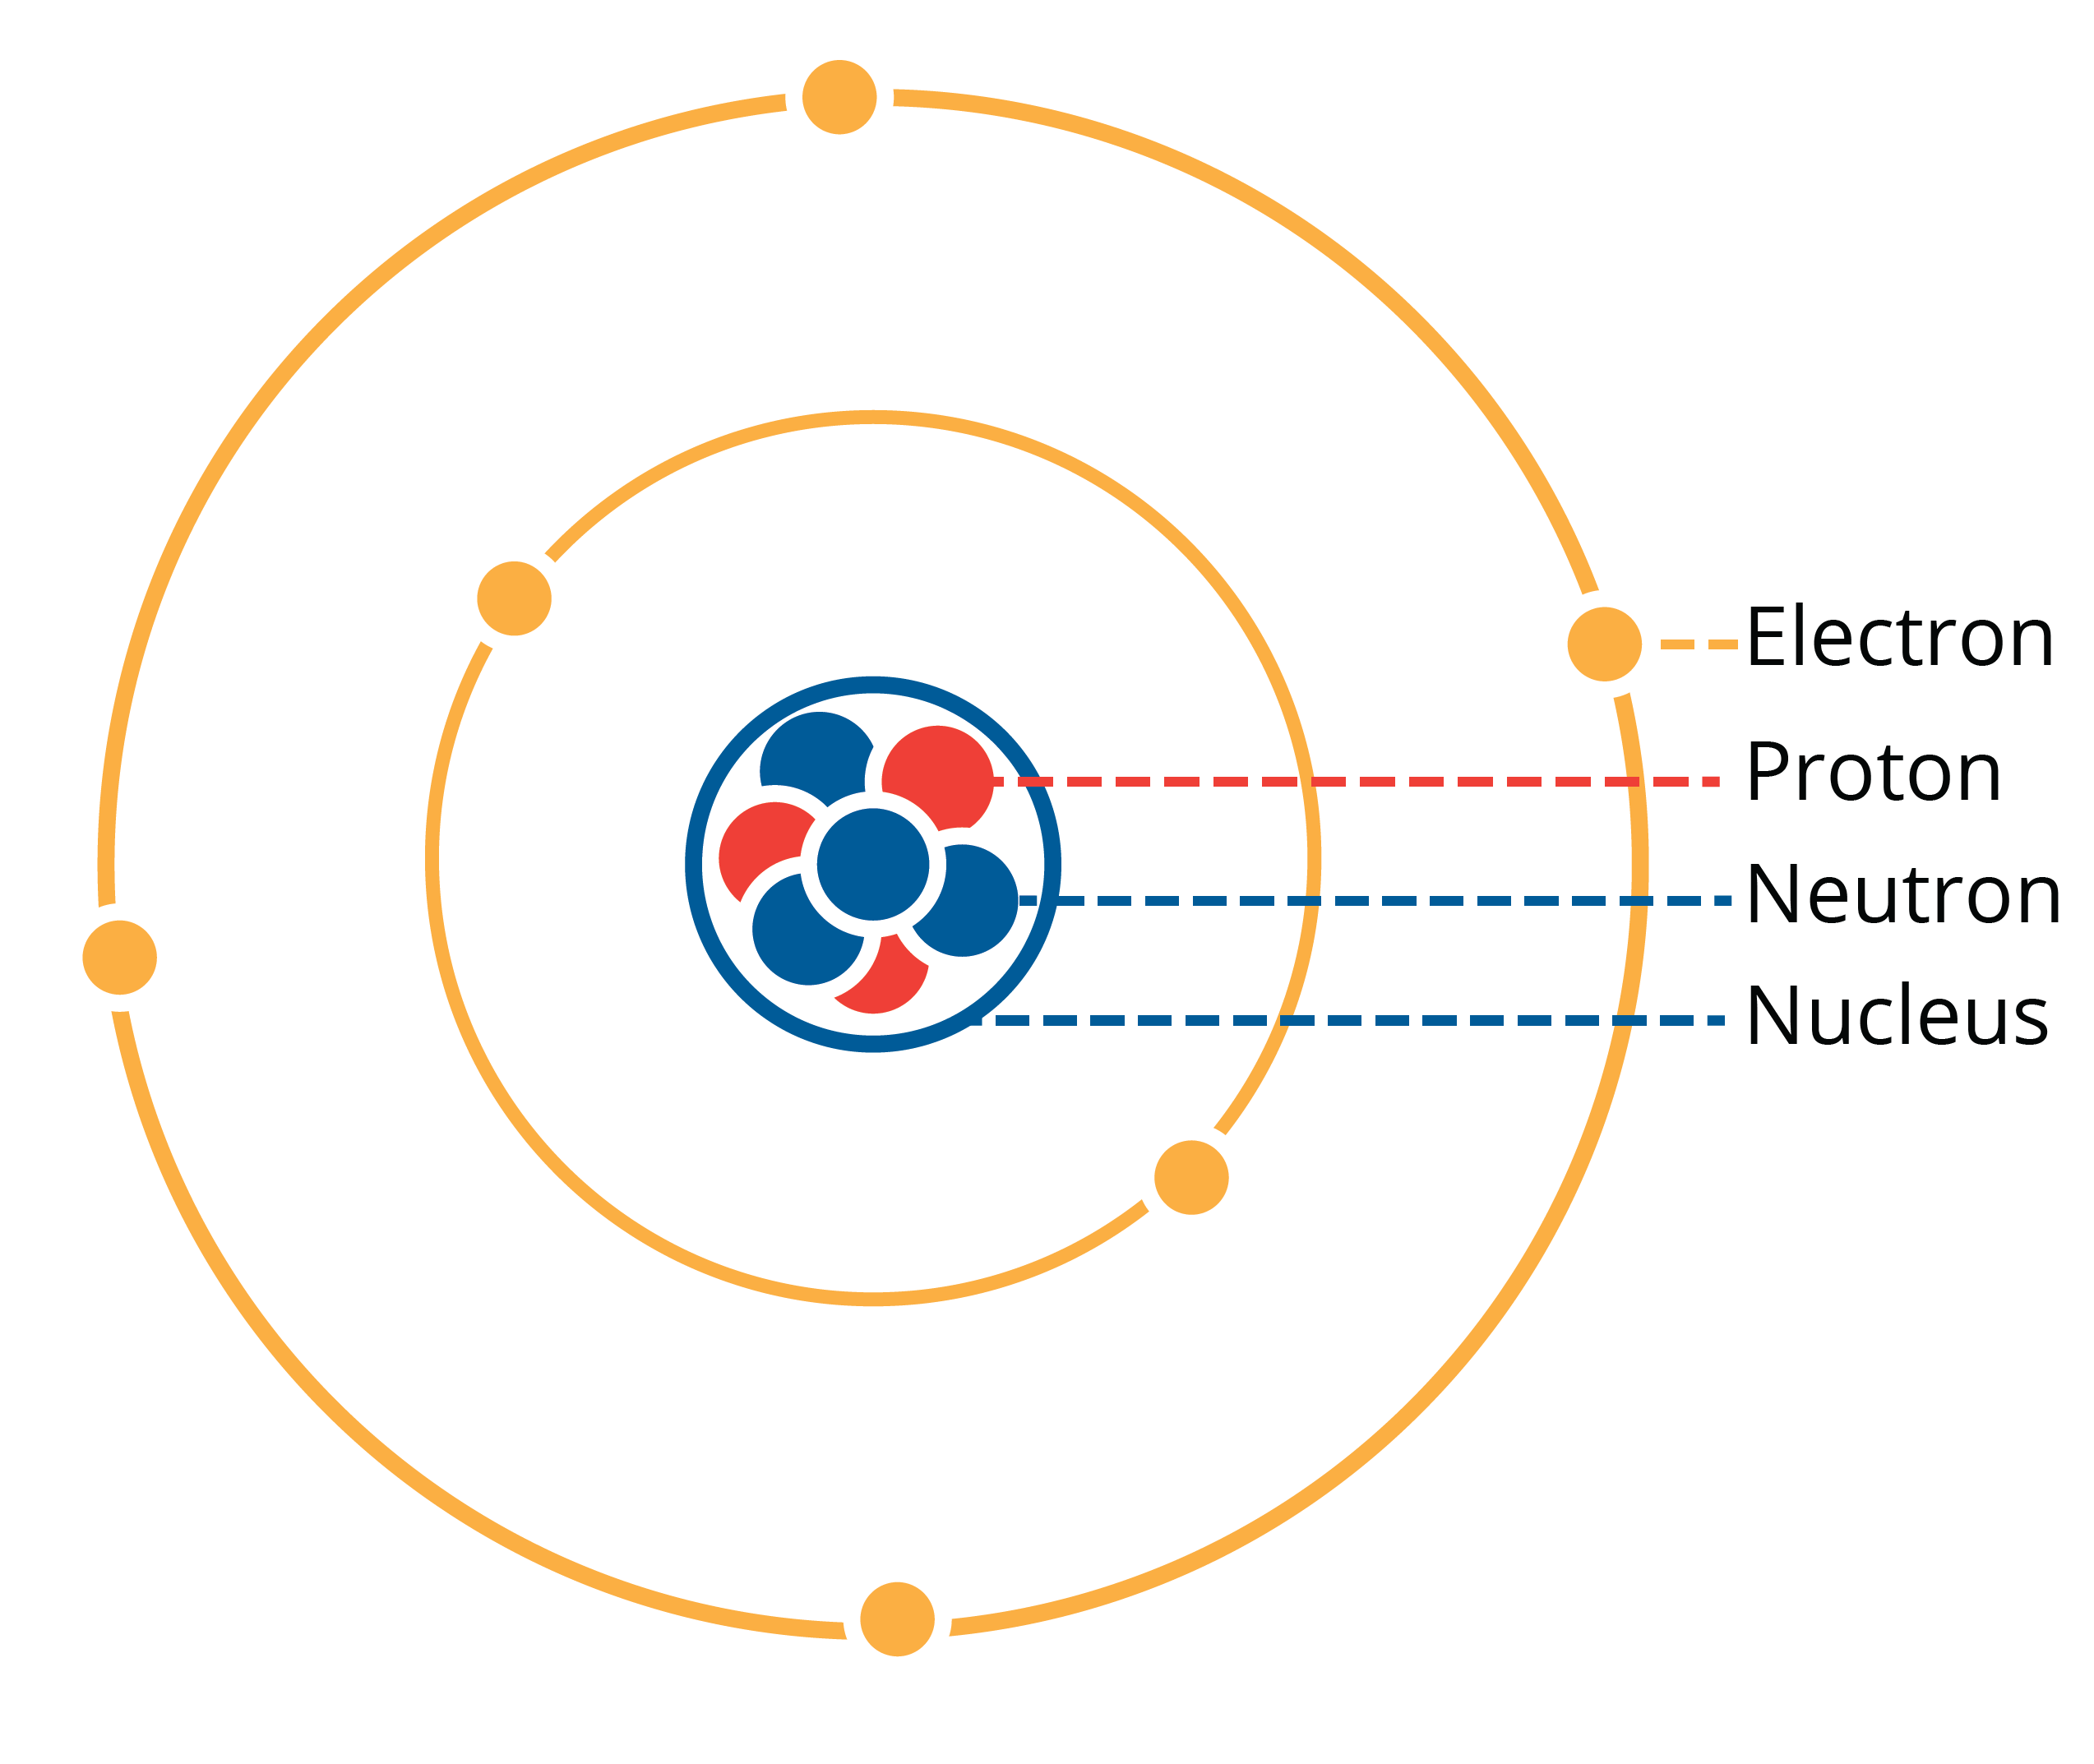
\includegraphics[width=2.5in]{atom1.png}
\caption{}
\label{fig:atom1}
\end{wrapfigure}

What is this ordinary matter made of? All things (including the air around you) 
are made of atoms. Atoms are incredibly tiny --- there are more atoms in a drop 
of water than there are drops of water in all the oceans.
% ADD: If you want a better visual of the scale: https://htwins.net/scale2/, start at around 10^-8

Every atom has a nucleus that contains protons and neutrons. Orbiting around the
nucleus is a cloud of electrons. However, the mass of the atom comes mainly from 
the protons and neutrons, since they are about 2000 times as massive as an 
electron! These three particles, protons, neutrons, and electrons, are called
\textit{subatomic particles}. (See figure \ref{fig:atom1}.) \index{protons} 
\index{neutrons} \index{electrons} \index{subatomic particle}

\section{Atoms and Their Models}
Over the history of science, there have been many ideas about the structure of
atoms. This history is a good example of how science develops: unexpected
results drive scientists to update their models, moving us closer and closer to
a true model of the atom.

During his investigations into the behavior of gases, John Dalton noted that 
different elements combine in strict ratios. For example, he noted that nitrogen 
and oxygen combine in a 1:1 and 1:2 fashion, but no ratio in between.

\begin{wrapfigure}{l}{3in}
\noindent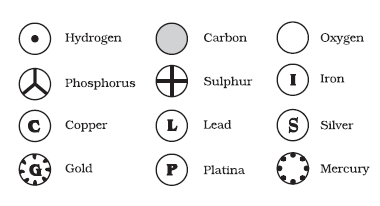
\includegraphics[width=2.5in, trim={0 0.5cm 0 0.5cm}, clip=true]{daltons_model.png}
\caption{Dalton modeled atoms as indivisible and unique.}
\end{wrapfigure}

This first model of the atom is rudimentary; each element is a unique atom,
and those atoms cannot be subdivided. The atom is modeled as one large, solid,
uniform, and neutral object. British physicist J.J. Thomson discovered that
atoms could be split into a light, negatively charged particle and a heavier,
positively charged particle (we now know this is the nucleus, the dense
grouping of protons and neutrons in the center of an atom).

Suddenly, the atom went from neutral and indivisible to made of different types
of charged particles. Further experiments by Ernest Rutherford showed the atom
to be mainly empty space, further updating scientists' model of the atom.
Subsequently, Bohr explained the phenomena of spectral lines (we will discuss
this further in Sequence 2) by modeling electrons as being restricted to
orbiting specific distances from the nucleus.

\begin{wrapfigure}{r}{3in}
\noindent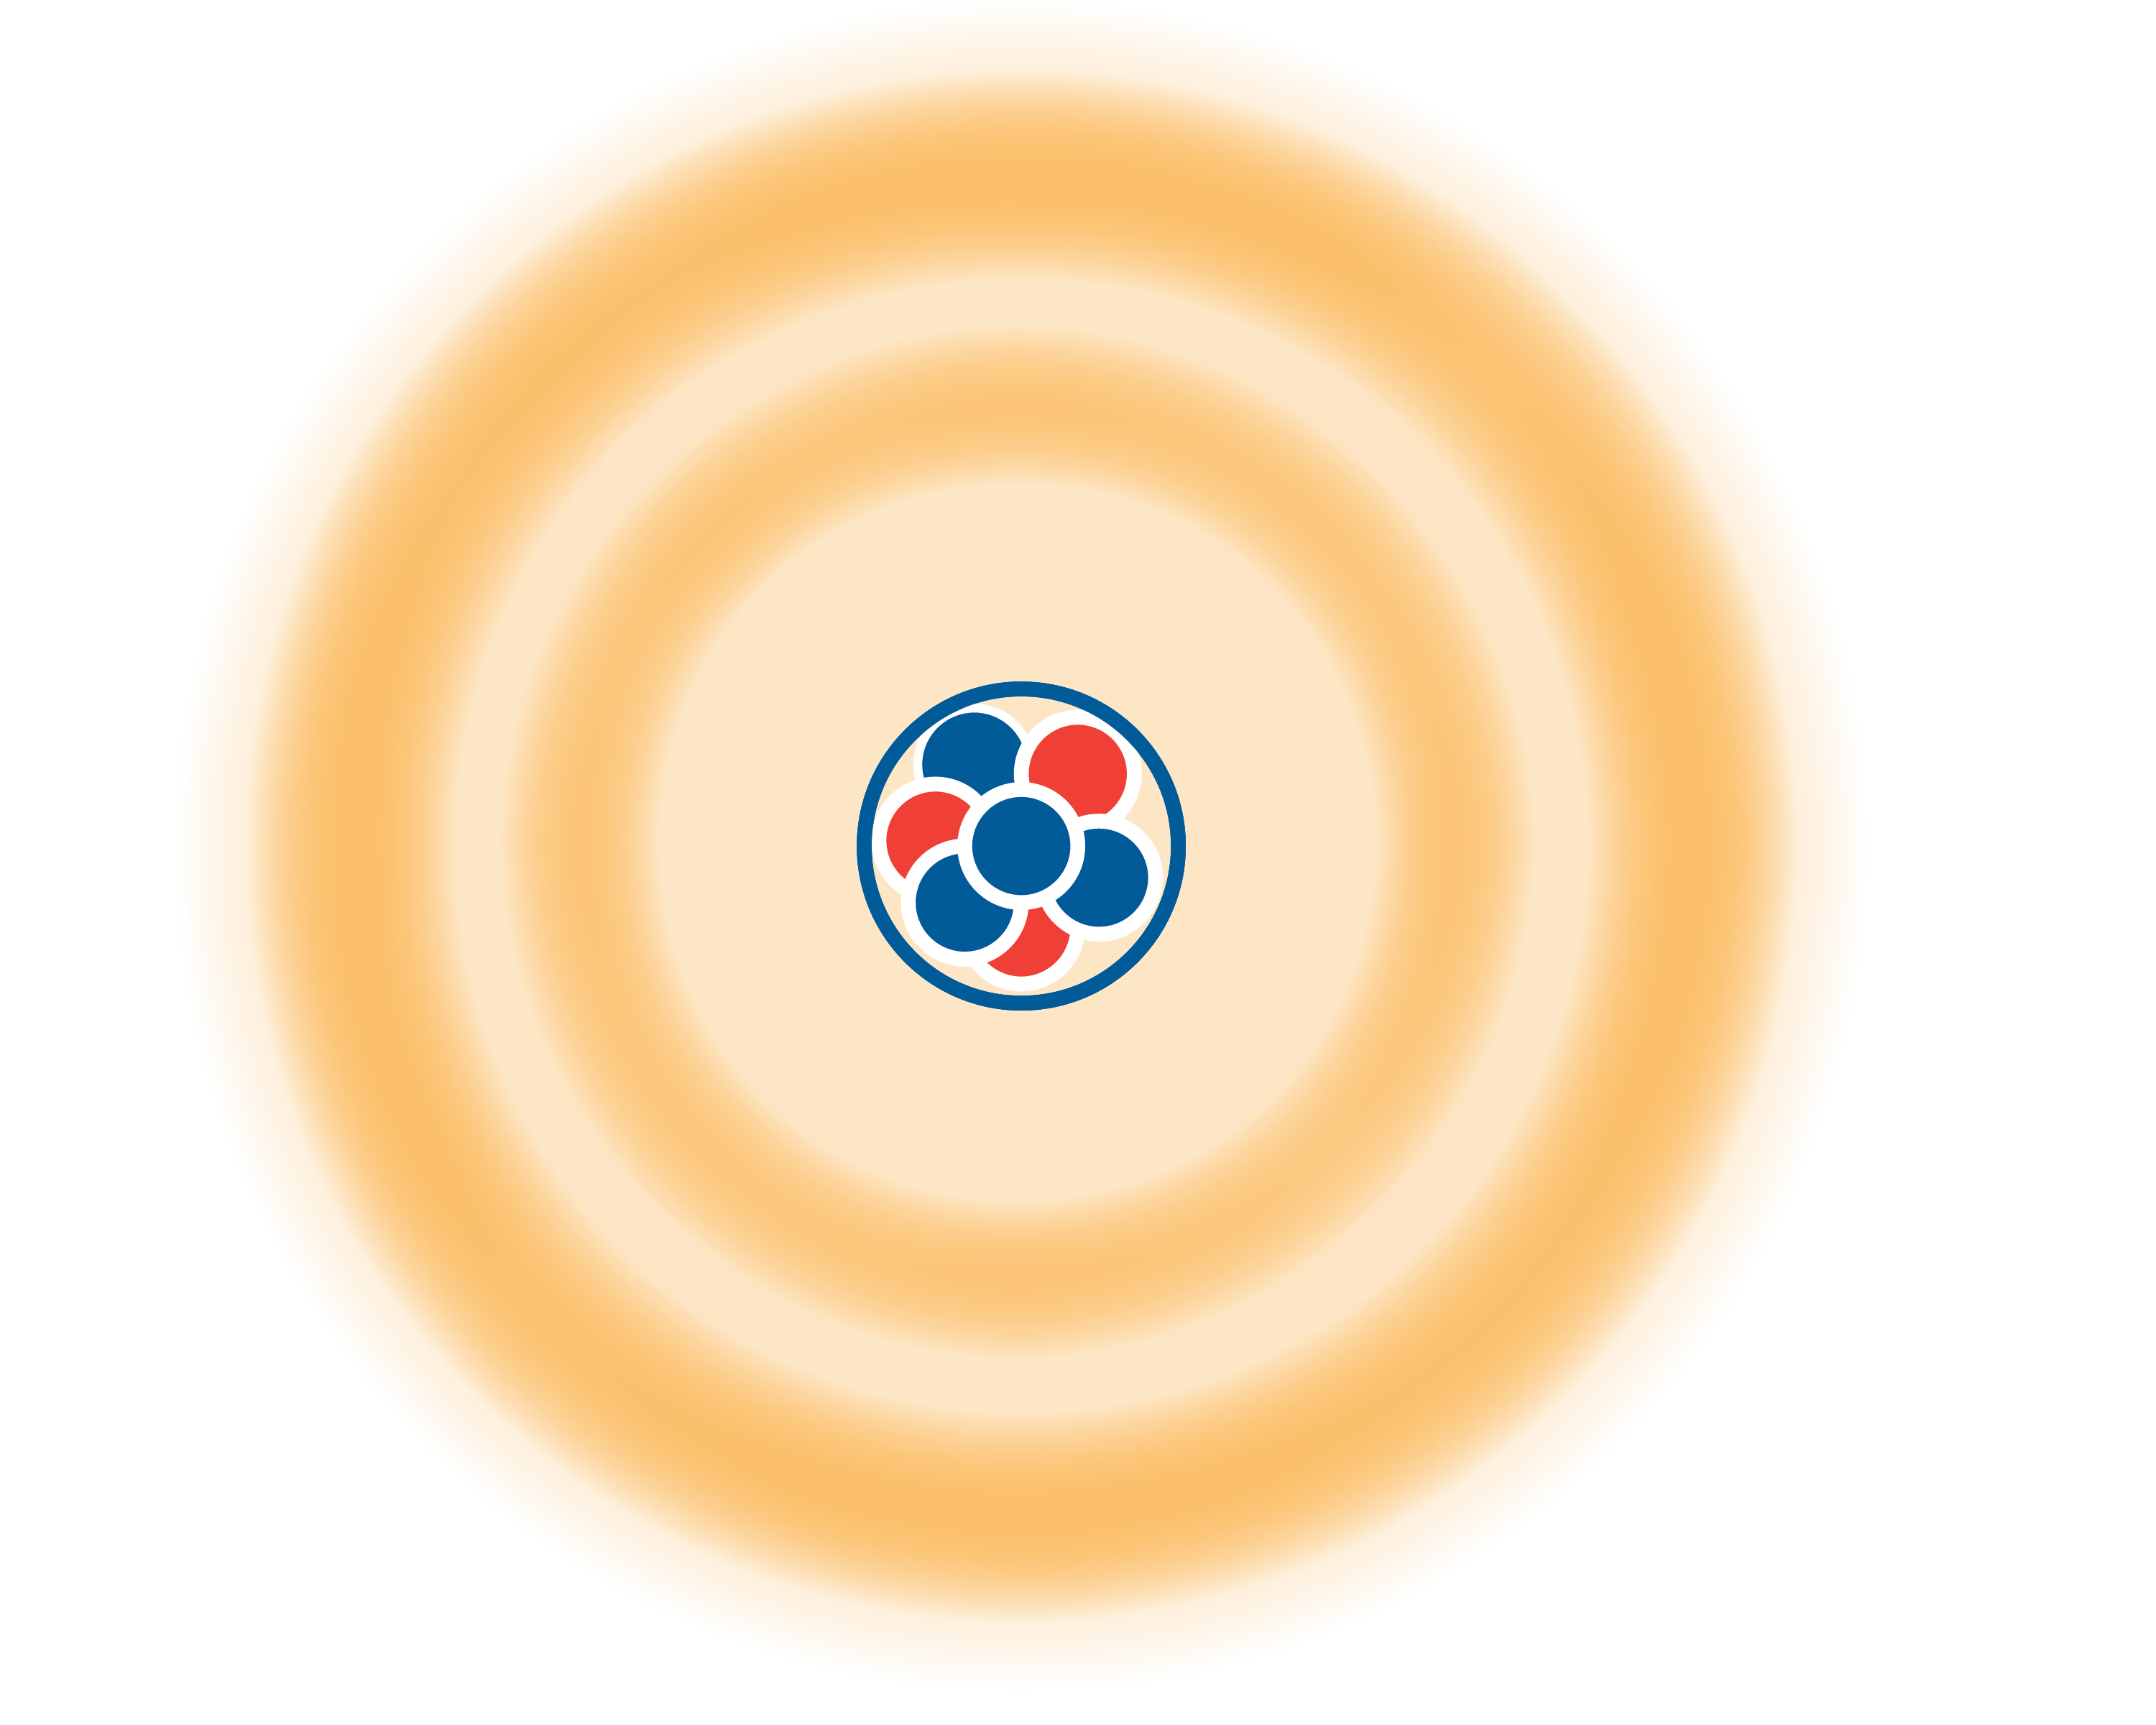
\includegraphics[width=3in]{atomCloud.png}
\caption{}
\label{fig:atomCloud}
\end{wrapfigure}

This is likely the model you are most familiar with seeing, and it is the one we
will use most often in this text. The first figure shown in this chapter is a Bohr
model: it shows the protons and neutrons in the nucleus, and models the electrons 
as moving in discrete orbits around the nucleus. 

However, the Bohr model is slightly inaccurate. While it is a convenient model for
thinking about atoms, in reality, electrons don't neatly orbit the nucleus.
Scientists don't know exactly where an electron will be in relation to the
nucleus, but they do know where it is most likely to be. They use a cloud that is
thicker in the center but fades out at the edges to represent an electron's
position (see figure \ref{fig:atomCloud}).

\begin{wrapfigure}{r}{3in}
\noindent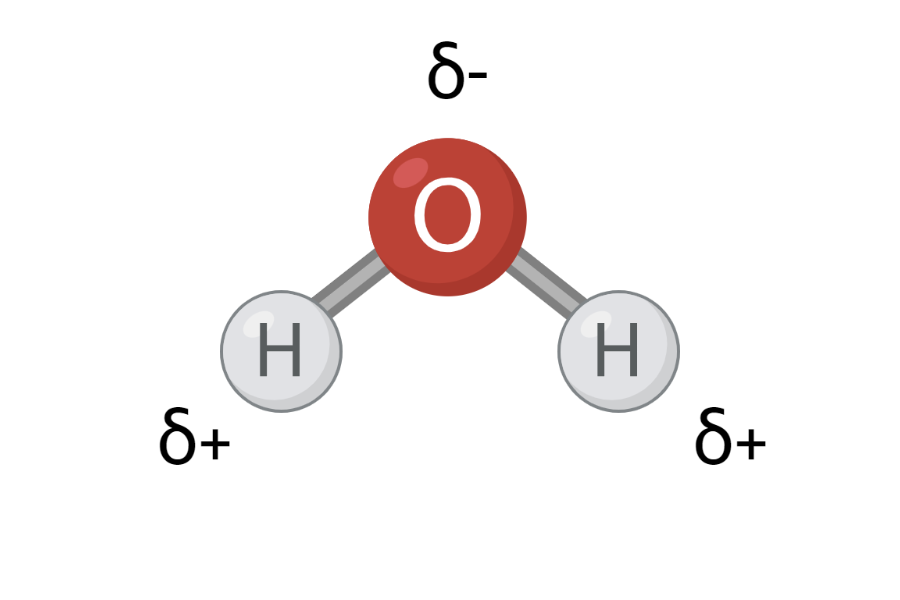
\includegraphics[width=3in]{water_polar.png}
\caption{}
\label{fig:water_polar}
\end{wrapfigure}

While the cloud model is more accurate, we will use the Bohr model as it
allows the viewer to easily and quickly assess the number and arrangement of
electrons.

\subsection{Classifying Atoms}

We classify atoms by the numbers of protons they have. An atom with one proton
is a hydrogen atom, an atom with two protons is a helium atom, and so forth
(refer to periodic table on pg..). We say that hydrogen and helium are \textit{
elements} because the classification of elements is based on the proton number.
And we give each element an atomic symbol. Hydrogen gets $H$, helium gets $He$,
oxygen gets $O$, carbon gets $C$\index{elements}, and so on.

\subsection{When Atoms Combine}
When atoms of different elements combine, they make \textit{compounds}. Compounds
are substances made up of more than one element. Compounds can be 
\textit{molecules} or \textit{crystal lattices}. In the next section you'll learn
\textit{why} these different structures form. 

There are many kinds of compounds. You know a few:
\begin{itemize}
\item Table salt is crystals made of $Na^{+}$ and $Cl^{-}$ ions: a sodium atom 
that as lost an electron and a chlorine atom that gained an electron
\item Baking soda, or sodium bicarbonate, is $NaHCO_3$.
\item $O_2$ is the oxygen molecules that you breathe out of the air (air, a
blend of gases, is mostly $N_2$.).
\item Common quartz is $SiO_2$: silicon dioxide
\end{itemize}

The subscripts indicate what ratio of the elements are present in the compound. 
Each number indicates the ratio for the preceding element. A drop of water, 
$H_2O$, has twice as many hydrogen atoms as oxygen atoms. 

\textbf{Example}: What is the ratio of elements present in Epsom salt?

\textbf{Solution}: Epsom salt, chemical name magnesium sulfate, has the chemical formula $MgSO_4$. Therefore, the ratio of Mg:S:O is 1:1:4. 

%fixme molecule vs formula unit, ordering of bonds versus formulas

\begin{Exercise}[title = {Numbers of Atoms in Molecules}, label = num_atom]
Give the elemental ratio for each compound. 
\begin{enumerate}
\item methane, $CH_4$
\item copper (II) sulfate, $CuSO_4$
\item glucose, $C_6H_{12}O_6$
\end{enumerate}
\end{Exercise}

\begin{Answer}[ref = num_atom]
\begin{enumerate}
\item C:H = 1:4
\item Cu:S:O = 1:1:4
\item C:H:O = 6:12:6 = 1:2:1
\end{enumerate}
\end{Answer}

\section{Types of Matter}
One way to classify matter is by the types of chemical bonds that hold a 
material's atoms together. The nature of these bonds, in turn, affects the 
properties of the material. For now, all you need to know is there are three types
of chemical bonds: metallic, covalent, and ionic. Materials held together with the
same type of bonds tend to have similar properties. For example, copper, bronze, 
iron, and steel (all containing metallic bonds) are all shiny, ductile, malleable,
and good conductors of heat and electricity. On the other hand, Epsom salt and 
table salt for large crystals, have very high melting points, and are poor 
conductors of electricity in their pure form. These two substances (Epsom and 
table salt) both contain ionic bonds. 

\subsection{Ionic Compounds}
Ionic bonds are the electrical attraction between opposite-charged ions. When a 
neutral atom gains or loses an electron it becomes an \textit{ion} (a charged 
atom), and oppositely-charged ions are attracted to each other. Which atom gets 
the electron and which loses it is based on their relative 
\textit{electronegativities}.\index{electronegativity} Electronegativity is simply
a measure of how strongly an atom can attract electrons to itself. In general, 
elements on the right side of the periodic table are more electronegative than 
elements on the left side. There are also polyatomic ions: groups of atoms held 
together with covalent bonds that have an overall charge (figure ... shows a Bohr 
model of a phosphate polyatomic ion, as an example). For now, we'll focus just on 
ionic bonds between monoatomic ions, like in table salt. You'll learn more about 
polyatomic ions and the compounds they form in Sequence 2. 

\begin{wrapfigure}{l}{3in}
\noindent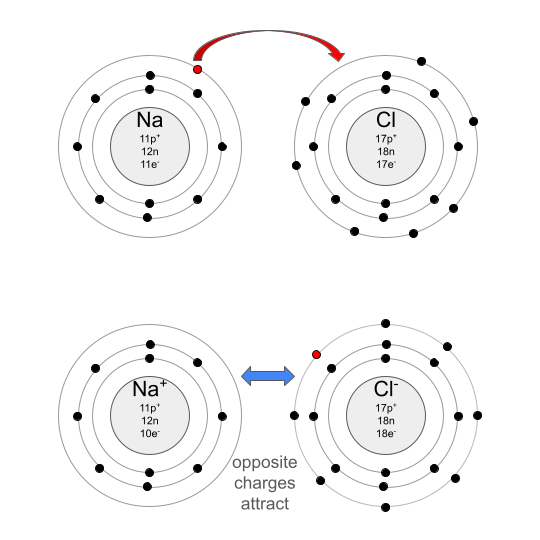
\includegraphics[width=3in]{NaCl_xfer.png}
\caption{}
\label{fig:NaCl_xfer}
\end{wrapfigure}

Let's examine how a simple ionic compound is formed: sodium chloride, also known 
as table salt, is made up of sodium and chlorine atoms (see figure 
\ref{fig:NaCl_xfer}). When sodium and chlorine come in contact with each other, 
electrons move from the sodium to the chlorine, making a sodium \textit{cation} 
(positively-charged ion) and a chloride \textit{anion} (negatively-charged ion). 
Yes --- chlor\textit{ide} is correct! When naming an anion, the ending of the 
element name changes to \textit{-ide}. Once the sodium cation and chloride anion 
are formed, their opposite charges attract them to each other, like north and 
south magnet poles. 

\begin{wrapfigure}{l}{3in}
\noindent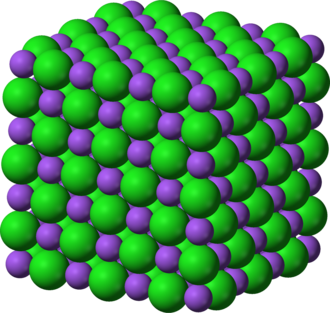
\includegraphics[width=2in]{NaCl_lattice.png}
\caption{}
\label{fig:NaCl_lattice}
\end{wrapfigure}

When there are many, many sodium and chloride ions around, they spontaneously 
arrange themselves in a pattern, giving ionic compounds their characteristic 
crystal structure (see figure \ref{fig:NaCl_lattice}). Because the electrons are 
tightly held be each ion, ionic substances don't conduct electricity well as 
solids. The atomic crystal lattice also determines the shape of the macroscopic 
crystals. Salt crystals are generally cubic, while other crystals (like quartz) 
form hexagonal prisms. You'll learn how to predict the atomic and macroscopic 
crystal structure of different compounds in Sequence 2. 

\subsection{Covalent Compounds}
Water is an example of a covalent compound: it is made of two hydrogen atoms 
covalently bonded one oxygen atom (see figure \ref{fig:water_polar}). The result 
is a water molecule\index{molecules}. The different atoms cluster together 
because they share electrons in their clouds. This is the nature of a 
\textit{covalent bond}\index{covalent bond}: it is formed when atoms share electrons.
Sometimes, electrons are shared evenly, but in water, they are shared unevenly. 
Due to the difference in electronegativity between hydrogen and oxygen, the 
shared electrons are more attracted to the oxygen atom than the hydrogen atoms, 
so they spend more time on the oxygen atom. As a result, the oxygen side of a 
water molecule has a slight negative charge, while the hydrogen atoms have a 
slight positive charge. The slight charges are represented with a lower case 
Greek letter delta, $\delta$. When electrons are shared unevenly, we call this a
\textit{polar} covalent bond, because there are positive and negative poles at 
either end of the bond. \index{polar bond} \index{non-polar bond}

When covalent bonds form between two elements of similar electronegativities, 
the electrons are shared evenly. We call this a \textit{non-polar} covalent bond. 
Oil is an example of a non-polar covalent substance. Different oils have different
combinations, but all oils are made mainly of carbon and hydrogen, which have similar
electronegativities. For both polar and non-polar covalent bonds, the electrons 
are still held tightly, even if they are shared. Those electrons don't move to 
another molecule: they move around within the molecule they are already a part 
of. Since electrons don't flow freely in covalent substances, they are also poor 
conductors of electricity. But, they generally have lower melting and boiling 
points than ionic compounds. 

What happens when you try to mix oil and water? They don't mix well! This is due 
to the difference between their bond types. Polar substances, like water, mix best
with other polar substances, while non-polar substances, like oils, mix best with 
non-polar substances. You'll learn more about why this is in Sequence 2.

\subsection{Metallic Compounds}
You may already know that metals (both pure and alloyed) are excellent conductors of electricity and heat. This is a consequence of their metallic bonds. 
%fixme complete section, pure vs alloys, free flowing electrons



\section{Energy and Work}

Energy is defined as the ability to do work, but what does this mean? First, we 
need to understand what \textit{work} is. When you lift an object into the air, 
you are doing work on that object. When water turns a turbine in a hydroelectric 
plant, the water is doing work on the turbine. And when you hit the brakes on your
car, the brake pads are doing work on the tires (albeit, negative work). 
\textit{Energy} is being transferred between these pairs of objects when work is 
done. 

Some everyday examples of energy include:
\begin{enumerate}
\item The Calories in your food
\item The light from the Sun
\item Heat in the Earth's mantle
\item The motion of a spinning wheel
\end{enumerate}

Some types of energy are easy to visualize, while others are not. Energy is what 
moves from one object to another when work is being done. When you lift 
something, the energy stored in your body (in the form of sugar and fat) is 
transferred to the object, accelerating it upwards. Your body continues to 
transfer energy as you lift the object against gravity. When you've lifted it as 
high as you can, most of the energy your body lost (we call this "burning 
Calories" colloquially) is stored as \textit{potential energy}, due to the 
object's height. 

Another example is a simple circuit connecting a battery and a light bulb. The 
battery has stored potential energy. When the circuit is complete, the potential 
energy in the battery is transferred to electrons in the light bulb, causing them 
to move and gain kinetic energy. In the light bulb's filament (we are referencing 
old, non-LED light bulbs here!), the electrons encounter resistance, which slows 
them down. The energy the electrons lose in this process is being transformed into 
light and heat, lighting your room. 

%fixme edit/rehome material below



\section{Chemical Reactions}

\begin{wrapfigure}{l}{3in}
\noindent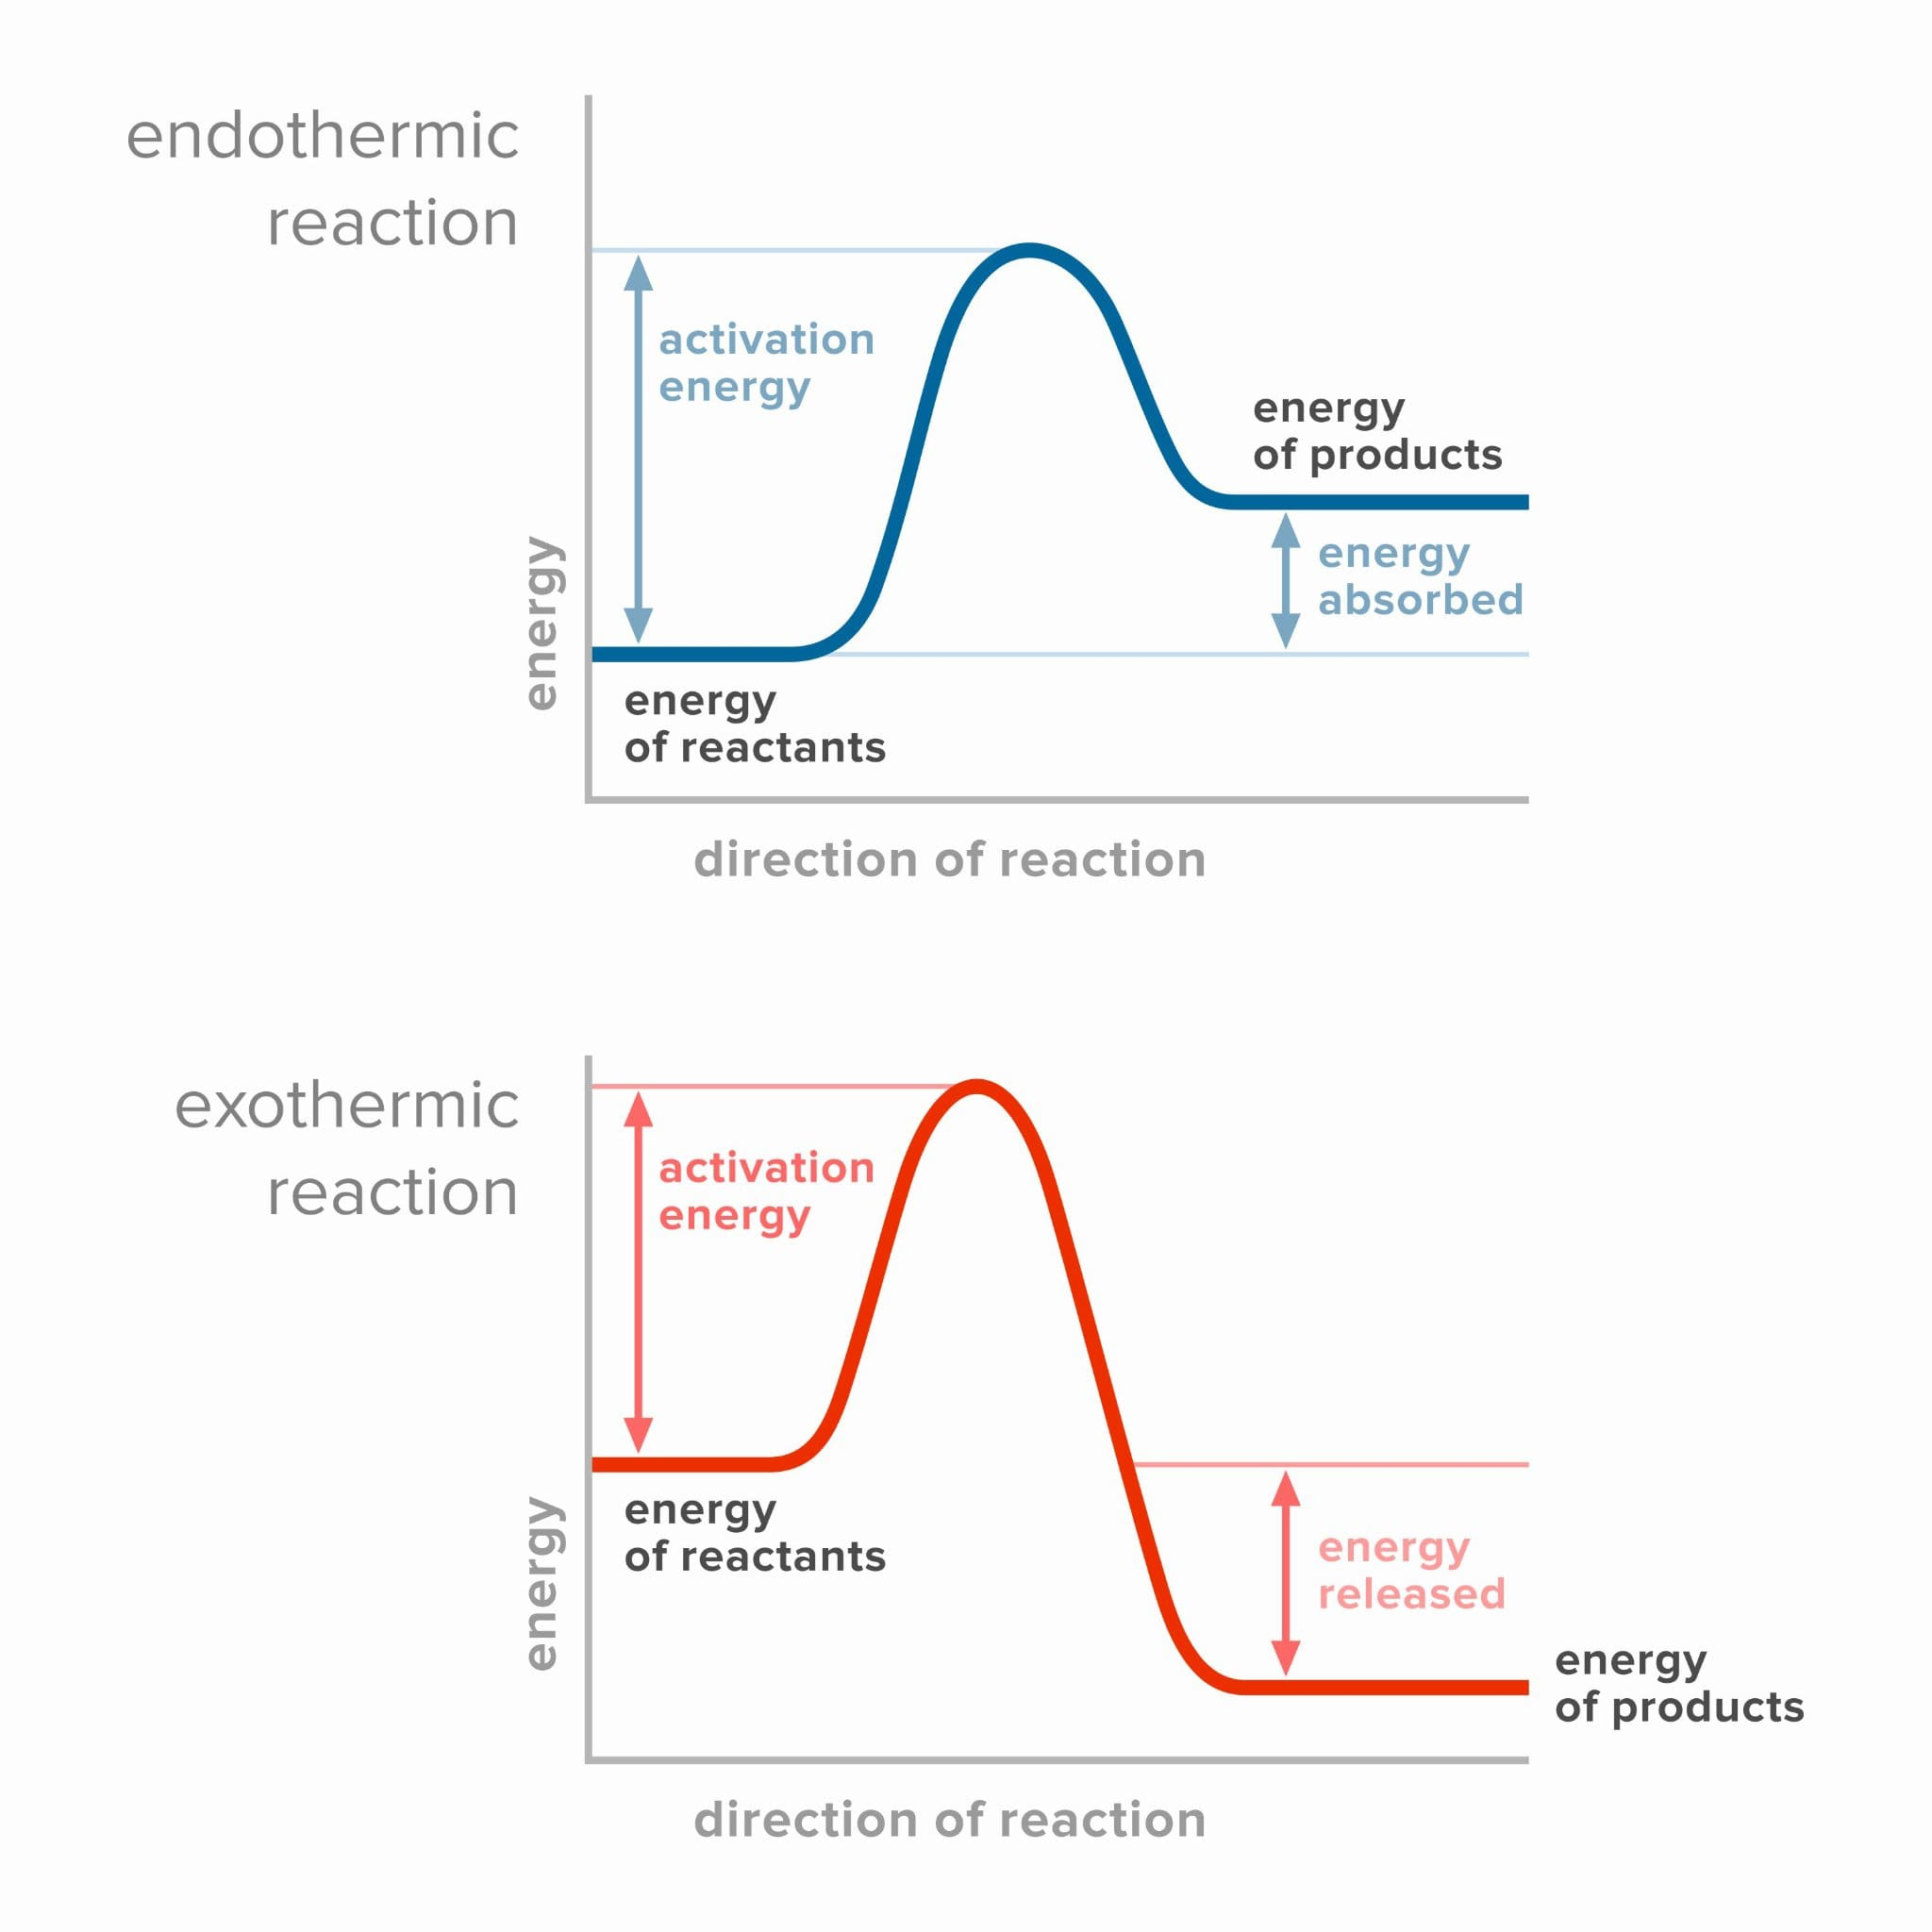
\includegraphics[width=3in]{exo_endo_diagrams.png}
\caption{}
\label{fig:exo_endo_diagrams}
\end{wrapfigure}

Sometimes two hydrogen atoms form a molecule ($H_2$). Sometimes two oxygen
atoms form a molecule ($O_2$). If you mix these together and light a match,
they will rearrange themselves into water molecules. This is called a \textit{
chemical reaction}. In any chemical reaction, the atoms are rearranged into new
molecules.\index{chemical reaction}

Some chemical reactions (like the burning of hydrogen gas described above) are
\textit{exothermic} --- that is, they give off energy. Burning hydrogen gas
happens quickly and gives off a lot of energy. If you have enough, it will make
quite an explosion! \index{exothermic}

Other chemical reactions are \textit{endothermic} --- they consume energy.
Photosynthesis, the process by which plants consume energy from the sun to make
sugar from $CO_2$ and $H_2O$ requires an endothermic chemical reaction.\index{endothermic}

Examine the diagrams in figure \ref{fig:exo_endo_diagrams}. The $x$-axis 
represents time - time passes as wemove from left to right across the diagram. 
At the far left, the energy of the reactants (the ingredients that go into the 
reaction) is shown. At the far right, the energy of the products (what is made in 
the chemical reaction) is shown. The red diagrams shows an exothermic reaction: 
the products (what is made) have less energy than the reactants (the "ingredients"
that start the reaction). Since energy is never created or destroyed, where did 
the energy go? It is released as heat. So, exothermic reactions release heat.

Now, look at the endothermic reaction diagram (the blue one). Based on the
relative energies of the reactants and products, do you expect and endothermic
reaction to release or absorb heat? Absorb! Since the products have more
energy, they must have absorbed energy, in the form of heat, from the surroundings.

What does this look and feel like in real life? If an exothermic reaction were
happening in a glass beaker, you would feel warmth if you held the beaker. The
heat is leaving the beaker and entering your hand, which feels warm. What
about an endothermic reaction? Many students think that since an endothermic
reaction absorbs heat, it must be getting hot. This is incorrect:
\textit{exothermic} reactions feel hot. If an endothermic reaction were
happening in a beaker and you touched the beaker, it would feel \textbf{cold}.
Why? Well, if the reaction is absorbing heat, then heat must be leaving it
surroundings (your hand) and entering the reaction (this heat energy is turned
into chemical energy that is stored in the new chemical bonds that are
forming). So your hand feels cold. %fixme: models showing flow of heat in/out of system for chemical reactions.

\section{Mass and Acceleration}

Each atom has a mass, which means everything made up of those atoms has mass as 
well (and that's pretty much everything!). We measure mass in grams. A paper clip 
is about 1 gram of steel. An adult human can have a mass of 70,000 grams, so for 
larger things, we often talk about kilograms, which is 1000 grams.

The first interesting thing about mass is that objects with more mass
require more force to accelerate. For example, pushing a bicycle so
that it accelerates from a standstill to jogging speed in 2 seconds
requires much less force than pushing a train so that it accelerates
at the same rate.


\begin{mdframed}[style=important, frametitle={Newton's Second Law of Motion}]

The force necessary to accelerate an object of mass $m$ at an acceleration of
$a$ is given by:
$$F = m a$$

This means the force is equal to the mass times the acceleration.

\end{mdframed}

What are the units here? We already know that mass is measured in
kilograms. We can measure velocity in meters per second, but that is
different from acceleration. Acceleration is the rate of change in
velocity. So if we want to go from 0 to 5 meters per second (that's
jogging speed) in two seconds, that is a change in velocity of 2.5
meters per second every second. We would say this acceleration is $2.5
m/s^2$.

\subsection{Calculating Acceleration}
As suggested above, acceleration is a change in velocity. It is calculated by
dividing the change in velocity by the time it takes to make that change.

\begin{mdframed}[style = important, frametitle = {Calculating Acceleration}]
The acceleration of an object from an initial velocity, $v_i$, to a final
velocity, $v_f$, over a period of time, $t$, is given by:

$$a = \frac{v_f - v_i}{t}$$
\end{mdframed}

\textbf{Example}: Your car can go from zero to 60 mph in 3 seconds. What is the
acceleration in $m / s^2$?

\textbf{Solution}: First, let's convert from the imperial units of miles per
hour to the SI units of meters per second. You can do this using a search engine, 
but we will show how to do it by hand below. (You will learn more about this 
method in the Units chapter).

$$\frac{60 \text{ miles}}{1 \text{ hour}} \cdot \frac{1.61 \text{ km}}{1 
\text{ mile}} \cdot \frac{1000\text{ m}}{1\text{ km}} \cdot \frac{1\text{ hour}}{
3600\text{ seconds}} \approx \frac{26.82\text{ m}}{s}$$

Now we have the starting velocity (0 m/s), the ending velocity (26.82 m/s), and 
the time (3 s), and we can find the acceleration:
$$a = \frac{v_f - v_i}{t} = \frac{26.82\frac{m}{s} - 0\frac{m}{s}}{3s} \approx 
8.94 \frac{m}{s^2}$$

\subsection{Determining Force}
What about measuring force? Newton decided to name the unit after himself: The
force necessary to accelerate one kilogram at $1 m/s^2$ is known as \textit{a
newton}. It is often denoted by the symbol $N$.

$$1 N = 1 \frac{kg \cdot m}{s^2}$$

\textbf{Example}: If the car in the above example has a mass of 1500 kg, how much 
force does the engine use to accelerate the car?

\textbf{Solution}: We have already found the car's acceleration: 8.94 $m/s^2$. 
With the mass and acceleration, we can use Newton's Second Law to find the force 
needed to accelerate the car:
$$F = m \cdot a = 1500\text{ kg} \cdot 8.94 \frac{m}{s^2} = 13410\text{ N}$$

\begin{Exercise}[title={Acceleration}, label=acceleration_train]

While driving a bulldozer, you come across a train car (with no brakes
and no locomotive) sitting on a track in the middle of a city. The train car
has a label telling you that it has a mass of 2,400 kg. There is a time-bomb
welded to the interior of the train car, and the timer tells you that
you can safely push the train car for 120 seconds. To get the train
car to where it can explode safely, you need to accelerate it to 20 meters per
second. Fortunately, the track is level and the train car's wheels have
almost no rolling resistance.

With what force, in newtons, do you need to push the train for those 120 seconds?

\end{Exercise}
\begin{Answer}[ref=acceleration_train]
If you accelerate to 20 m/s in 120 s, the acceleration is:
$$a = \frac{v_f - v_i}{t} = \frac{20\text{ m/s} - 0\text{ m/s}}{120\text{ s}} = 
\frac{1}{6} \frac{m}{s^2}$$

To achieve this acceleration, you will need to apply a force of:
$$F = m \cdot a = 2400\text{ kg} \cdot \frac{1}{6} \frac{m}{s^2} = 400\text{ }N$$
\end{Answer}



%FIXME Global layout note: Let's discuss adding Title's and Captions to all graphics.\\

%For example:\\
%TITLE: Mass versus Weight\\
%CAPTION: Human Earth weight: 150lbs / Moon weight:??lbs\\
%Potato Earth weight: .25lbs / Moon weight: ??lbs \\

%FIXME:
%Allison thinks it would be funny if the person in the graphic were holding a potato and we also added the weight and mass of the potato to the caption. No worries if this type of edit isn't in the budget!

%FIXME: What are your thoughts about using the metric system consistently -- in which case we'll replace pounds here with kilos. Max notes: we should explicitly use kilos for mass and pounds or newtons for weight. Kilos are a scalar measure of the amount of matter and pounds are a vector force of gravity on a particular piece of matter. Many students struggle to differentiate between mass and weight at a theoretical level due to casual comparison between pounds and kilos.

\graphicspath{{../../Chapters/atomic_mass/en_US}}
\chapter{Atomic and Molecular Mass}

%fixme add hook

\section{Reading a Periodic Tile}

Let's look at the different information shown on a periodic tile:

\begin{center}
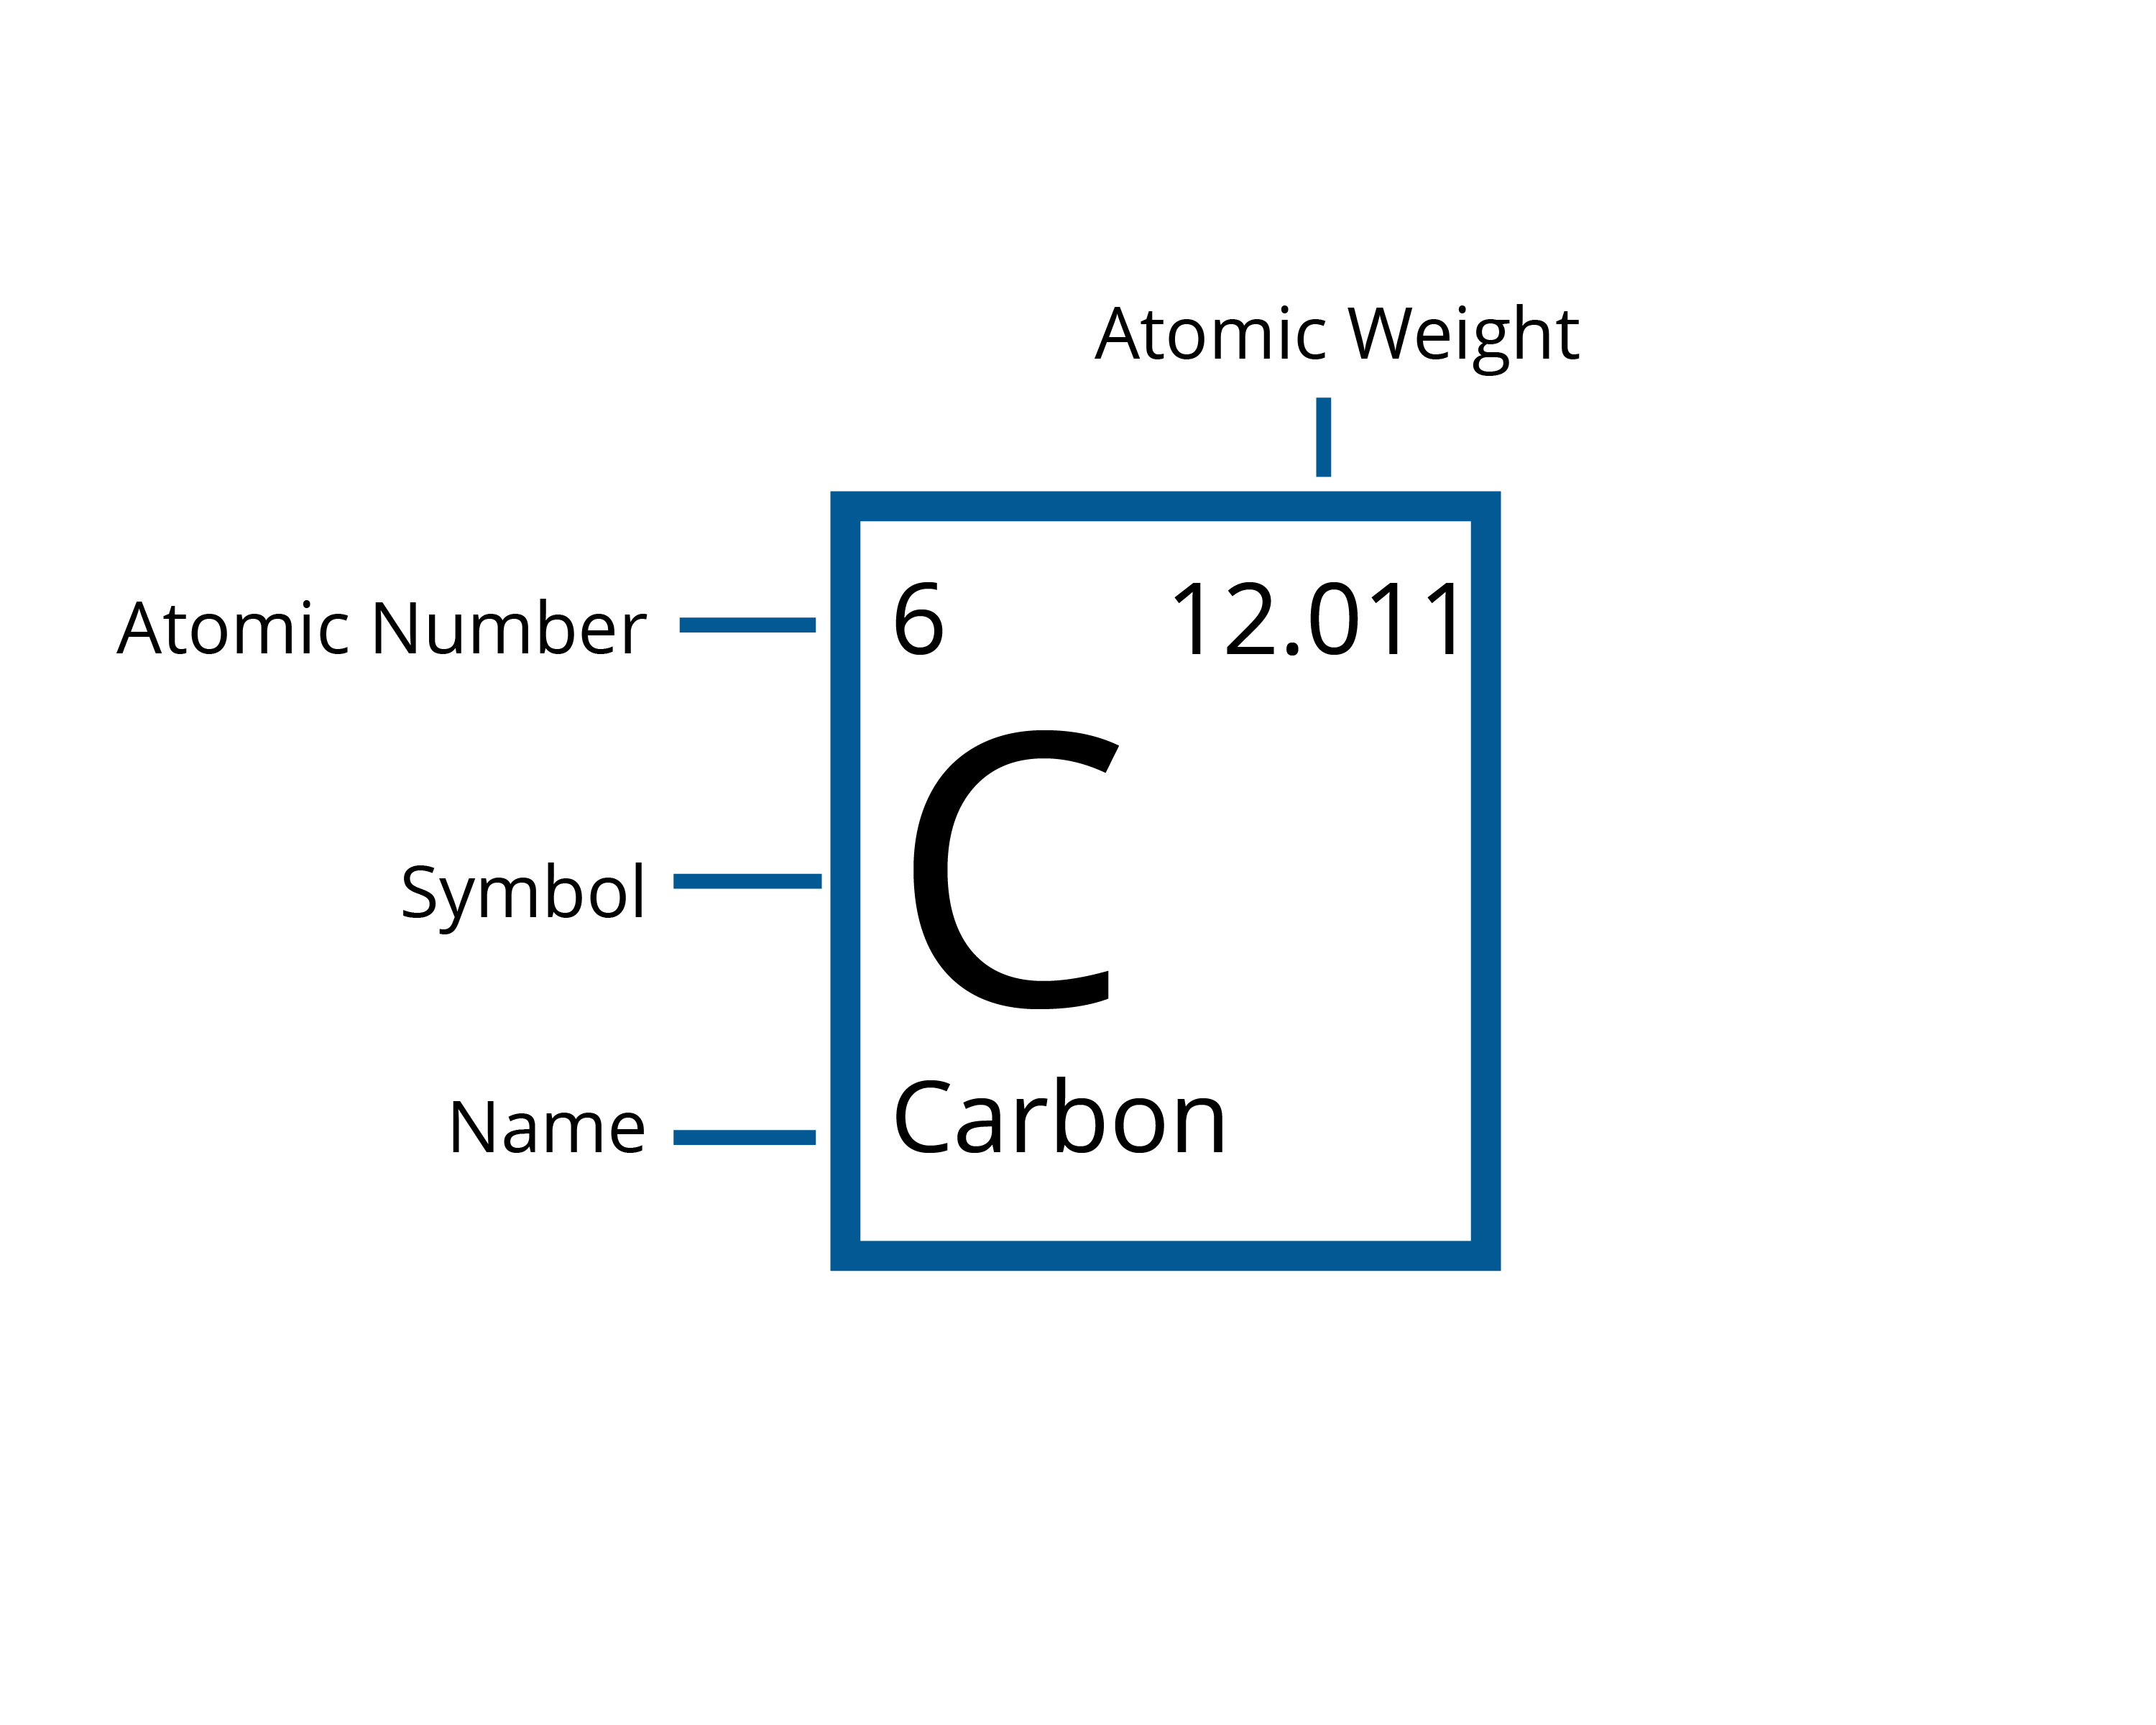
\includegraphics[width = 4in]{element.png}
%fixme change "weight" to "mass" or remake image
\end{center}

The four things we learn from a periodic tile are:
\begin{enumerate}
\item the symbol: as discussed in the previous chapter, each element has a 
unique symbol. Element symbols are used when showing the structure of a molecule
and modeling chemical reactions. 
\item the atomic number: this is also unique for each element. Take a look at the
periodic table a few pages forward. Every tile has a unique atomic number, and 
the tiles are laid out in a generally increasing atomic number (you'll learn why
the periodic table is arranged this way in Sequence 2). 
\item the atomic weight: this is the average mass of all the atoms of that element
in existence. Just like your overall grade in a class is the weighted average of
all the individual grades you earned, atomic weight is the weighted average of the
masses of all the individual atoms of that element. This is also sometimes referred to as atomic mass.
\item the name: not all periodic tables show the name of an element on its tile.
This is why it is useful to know the symbols of common elements. 
\end{enumerate}

Recall from the previous chapter that we classify atoms by the number of protons
they have. What this means is that if we want to know what element an atom is, we
have to look at the number of protons. Take a look at the three carbon atoms below
and note what is the same and what is different among them:

\begin{center}
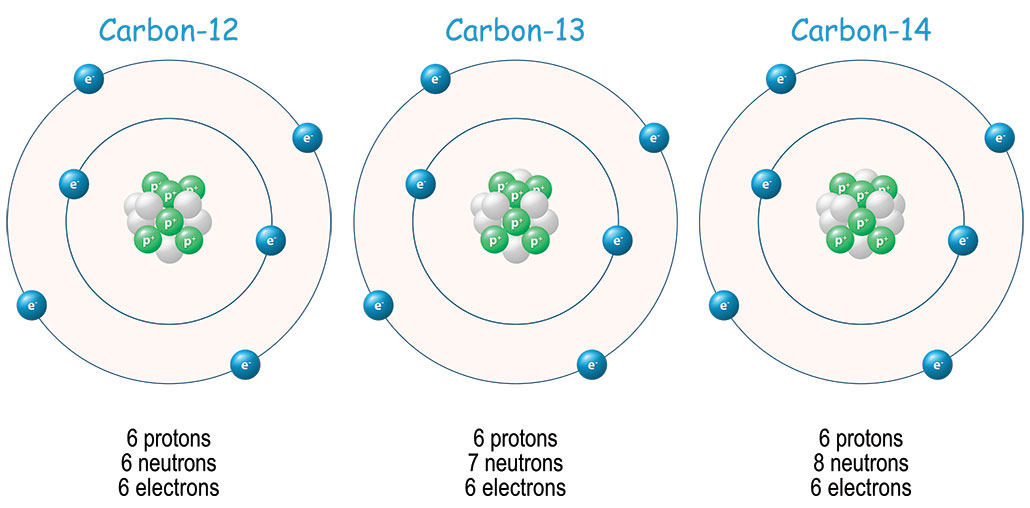
\includegraphics[scale=0.35]{carbon_iso.png}
\end{center}

These different versions of carbon all have 6 protons, which is also carbon's 
atomic number. This isn't a coincidence: the atomic number \textit{is} the number
of protons in every atom of an element. If I tell you an atom has 4 protons, you 
would find atomic number 4 and see that the element is beryllium. To know how many
protons an oxygen atom has, you would find its tile and see that it has atomic 
number 8. 

Ok, so now we know atoms of the same element have the same number of protons, and
that number is given by the element's atomic number. The difference between these
carbon atoms explains the other number on a periodic tile: the atomic mass. 

A proton and a neutron have about the same mass. An electron, on the other hand,
has much less mass: One neutron weighs about the same amount as 2000 electrons. 
This means that the mass of any object comes mostly from the protons and neutrons
in the nucleus of its atoms. \index{proton} \index{neutron}

We know how many protons an atom has by what element it is, but how do we know the 
number of neutrons?

\section{Mass of Atoms and Molecules}
As you've seen, a periodic tile for an element tells us the average mass of an 
atom of that element in Daltons or amus (atomic mass units). The average mass of a
carbon atom is 12.011 amu, and the average mass of an iron atom is 55.845 amu. 
Using the periodic table, determining the average mass of an atom is 
straightforward. What about molecules?

Consider water: $H_2 O$. It is made of 2 hydrogen atoms, each with an average 
mass of 1.008 amu, and one oxygen atom, with an average mass of 15.999 amu. To 
find the mass of the molecule, called \textit{molecular mass}, you simply add the 
masses of each of the atoms in the molecule. So, the molecular mass of water is 
1.008 amu + 1.008 amu + 15.999 amu = 18.015 amu. 

\begin{Exercise}[title = {Determining Molecular Mass}, label = molecular]
Find the molecular mass, in amu, of the following substances:
\begin{enumerate}
\item $CH_4$
\item $CuSO_4$
\item $C_6H_{12}O_6$
\end{enumerate}
\end{Exercise} 

\begin{Answer}[ref = molecular]
\begin{enumerate}
\item 12.011 amu + 4(1.008 amu) = 16.043 amu
\item 63.546 amu + 32.06 amu + 4(15.999 amu) = 159.602 amu
\item 6(12.011 amu) + 12(1.008 amu) + 6(15.999) amu = 180.156 amu
\end{enumerate}
\end{Answer}

\section{Mole Concept}

An atomic mass unit is a very, very, very small unit; we would much rather work in
grams. Grams are a large enough unit that you can develop a natural sense for how 
much a gram is. Additionally, while you can't see a single carbon atom with your 
eyes, you can see 10 grams of carbon (about enough to fill a pen cap). To convert
between the very, very, very small unit of amus to the tangible unit of grams, we 
use \textit{Avogadro's Number} (sometimes called \textit{Avogadro's Constant}).
\index{Avogadro's number}

Since 1 amu is defined as $1/12^{th}$ of the mass of a carbon-12 atom, carbon-12 
by definition has a mass of 12 amu. Additionally, Avogadro's number is the number 
of carbon atoms in 12.000 grams of pure carbon-12. This amount is called \textit{a
mole}. If you have 12 doughnuts, that's a dozen doughnuts. If you have 20 donuts, 
you have a score of donuts. 500 donuts: a ream of donuts. If you have $6.02214076 
\times 10^{23}$ doughnuts, you have a \textit{mole} of doughnuts. This isn't 
really a practical measurement, as a mole of doughnuts would be about the size of 
the earth. We use moles for small things like molecules.\index{mole} However, a mole is a not an abbreviation for a molecule. For a better 
idea about how large of a number Avogadro's number is, you can watch this video: 
\url{https://www.youtube.com/watch?v=TEl4jeETVmg}. 
A mole of carbon-12 has a mass of 12.000 g, but a mole of natural carbon (which
includes all the isotopes of carbon) has a mass of 12.011 g. The mole is defined 
such that one mole of an element is the same mass in grams as one atom is in amus.
Let's say you want to know how much a mole of $NaCl$ weighs. From the periodic 
table, you see that $Na$ has an atomic mass of 22.990 atomic mass units, and $Cl$ 
has 35.453 atomic mass units. One atom of $NaCl$ has a mass of $22.990 + 35.453 = 
58.443$ atomic mass units. This means a mole of $NaCl$ has a mass of $58.443$ 
grams. Handy, right? This is called the \textit{molar mass}. It is the mass of one
mole of a substance, and is given in units of $g/mol$ (grams per mole). The molar 
mass of NaCl is 58.443 g/mol. The molar mass of carbon is 12.011 g/mol. Using 
dimensional analysis and the molar mass, you can determine the mass of a given 
number of moles of a substance. 
% ADD: clarify here that g/mol is numerically equivalent to amus but conceptually different

\textbf{Example}: What is the mass of 2 moles of copper?

\textbf{Solution}: The conversion we will use is 1 mol Cu = 63.546 g Cu.
$$\frac{2 \text{ mol Cu}}{} \times \frac{63.546\text{ g Cu}}{1\text{ mol Cu}} = 
127.092\text{ g Cu}$$

Therefore, 2 moles of copper has a mass of 127.092 grams. 

You can also find the molar mass of a molecule, like methane. Just like with 
elements, a mole of a molecule has the same mass in grams as a single molecule has
in amus. 

\textbf{Example}: What is the mass of 3.5 moles of methane?

\textbf{Solution}: Methane ($CH_4$) has a molecular mass of 16.043 amu, which 
means 1 mole of methane has a mass of 16.043 grams. 

$$\frac{3.5\text{ mol }CH_4}{} \times \frac{16.043{ g }CH_4}{1\text{ mol }CH_4} = 
56.151\text{ g }CH_4$$

You can also use the molar mass to determine how many moles of a substance there 
are in a given mass of that substance.

\textbf{Example}: A standard AAA battery contains about 7.00 g of zinc. How many 
moles of zinc are in a AAA battery?

\textbf{Solution}: Zinc's molar mass is 65.38 g/mol. 
$$\frac{7.00\text{ g Zn}}{} \times \frac{1\text{ mol Zn}}{65.38\text{ g Zn}} 
\approx 0.107\text{ g Zn}$$

In summary, a mole of a substance contains approximately $6.02 \times 10^{23}$ 
particles (atoms or molecules) of that substance and has a mass equal to the 
molecular mass in grams. 

\begin{mdframed}[frametitle = {The Mole Concept}, style = important]
For a substance, X, with a molar mass of $x$ g/mol,
$$1\text{ mol X } = 6.02 \times 10^{23}\text{ particles of X }= x\text{ g of X}$$
\end{mdframed}

\begin{Exercise}[title = {Grams, Moles, Molecules, and Atoms}, label = convert]
Complete the table.

\begin{tabular}{|c|c|c|c|}
\hline
Substance & num. of particles & num. of moles & grams\\\hline
$NaHCO_3$ & & & 35\\\hline
$HCl$ & & 1.2 & \\\hline
$KH_2PO_4$ & $12.5 \times 10^{24}$ & & \\\hline
\end{tabular}
\vspace{75mm}
\end{Exercise}

\begin{Answer}[ref = convert]
\begin{tabular}{|c|c|c|c|}
\hline
Substance & num. of particles & num. of moles & grams \\\hline
$NaHCO_3$ & $2.509 \times 10^{23}$ & 0.4166 & 35.00 \\\hline
$HCl$ & $7.53 \times 10^{23}$ & 1.25 & 45.58 \\\hline
$KH_2PO_4$ & $12.5 \times 10^{24}$ & 20.8 & 2820 \\\hline
\end{tabular}

$$\frac{35.00\text{ g }NaHCO_3}{} \times 
\frac{1\text{ mol } NaHCO_3}{84.007\text{ g }NaHCO_3} = 0.4166\text{ mol }NaHCO_3$$

$$\frac{0.4166\text{ mol }NaHCO_3}{} \times \frac{6.02214076 
\times 10^{23}\text{ molec }NaHCO_3}{1\text{ mol }NaHCO_3} = 
2.509 \times 10^{23}\text{ molec }NaHCO_3$$

$$\frac{1.25\text{ mol }HCl}{} \times 
\frac{36.46\text{ g }HCl}{1\text{ mol }HCl} = 45.58\text{ g }HCl$$

$$\frac{1.25\text{ mol }HCl}{} \times 
\frac{6.02214076 \times 10^{23}\text{ molec }HCl}{1\text{ mol }HCl} 
= 7.53 \times 10^{23}\text{ molec }HCl$$

$$\frac{12.5 \times 10^{24}\text{ molec }KH_2PO_4}{} \times 
\frac{1\text{ mol }KH_2PO_4}{6.02214076 \times 10^{23}\text{ molec }KH_2PO_4} 
= 20.8\text{ mol }KH_2PO_4$$

$$\frac{20.8\text{ mol }KH_2PO_4}{} \times 
\frac{136.086\text{ g }KH_2PO_4}{1\text{ mol }KH_2PO_4} = 
2820\text{ g }KH_2PO_4$$
\end{Answer}

% ADD: Conversions should probably come before this

\begin{Exercise}[title={Burning Methane}, label=burning_methane]

Natural gas is mostly methane ($CH_4$). When one molecule of methane
burns, two oxygen molecules ($O_2$) are consumed. One molecule of
$H_2O$ and one molecule of $CO_2$ are produced.
% ADD: Need to explain mole to mole ratios first, Law of Divine Proportion
% ADD: Include Significant Figures

If you need 200 grams of water, how many grams of methane do you need
to burn?

(This is how the hero in ``The Martian'' made water for his garden.)
\vspace{50mm}
\end{Exercise}

\begin{Answer}[ref=burning_methane]

From the last exercise, you know that 1 mole of water weighs 18.01528
grams, meaning 200 grams of water is about 11.1 moles. So you need to burn
11.1 moles of methane.

What does one mole of methane weigh? Using the periodic table:
$12.0107 + 4 \times 1.00794 = 16.04246$ grams.

$16.0424 \times 11.10 = 178.1$ grams of methane.

\end{Answer}


%final above, pieces below
If you fill a balloon with helium, it will have two different
kinds of helium atoms. Most of the helium atoms will have 2 neutrons, but a
few will have only 1 neutron. We say that these are two different
\textit{isotopes} of helium. We call them helium-4 (or $^4He$) and
helium-3 (or $^3He$). Isotopes are named for the sum of protons and
neutrons the atom has: helium-3 has 2 protons and 1 neutron.\index{isotopes}

A hydrogen atom nearly always has just 1 proton and no neutrons. A
helium atom nearly always has 2 protons and 2 neutrons. So, if you
have a 100 hydrogen atoms and 100 helium atoms, the helium will have
about 4 times more mass than the hydrogen. We say ``Hydrogen is about
1 atomic mass unit (amu), and helium-4 is about 4 atomic mass
units.''\index{atomic mass unit}

What, precisely, is an atomic mass unit? It is defined as 1/12 of
the mass of a carbon-12 atom. Scientists have measured the mass of
helium-4, and it is about 4.0026 atomic mass units. (By the way, an
atomic mass unit is also called a \textit{dalton}.)

\pagebreak


Now you are ready to take a good look at the periodic table of
elements. Here is the version from Wikipedia:\index{periodic table of elements}

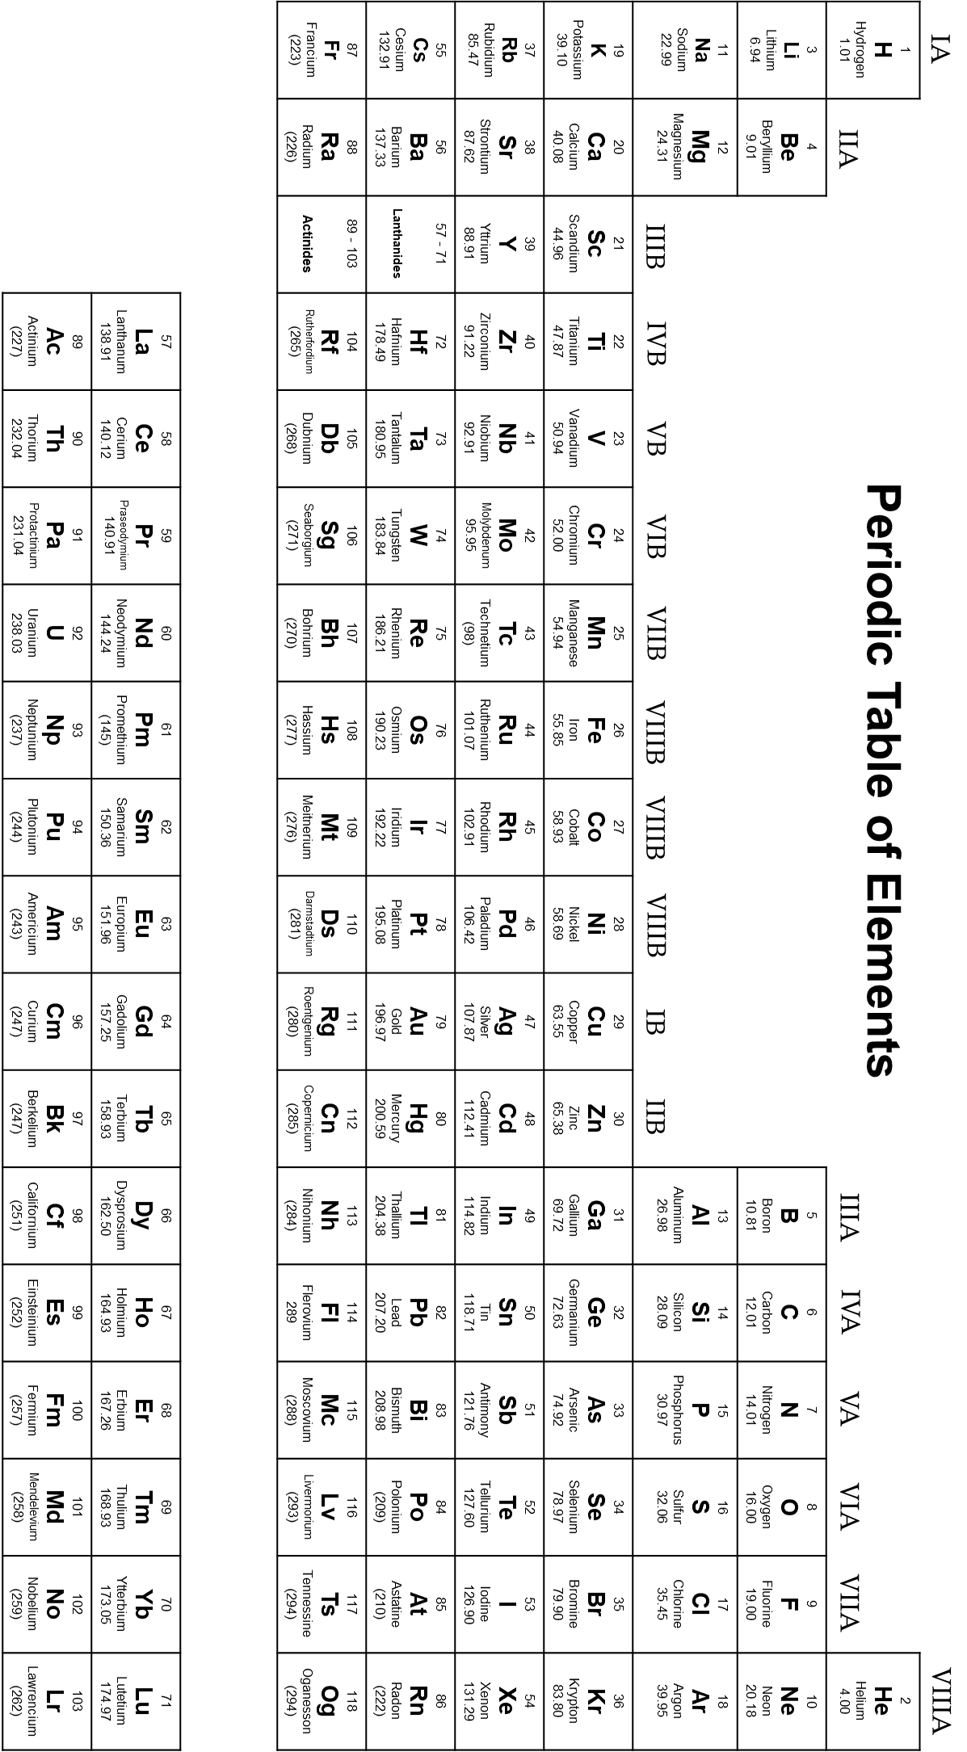
\includegraphics[width=0.75\textwidth]{periodic.png}

% ADD: Periodic Trends, Periods, Collums, Atomic Radius, Electronegativity,

\pagebreak
There is a square for each element. In the middle, you can see the atomic
symbol and the name of the element. In the upper-right corner is the
atomic number --- the number of protons in the atom.

In the upper-left corner is the atomic mass in atomic mass units.\index{atomic mass}

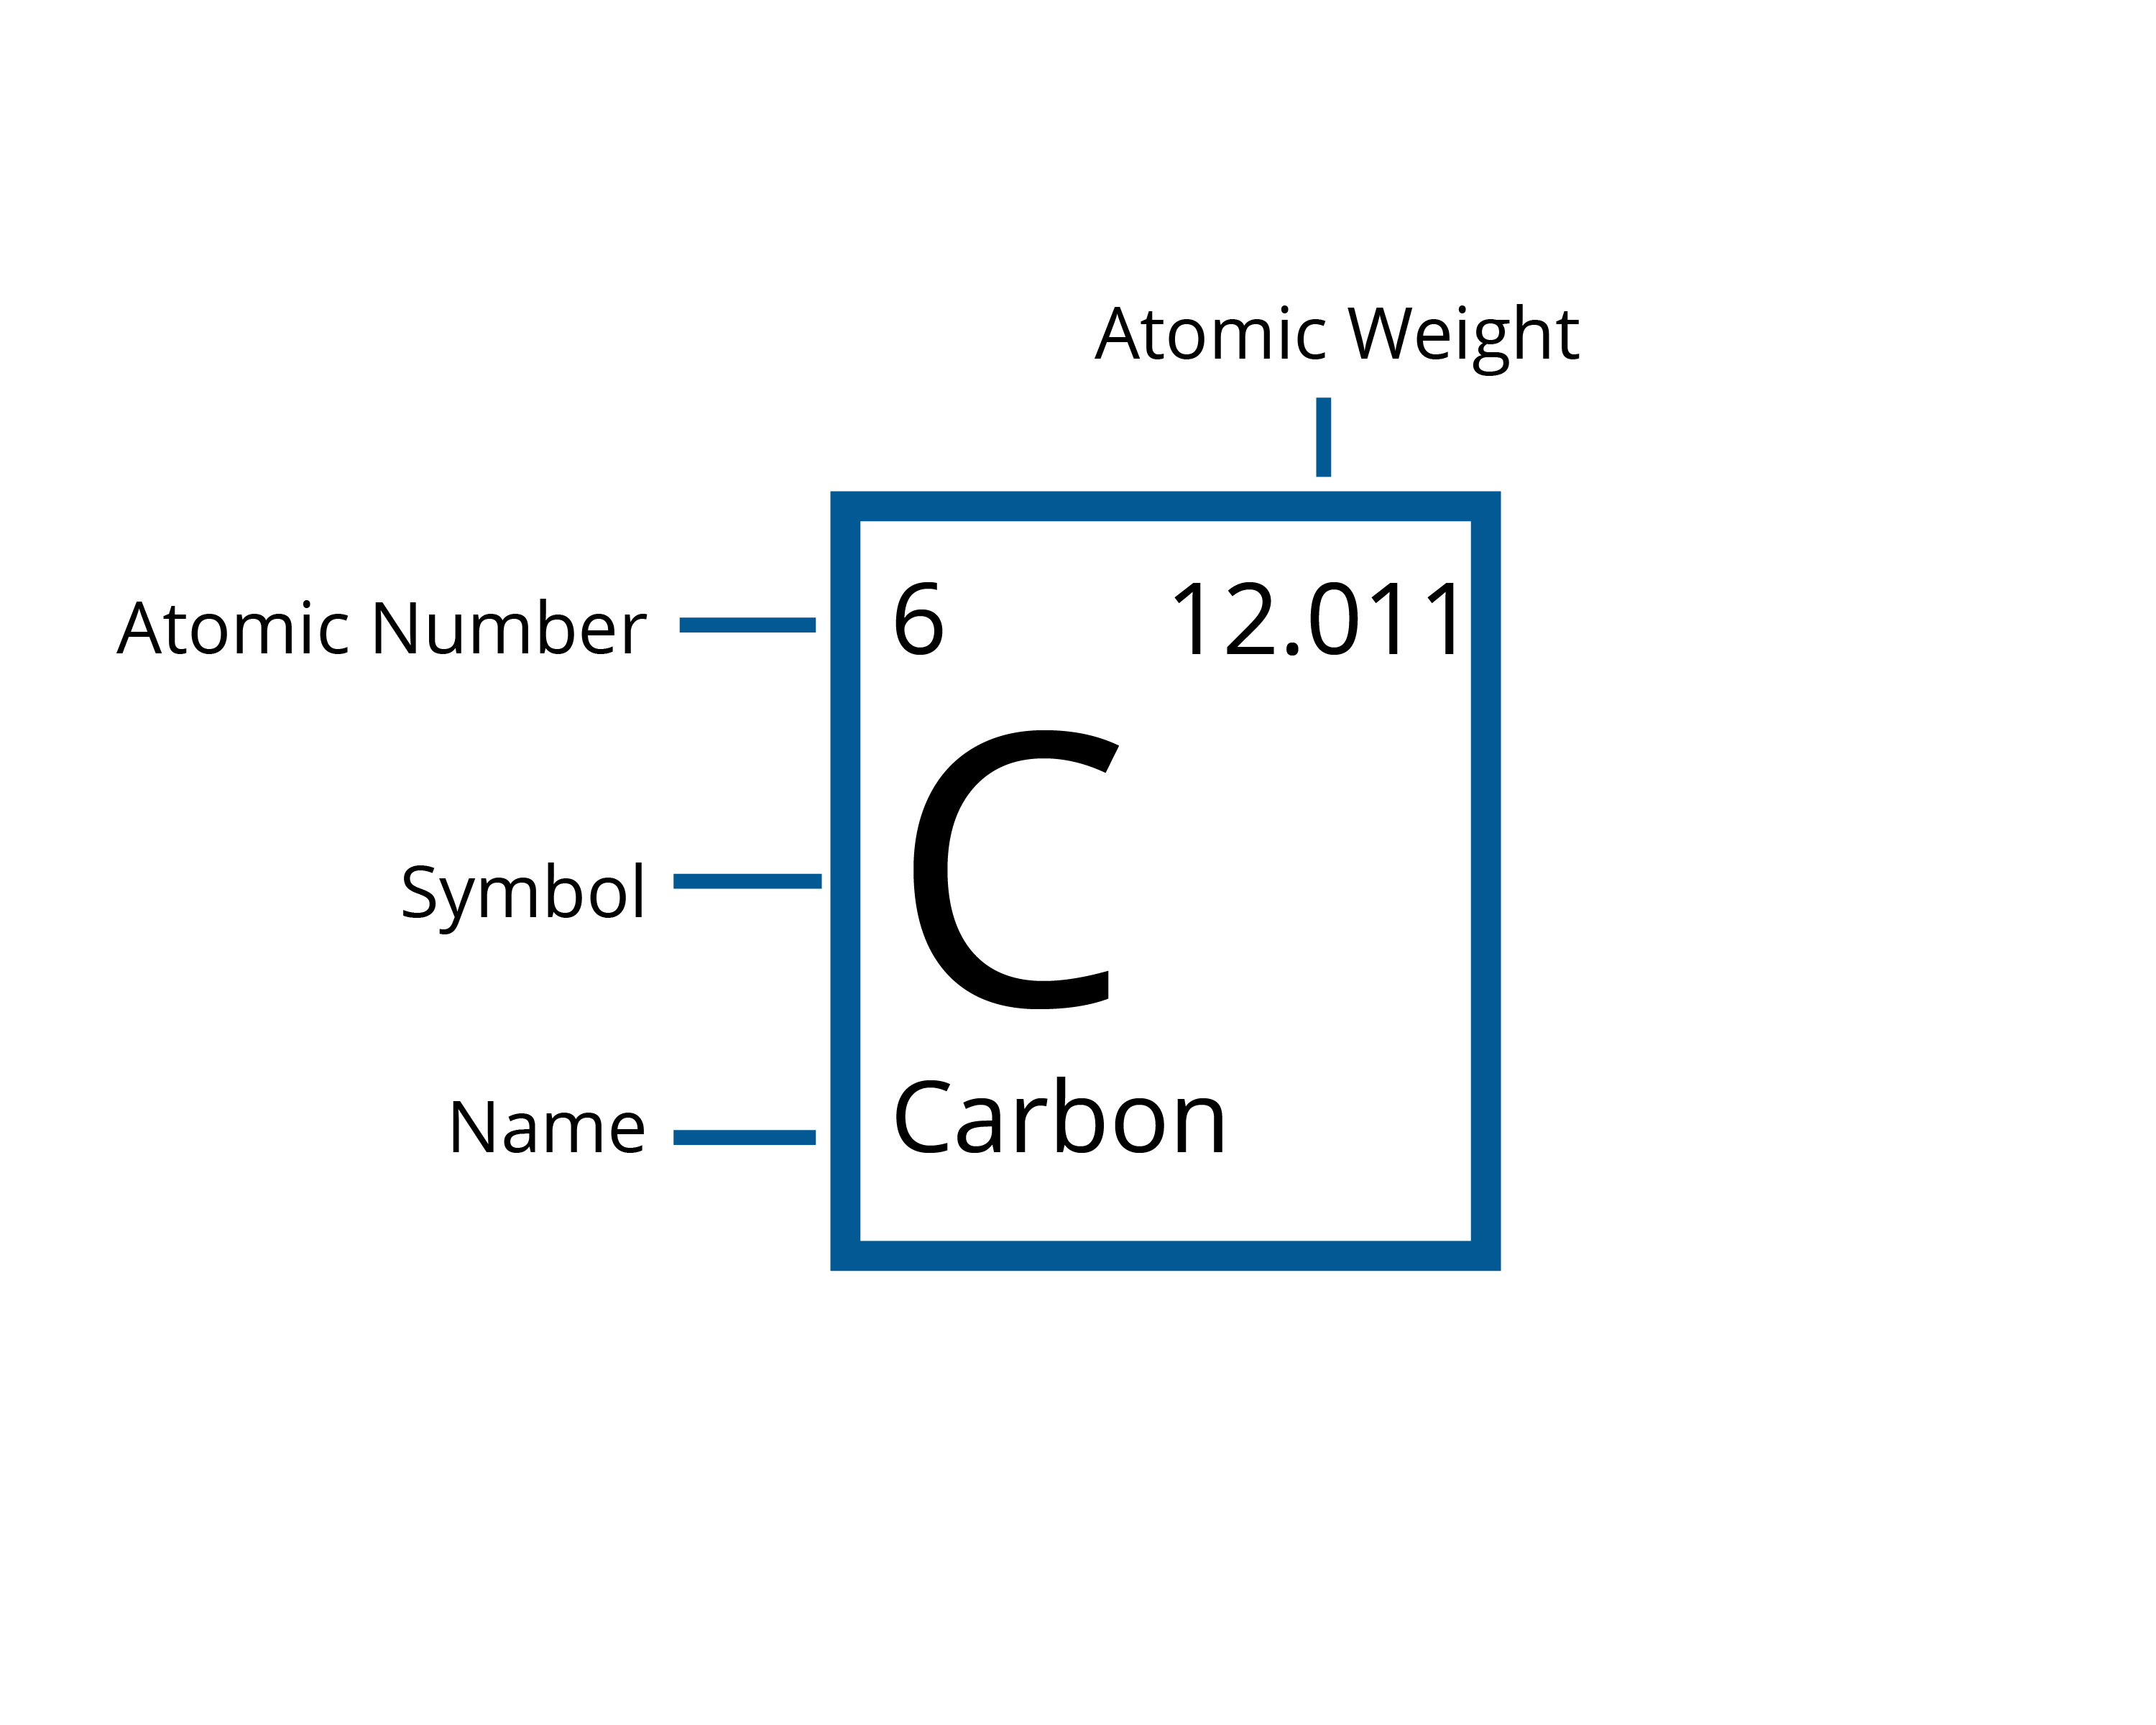
\includegraphics[width=0.8\textwidth]{element.png}

Look at the atomic mass of boron. About 80\% of all boron atoms have
six neutrons. The other 20\% have only 5 neutrons. This difference is why most boron atoms
have a mass of about 11 atomic mass units, but some have a mass of
about 10 atomic mass units. The atomic mass of boron is equivalent to the average
mass of a boron atom: 10.811.
% ADD: Talk about mass spectroscopy
%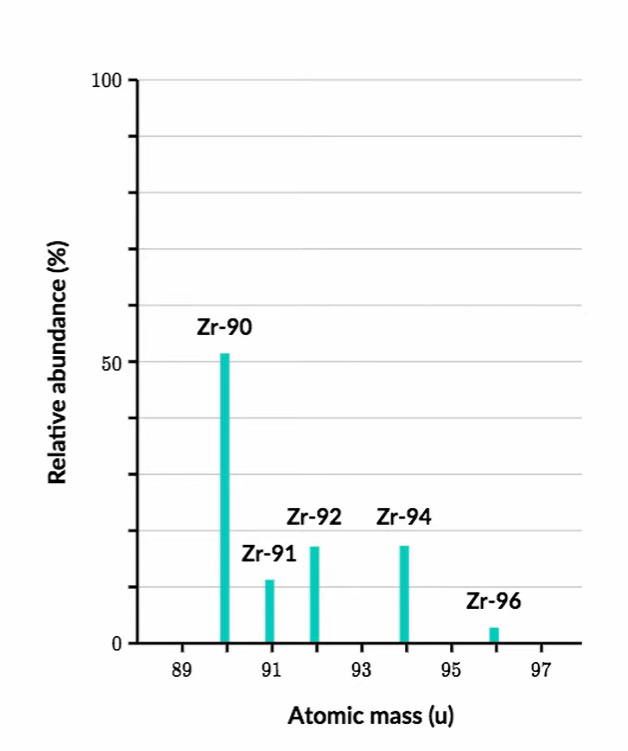
\includegraphics[width=0.75\textwidth]{KA_Mass_Spectroscopy_Zr.png}

\begin{Exercise}[title={Mass of a Water Molecule}, label=water_mass]

Using the periodic table, what is the average mass of one water molecule in atomic mass units?

\end{Exercise}
\begin{Answer}[ref=water_mass]

  The average hydrogen atom has a mass of 1.00794 atomic mass units.

  The average oxygen atom has a mass of 15.9994.

  $2 \times 1.00794 + 15.9994 = 18.01528$ atomic mass units.

\end{Answer}

\section{xfer from intro chapter} 
fixme integrate into this chapter
\subsection{Reading the Periodic Table}
The Periodic Table organizes what we know about the structure of different
elements. Each element has its own block or tile on the Periodic Table, and the
information on the tile tells us about the structure of that atom. Take a look at
the tile for carbon:

\begin{center}
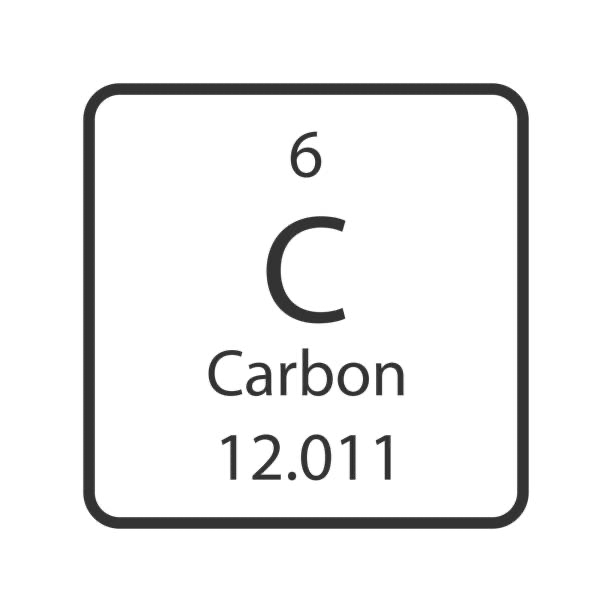
\includegraphics[width=2in]{carbon_tile.png}
\end{center}

The letter (or letters, as is the case for other elements) is the atomic symbol
for the element. There are two key numbers: the atomic number and the average
atomic mass. For carbon, the atomic number is 6 and the average atomic mass is
12.011. The atomic number tells us how many protons there are in the nucleus of
any atom of carbon. Since every element has a unique number of protons, every
element has a unique atomic number. All carbon atoms have 6 protons. The other
number is the average atomic mass - it tells us the weighted average of the
mass of all the carbons in the universe. When the average atomic mass is in
a whole number, as it is for polonium, it means that the element is very unstable.
As a result, the mass given is the mass of the most stable isotope (we'll talk
more about stability and isotopes below). On some periodic tables, the mass
number of the most stable isotope will be in parentheses or brackets. In
summary, if the larger number is a whole number, it is the mass number; if it
is a decimal (even if the decimal ends in .00), it is the average atomic mass,
which we will discuss further below.

\begin{center}
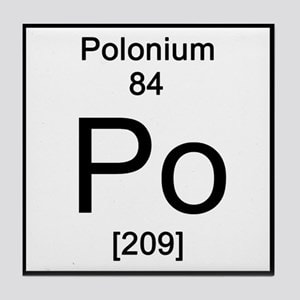
\includegraphics[width=2in]{polonium_tile.png}
\end{center}

The Royal Society of Chemistry has a very useful interactive periodic table:
periodic-table.rsc.org. We can use the periodic tile for an element to
determine the number of protons, electrons, and most common number of neutrons
for a neutral atom of that element (we'll explain why the periodic tile tells
us the "most common number of neutrons" below).

\textbf{Example}: State the atomic symbol for and the number of protons,
neutrons, and electrons in a neutral atom of plutonium.

\textbf{Solution}: The plutonium tile on your periodic table should look
something like this:
\begin{center}
   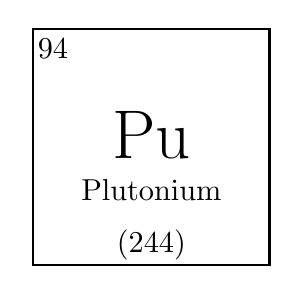
\begin{tikzpicture}
        \draw[black, thick] (-1.5, -1.5) rectangle (1.5,1.5);
        \node[font = \Huge] at (0,0.15) {Pu};
        \node[] at (-1.25, 1.25) {$94$};
        \node[] at (0, -0.55) {Plutonium};
        \node[] at (0, -1.25) {$(244)$};
    \end{tikzpicture}
\end{center}

[The information may be arranged differently, but you should at least see the
symbol and two numbers.] As you can see, the atomic symbol for plutonium is Pu.
Since its atomic number is 94, we know every atom of plutonium has 94 protons.
To know the number of electrons, we will take advantage of the fact that the
question is asking about a \textit{neutral} atom. This means there are the same
number of positive charges as negative charges. So, since there are 94 protons,
a neutral atom of plutonium must have 94 electrons (each proton has a +1 charge
and each electron has a -1 charge). Lastly, let's determine the number of
neutrons. The other number, 244, is the mass number. It represents the total
number of protons and neutrons in the nucleus. Since we know plutonium has 94
protons, we can find the number of neutrons by subtracting the atomic number
from the mass number:

\begin{center}
   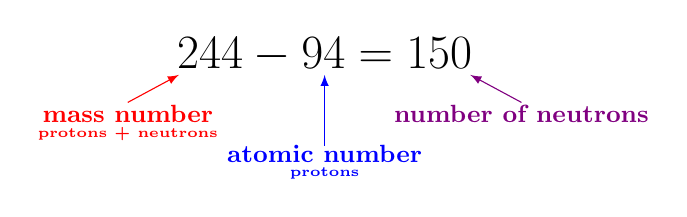
\begin{tikzpicture}
        \node[font = \LARGE] at (0,0) {$244 - 94 = 150$};
        \node[font = \small, red] at (-2.5, -0.75) {\textbf{mass number}};
        \node[font = \tiny, red] at (-2.5, -1) {\textbf{protons + neutrons}};
        \draw[red, -latex] (-2.5, -0.6) -- (-1.85, -0.25);
        \node[font = \small, blue] at (0, -1.25) {\textbf{atomic number}};
        \node[font = \tiny, blue] at (0, -1.5) {\textbf{protons}};
        \draw[blue, -latex] (0, -1.15) -- (0, -0.25);
        \node[font = \small, violet] at (2.5, -0.75) {\textbf{number of neutrons}};
        \draw[violet, -latex] (2.5, -0.6) -- (1.85, -0.25);
    \end{tikzpicture}
\end{center}

Therefore, an atom of plutonium has 150 neutrons. Now let's address how to find
the number of neutrons when the periodic tile shows an average atomic mass,
instead of a mass number. This occurs when there is more than one "version" of
an element. In the case of plutonium, there is only one version, which is why
the periodic tile shows a mass number instead of an average atomic mass. To
learn about average atomic mass, we will use carbon as an example.

Have you heard of carbon-14 dating? The phrase "carbon-14" refers to a rare
type of carbon that decays radioactively. By seeing how much carbon-14 has
decayed, scientists can estimate the age of organic materials, such as bone or
ash. Carbon-14 is a radioactive isotope (or version) of carbon. The 14 refers to
the mass number - the total amount of protons and neutrons in the nucleus
(sometimes, we shorten the isotope name by just using the atomic symbol, in
this case C-14). Isotopes are versions of an element with different numbers of
neutrons. The atomic number is the same for them all - they all have the same
number of protons. But the different number of neutrons causes different
isotopes to have different masses. Examine the models of carbon-12, carbon-13,
and carbon-14 below. What is different between them? What is the same?



You should have noticed that all three atoms have 6 protons and 6 electrons,
while they have differing numbers of neutrons. The most common isotope of carbon
is carbon-12, with 6 protons and 6 neutrons in its nucleus. Carbon-14, on the
other hand, has 8 neutrons, which makes the nucleus unstable, leading to
radioactive decay. The average atomic mass
is the weighted average of all the carbon atoms in existence. Since the vast
majority of carbon is carbon-12, the average atomic mass is very close to 12.
You cannot determine the mass number of an individual atom from the periodic
table; it only tells you the average of all the isotopes. However, especially
for light atoms (atoms in the first two rows of the periodic table), you can
usually determine the mass number of the most common isotope by rounding the
average atomic mass to the nearest whole number.

\textbf{Example}: Germanium has atomic symbol Ge. State the number of protons,
number of electrons, and most common number of neutrons in a neutral atom of
germanium.

\textbf{Solution}: Examining the periodic table, we see that germanium has an
atomic number of 32, which means a neutral atom of germanium has 32 protons and
32 electrons. The average atomic mass is 72.630, which rounds up to 73. So, the
most common isotope of germanium is Ge-73, which has $73 - 32 = 41$ neutrons.

\begin{Exercise}[title = {Determining Numbers of Subatomic Particles}, label = pne]
Use a periodic table to complete the table below (assume neutral atoms): %fixme wrap text for neutrons column

\begin{tabular}{|c|c|c|c|c|}
\hline\\
Element Name & Atomic Symbol & Protons & Most Common Number of Neutrons & Electrons\\\hline
 & Fr & & & \\\hline
 & & & & 33\\\hline
 Erbium & & & & \\\hline
  & & 48 & & \\\hline
\end{tabular}
\end{Exercise}

\begin{Answer}[ref = pne]
\begin{tabular}{|c|c|c|c|c|}
\hline\\
Element Name & Atomic Symbol & Protons & Most Common Number of Neutrons & Electrons\\\hline
 Francium & Fr & 87 & 136 & 87 \\\hline
 Arsenic & As & 33 & 42 & 33 \\\hline
 Erbium & Er & 68 & 99 & 68 \\\hline
 Cadmium & Cd & 48 & 64 & 48 \\\hline
\end{tabular}
\end{Answer}




\section{Heavy atoms aren't stable}

When you look at the periodic table, there are a surprisingly large
number of elements. You might be told to ``Drink milk so that you can
get the calcium you need.'' However, no one has told you ``You should
eat kale so that you get enough copernicium in your diet.''

Copernicium, with 112 protons and 173 neutrons, has only been observed
 in a lab. It is highly radioactive and unstable (meaning it decays). A copernicium
atom usually lives for less than a minute before decaying.
% ADD: Half Life

The largest stable element is lead, which has 82 protons and between
122 and 126 neutrons. Elements with lower atomic numbers than lead,
have at least one stable isotope, while elements with higher atomic numbers
than lead don't.

Bismuth, with an atomic number of 83, is \textit{almost} stable. In fact, most
bismuth atoms will live for billions of years before decaying!

\graphicspath{{../../Chapters/work_energy/en_US}}
\chapter{Work and Energy}

In this chapter, we are going to talk about how engineers define work
and energy. It frequently takes force to get work done. Let's start with thinking about the relationship between force and energy. As we learned earlier, Force is measured in
newtons, and one newton is equal to the force necessary to accelerate one
kilogram at a rate of $1 m/s^2$.

When you lean on a wall, you are exerting a force on the wall, but you
aren't doing any work. On the other hand, if you push a car for a mile,
you are clearly doing work. Work, to an engineer, is the force you
apply to something, as well as the distance that it moves, in the direction
of the applied force. We measure work in \textit{joules}. A joule is one
newton of force over one meter.\index{Joule}

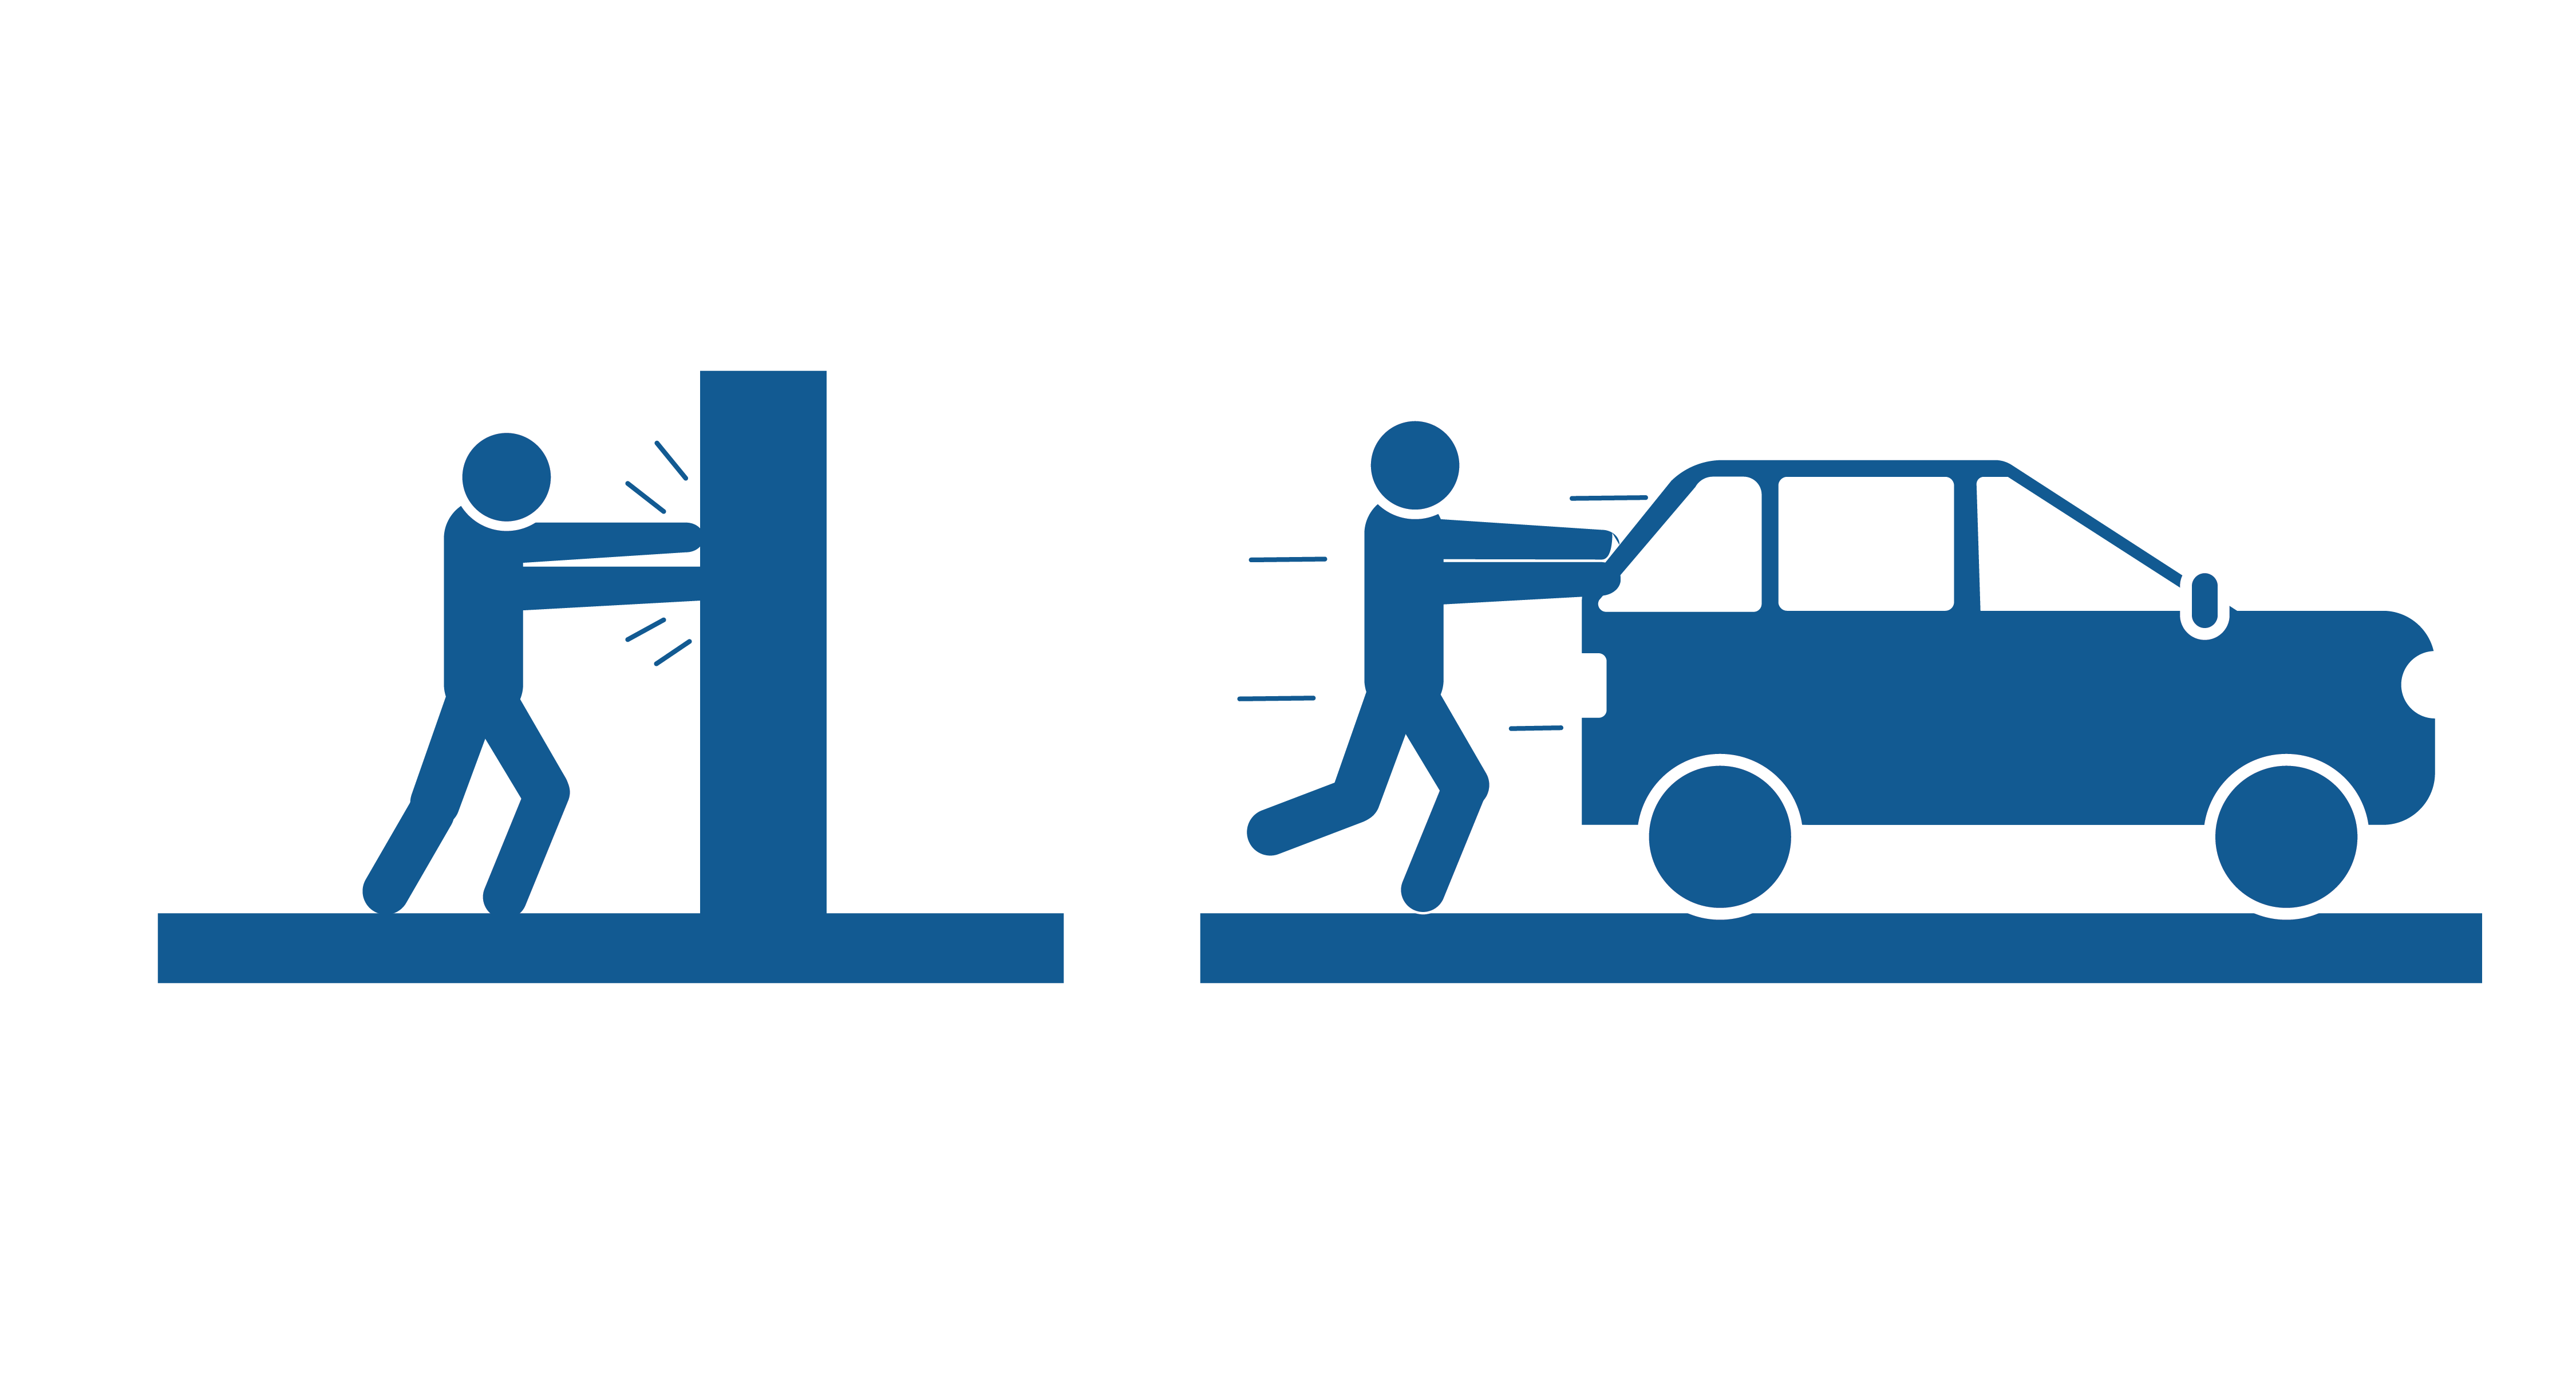
\includegraphics[width=1\textwidth]{workvsforce.png}

For example, if you push a car uphill with a force of 10 newtons for 12
meters, you have done 120 joules of work.\index{work}
% ADD: We can represent this with the equations, Work Energy Therom

Work is how energy is transferred from one thing to another. When you
push the car, you also burn sugars(energy of the body) in your blood. That energy is then
transferred to the car: after it has been pushed uphill.

Thus, we measure the energy something consumes or generates in 
units of work: joules, kilowatt-hours, horsepower-hours, foot-pounds,
BTUs( British Thermal Unit), and calories.

Let's go over a few different forms that energy can take.

Watch Khan Academy's \textbf{Changes in energy} at \url{https://www.khanacademy.org/science/ms-physics/x1baed5db7c1bb50b:energy/x1baed5db7c1bb50b:changes-in-energy/a/changes-in-energy}

\section{Forms of Energy}\index{energy!Forms of}

In this section we are going to learn about several different types of energy:
\begin{itemize}
\item Heat
\item Chemical Energy
\item Kinetic Energy
\item Gravitational Potential Energy
\end{itemize}

\subsection{Heat}\index{heat}

When you heat something, you are transferring energy to it. The BTU
 is a common unit for heat: One BTU is the
amount of heat required to raise the temperature of one pound of water,
by one degree. One BTU is about 1,055 joules. In fact, when you buy and sell
natural gas as fuel, it is priced by the BTU.\index{heat} \index{BTU}

\subsection{Electricity}\index{electricity}

Electricity is the movement of electrons. When you push electrons
through a space that resists their passage (like a light bulb),
energy is transferred from the power source ( a battery)
 into the source of the resistance.

Let's say your lightbulb consumes 60 watts of electricity, and you leave it on for 24 hours.
We would say that you have consumed 1.44 kilowatt hours or 3,600,000 joules.

Watch Khan Academy's \textbf{Introduction to charge} at \url{https://www.khanacademy.org/science/in-in-class10th-physics/in-in-electricity/in-in-electric-current-circuit/v/intro-to-charge}

\subsection{Chemical Energy}\index{chemical energy}

As mentioned early, some chemical reactions consume energy and some
produce energy. Thus, energy can be stored in the structure of a
molecule. When a plant uses photosynthesis to rearrange water and
carbon dioxide into a sugar molecule, it converts the energy in
the sunlight( solar energy) into chemical energy. Remember photosythesis is a process that releases energy.
Therefore, the sugar molecule has more chemical energy than the carbon dioxide and water molecules that were
used in its creation.
% ADD: photosythesis equation 
% KA: https://www.khanacademy.org/science/ap-biology/cellular-energetics/photosynthesis/a/intro-to-photosynthesis

In our diet, we measure this energy in \textit{kilocalories}. A
calorie is the energy necessary to raise one gram of water one degree
Celsius: it is about 4.19 joules. This is a very small unit: an apple
has about 100,000 calories( 100 kilocalories), so people working with food started
measuring everything in kilocalories.\index{calories}
% ADD: Conversion chapter should come before this chapter

Here is where things get confusing: People who work with food got tired of
saying ``kilocalories'', so they just started using ``Calorie'' to
mean 1,000 calories.  This has created terrible confusion over the
years. So if the C is capitalized, ``Calorie'' probably means kilocalorie.

\subsection{Kinetic Energy}\index{kinetic energy}

A mass in motion has energy. For example, if you are in a moving car
and you slam on the breaks, the energy from the motion of the
car will be converted into heat in the breaks and under the tires.

How much energy does the car have?
% ADD: section specifically about KE AND U, use roller coaster diagram

\begin{mdframed}[style=important, frametitle={Formula for Kinetic Energy}]

$$E = \frac{1}{2} m v^2$$

where $E$ is the energy in joules, $m$ is the mass in kilograms, and
$v$ is the speed in meters per second.

\end{mdframed}

\subsection{Gravitational Potential Energy}\index{potential energy!gravitational}

Watch Khan Academy's \textbf{Potential energy} at \url{https://youtu.be/oGzwVYPxKjg}

When you lift something heavy onto a shelf, you are giving it
\textit{potential energy}. The amount of energy that you transferred
to it is proportional to its weight and the height that you lifted it.

On the surface of the earth, gravity will accelerate a heavy object downward at
a rate of $9.8 m/s^2$.

\begin{mdframed}[style=important, frametitle={Formula for Gravitational Potential Energy}]
On earth, then, gravitational potential energy is given by

$$E = (9.8)mh$$


where $E$ is the energy in joules, $m$ is the mass of the object you
lifted, and $h$ is the height that you lifted it.

\end{mdframed}


There are other kinds of potential energy. For example, when you draw
a bow, you have given that bow potential energy. When you release it,
the potential energy is transferred to the arrow, which expresses it
as kinetic energy.
% ADD: section about KE and U

\section{Conservation of Energy}

The first law of thermodynamics says ``Energy is neither created nor
destroyed.''\index{energy!conservation of}

Energy can change forms: Your cells consume chemical energy to give
gravitational potential energy to a car you push up a hill. However, the total amount of
energy in a closed system stays constant.
% ADD: Create Systems chapter before introducing concept here

\begin{Exercise}[title={The Energy of Falling}, label=energy_falling]
  
A 5 kg cannonball falls off the top of a 3 meter ladder. Just before
it hits the floor, all of its gravitational potential energy has been
converted into kinetic energy.  How fast is the cannonball going when
it hits the floor?

\end{Exercise}
\begin{Answer}[ref=energy_falling]

  At the top of the ladder, the cannonball has $(9.8)(5)(3) = 147$ joules of potential energy.

  At the bottom, the kinetic energy $\frac{1}{2}(5)v^2$ must be equal
  to 147 joules. So $v^2 = \frac{294}{5}$.  Thus it is going about
  $7.7$ meters per second.

  (Yes, a tiny amount of energy is lost to air resistance. For a dense
  object moving at these relatively slow speeds, this energy is
  neglible.)
  
\end{Answer}


\section{Efficiency}


Watch Khan Academy's \textbf{Laws of thermodynamics} at \url{https://www.khanacademy.org/science/ap-biology/cellular-energetics/cellular-energy/a/the-laws-of-thermodynamics}

Although energy is always conserved as it moves through different
forms, scientists aren't always that good at controlling it.\index{efficiency}

For example, a car engine consumes the chemical energy in gasoline. Only
about 20\% of the energy consumed is used to turn the wheels.  Most of
the energy is actually lost as heat. If you run a car for a while, the engine
gets very hot and the exhaust going out the tailpipe turns hot.

A human is about 25\% efficient. Most of the loss is in the heat produced
during the chemical reactions that turns food into motion.
% ADD: Cellular Respiration
 
In general, if you are trying to increase efficiency in any system,
the solution is usually easy to identify because heat is produced. Reduce heat, Increase efficiency.

Light bulbs are an interesting case. To get the light of a 60 watt
incandescent bulb, you can use an 8 watt LED or a 16 watt fluorescent
light. Thus, we say that the LED light is much more efficient: If you
run both, the incandescent bulb will consume 1.44 kilowatt-hours. The
LED will consume only 0.192 kilowatt-hours.

Besides light, the incandescent bulb is producing a lot of heat. If it
is inside your house, what happens to the heat? It warms your house.

In the winter, when you want light and heat, the incandescent bulb is
100\% efficient!

In the summer, if you are running the air conditioner, the
incandescent bulb is worse than just ``inefficient at making light'' --
it is actually counteracting the air conditioner! 


\graphicspath{{../../Chapters/units_conversions/en_US}}
\chapter{Units and Conversions}

At this point, you are working with a lot of units: grams for weight,
joules for energy, newtons for force, meters for distance, seconds for
time, etc. For each type of measurement, there are several different
units; for example, distance can be measured in feet, miles,
and light-years.

\begin{mdframed}[style=important, frametitle={Some Equalencies}]

\begin{tabular}{r | l}
  \hline
  \multicolumn{2}{c}{\textbf{Distance}}\\
  1 mile & 1.6093 kilometers \\
  1 foot & 0.3048 meters \\
  1 inch & 2.54 centimeters \\
  1 light-year & $9.461 \times 10^{12}$ kilometers\\
  \hline
  \multicolumn{2}{c}{\textbf{Volume}}\\
  1 milliliter & 1 cubic centimeter \\
  1 quart & 0.9461 liters \\
  1 gallon & 3.7854 liters \\
  1 fluid ounce & 29.6 milliliters \\
  \hline
  \multicolumn{2}{c}{\textbf{Mass}}\\
  1 pound & 0.4535924 kilograms\\
  1 ounce & 0.4535924 grams\\
  1 metric ton & 1000 kilograms \\
  \hline
  \multicolumn{2}{c}{\textbf{Force}}\\
  1 newton & 1 kilogram meter per sec$^2$\\
  \hline
  \multicolumn{2}{c}{\textbf{Pressure}}\\
  1 pascal & 1 newton per square meter \\
  1 bar & 0.98692 atmosphere \\
  1 pound per square inch & 6897 pascals \\
  \hline
  \multicolumn{2}{c}{\textbf{Energy}}\\
  1 joule & 1 newton meter \\
  1 calorie & 4.184 joules \\
  1 kilowatt-hour & $3.6 \times 10^{6}$ joules  \\
\end{tabular}\index{units table}

(You don't need to memorize these! Just remember that this page is here.)
% Suggest putting this in the front or back of the book, maybe create a print out

\end{mdframed}

In the metric system, prefixes are often used to express a multiple. Here are the common prefixes:\index{metric system!prefixes}

\begin{mdframed}[style=important, frametitle={Common Prefixes for Metric Units}]

\begin{tabular}{r | l}
giga  & $\times 10^{9}$\\
mega  & $\times 10^{6}$\\
kilo  & $\times 10^{3}$\\
milli  & $\div 10^{3}$\\
micro  & $\div 10^{6}$\\
nano  & $\div 10^{9}$\\
\end{tabular}

(These are worth memorizing. Here's a mnemonic: ``King Henery Doesn't Usually Drink Chocolate Milk.'')
\end{mdframed}

\section{Conversion Factors}

Here is a really handy trick to remembering how to do conversions
between units.\index{conversion factors}

Often, you will be given a table like the one above, and someone will ask you
``How many miles are in 0.23 light-years?''  You know that 1 mile = 1.6093
kilometers and that 1 light-year is $9.461 \times 10^{12}$ kilometers.
How do you do the conversion?

The trick is to treat the two parts of the equality as a fraction that equals 1.  That is, you think:

$$\frac{1 \text{ miles}}{1.6093 \text{ km}} = \frac{1.6093 \text{ km}}{1 \text{ miles}} = 1$$

and

$$\frac{1 \text{ light-years}}{9.461 \times 10^{12} \text{ km}} = \frac{9.461 \times 10^{12} \text{ km}}{1 \text{ light-years}} = 1$$

We call these fractions \textit{conversion factors}.

Now, your problem is

$$0.23 \text{ light-years} \times \textit{ Some conversion factors} = ? \text{ miles}$$

Note that when you multiply fractions together, things in the numerators can cancel with things in the denominator:

$$\left( \frac{31\pi}{47} \right) \left( \frac{11}{37\pi}\right) = \left(\frac{31\cancel{\pi}}{47}\right) \left( \frac{11}{37\cancel{\pi}}\right) = \left(\frac{31}{47} \right) \left( \frac{11}{37} \right)$$

When working with conversion factors, you will do the same with the units:

\begin{multline*}
  0.23 \text{ light-years} \left( \frac{9.461 \times 10^{12} \text{ km}}{1 \text{ light-years}} \right) \left( \frac{1 \text{ miles}}{1.6093 \text{ km}} \right) = \\
  0.23 \text{ \cancel{light-years}} \left( \times \frac{9.461 \times 10^{12} \text{ \cancel{km}}}{1 \text{ \cancel{light-years}}} \right) \left( \frac{1 \text{ miles}}{1.6093 \text{ \cancel{km}}}\right) = \frac{(0.23)(9.461 \times 10^{12})}{1.6093} \text{ miles}$$
\end{multline*}

\begin{Exercise}[title={Simple Conversion Factors}, label=simple_conversion_factors]

  How many calories are in 4.5 kilowatt-hours?
  
\end{Exercise}
\begin{Answer}[ref=simple_conversion_factors]

  $$4.5 \text{ \cancel{kWh}} \left( \frac{3.6 \times 10^{6} \text{ \cancel{joules}}}{1 \text{ \cancel{kWh}}} \right) \left( \frac{1 \text{ calories}}{4.184 \text{ \cancel{joules}}}\right) = \frac{(4.5)(3.6 \times 10^6)}{4.184} = 1.08 \times 10^6 \text {calories}$$
  
\end{Answer}

\section{Conversion Factors and Ratios}

Conversion factors also work on ratios.  For example, if you are told
that a bug is moving 0.5 feet every 120 milliseconds. What is that in
meters per second?

The problem then is

$$\frac{0.5 \text{ feet}}{120 \text{ milliseconds}} = \frac{\text{? m}}{second}$$

So you will need conversion factors to replace the ``feet'' with ``meters'' and to replace ``milliseconds'' with ``seconds'':

\begin{multline*}
\left(\frac{0.5 \text{ \cancel{feet}}}{120 \text{ \cancel{milliseconds}}}\right) \left( \frac{0.3048 \text{ meters}}{1 \text{ \cancel{feet}}} \right) \left( \frac{ 1000 \text{ \cancel{milliseconds}}} {1 \text{ second}}\right) = \frac{(0.5)(0.3048)(1000)}{120}\text{ m/second}
\end{multline*}

\begin{Exercise}[title={Conversion Factors}, label=conversion_factors]

The hole in the bottom of the boat lets in 0.1 gallons every 2 minutes.  How many milliliters per second is that?
  
\end{Exercise}
\begin{Answer}[ref=onversion_factors]

  \begin{multline*}
    \frac{0.1 \text{ \cancel{gallons}}}{2 \text{ \cancel{minutes}}}
  \left( \frac{3.7854 \text{ \cancel{liters}}}{1 \text{ \cancel{gallons}}} \right)
  \left( \frac{1000 \text{ milliliters}}{1\text{ \cancel{liters}}}\right)
  \left( \frac{1 \text{ \cancel{minutes}}}{60 \text{ seconds}} \right) = \\
  \frac{(0.1)(3.7854)(1000)}{(2)(60)} \text{ ml/second} = 3.1545 \text{ ml/second}
  \end{multline*}
  
\end{Answer}

\section{When Conversion Factors Don't Work}

Conversion factors only work when the units being converted are
proportional to each other. Gallons and liters, for example, are
proportional to each other: If you have $n$ gallons, you have $n
\times 3.7854$ liters.

Degrees celsius and degrees farenheit are \textit{not} proportional to
each other.  If your food is $n$ degrees celsius, it is $n \times
\frac{9}{5} + 32$ degrees farenheit.  You can't use conversion factors
to convert celsius to farenheit.

Watch Khan Academy's video on this at \url{https://www.khanacademy.org/test-prep/sat/x0a8c2e5f:untitled-652/x0a8c2e5f:problem-solving-and-data-analysis-lessons-by-skill/a/gtp--sat-math--article--units--lesson}


\graphicspath{{../../Chapters/simple_machines/en_US}}
\chapter{Simple Machines}

As mentioned earlier, physicists define work as the force applied times the distance over which it is applied. For example, if you push your car 100 meters with a force of 17 newtons, you have done 1700 joules of work.

Humans have long needed to move heavy objects, so many centuries ago, we developed simple machines to reduce the amount of force necessary to perform such tasks. These include:

\begin{itemize}
    \item Levers
    \item Pulleys
    \item Inclined planes
    \item Gears
    \item Hydraulics
    \item Screws
\end{itemize}

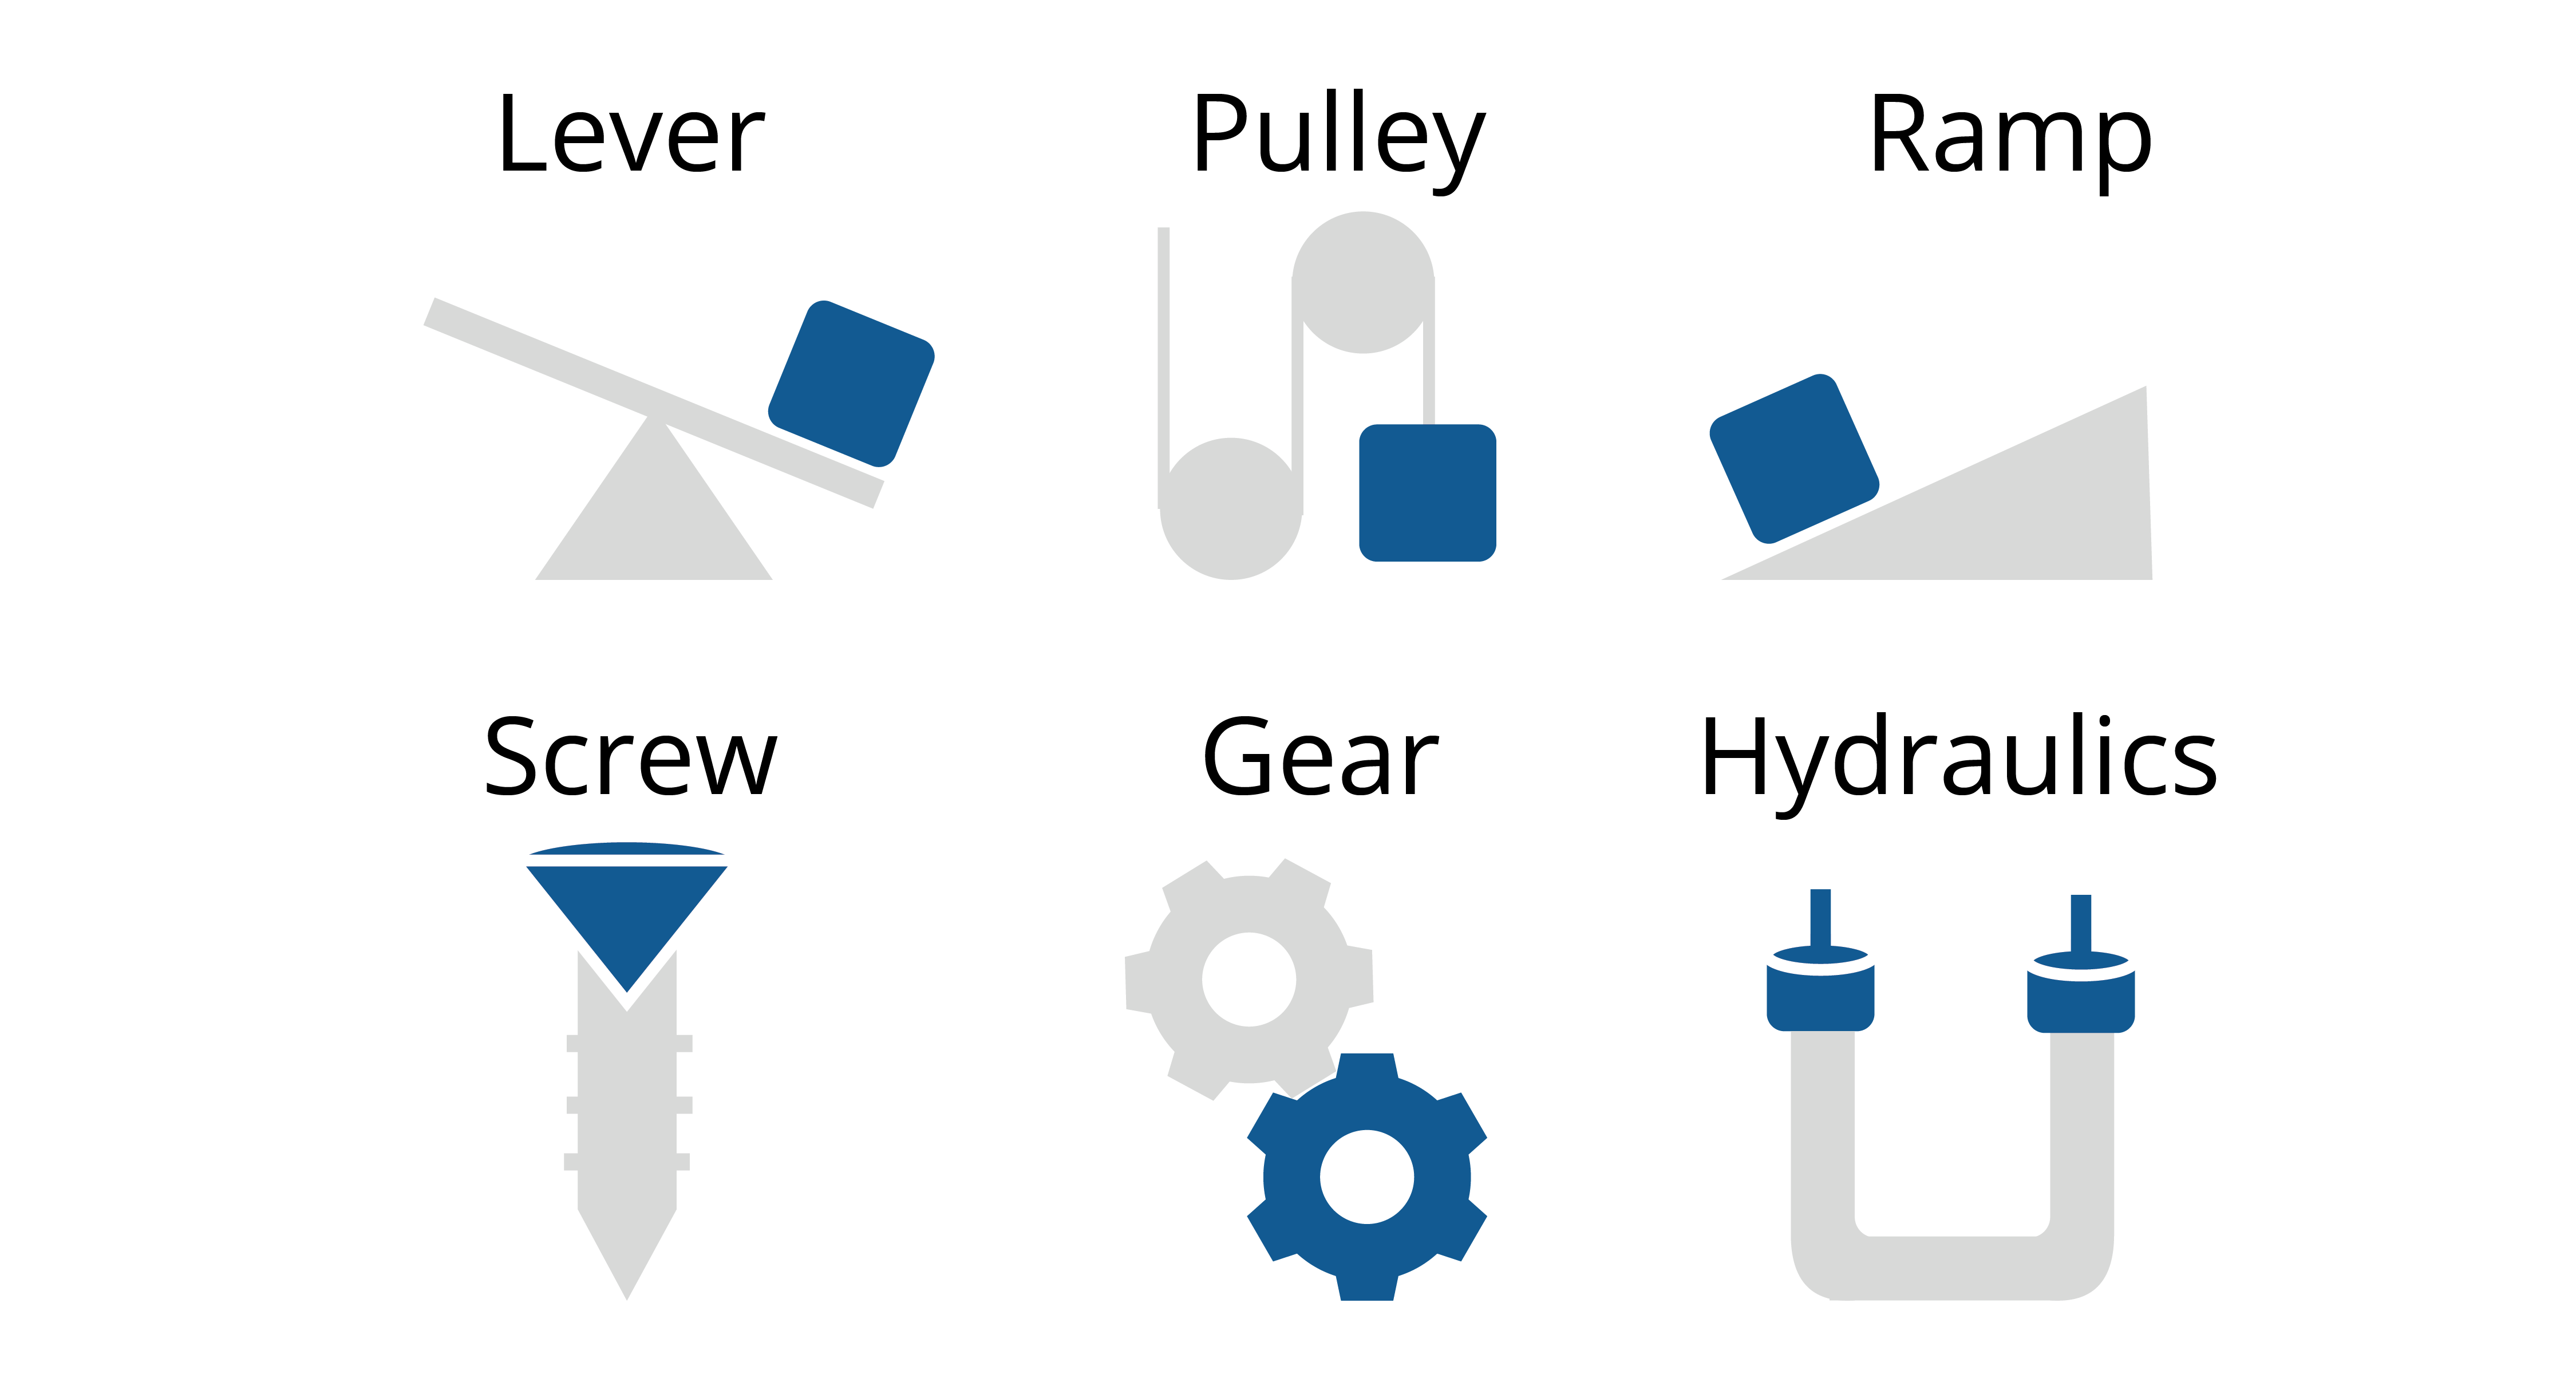
\includegraphics[width=\textwidth]{simplemachines.png}

While these machines can reduce the force needed, they do not change the total amount of work that must be done. For instance, if the force is reduced by a factor of three, the distance over which the force must be applied increases by the same factor.

The term \textit{mechanical advantage} refers to the increase in force achieved by using these machines.

\section{Levers}

A lever pivots on a fulcrum. To decrease the necessary force, the load is placed closer to the fulcrum than where the force is applied.

Physicists also discuss the concept of \newterm{torque} created by a force. When you apply force to a lever, the torque is the product of the force you exert and the distance from the point of rotation.

Torque is typically measured in newton-meters.

To balance two torques, the products of force and distance must be equal. Thus, assuming the forces are applied in the correct direction, the equation becomes:

\[
R_L F_L = R_A F_A
\]

where \( R_L \) and \( R_A \) represent the distances from the fulcrum to where the load’s force and the applied force are exerted, respectively, and \( F_L \) and \( F_A \) are the magnitudes of the forces.

\begin{Exercise}[title={Lever}, label=lever]
Paul, who weighs 70 kilograms, sits on a see-saw 4 meters from the fulcrum. Jan, who weighs 50 kilograms, wishes to balance the see-saw. How far should Jan sit from the fulcrum?
\end{Exercise}
\begin{Answer}[ref=lever]
Paul exerts a force of \( 70 \times 9.8 = 686 \) newtons at a distance of 4 meters from the fulcrum, creating a torque of \( 686 \times 4 = 2744 \) newton-meters. Jan exerts a force of \( 50 \times 9.8 = 490 \) newtons.

Let \( r \) be the distance from the fulcrum to Jan's seat. To balance the torques:

\[
490 \times r = 2744
\]

Solving for \( r \), we find \( r = \frac{2744}{490} \approx 5.6 \) meters.
\end{Answer}

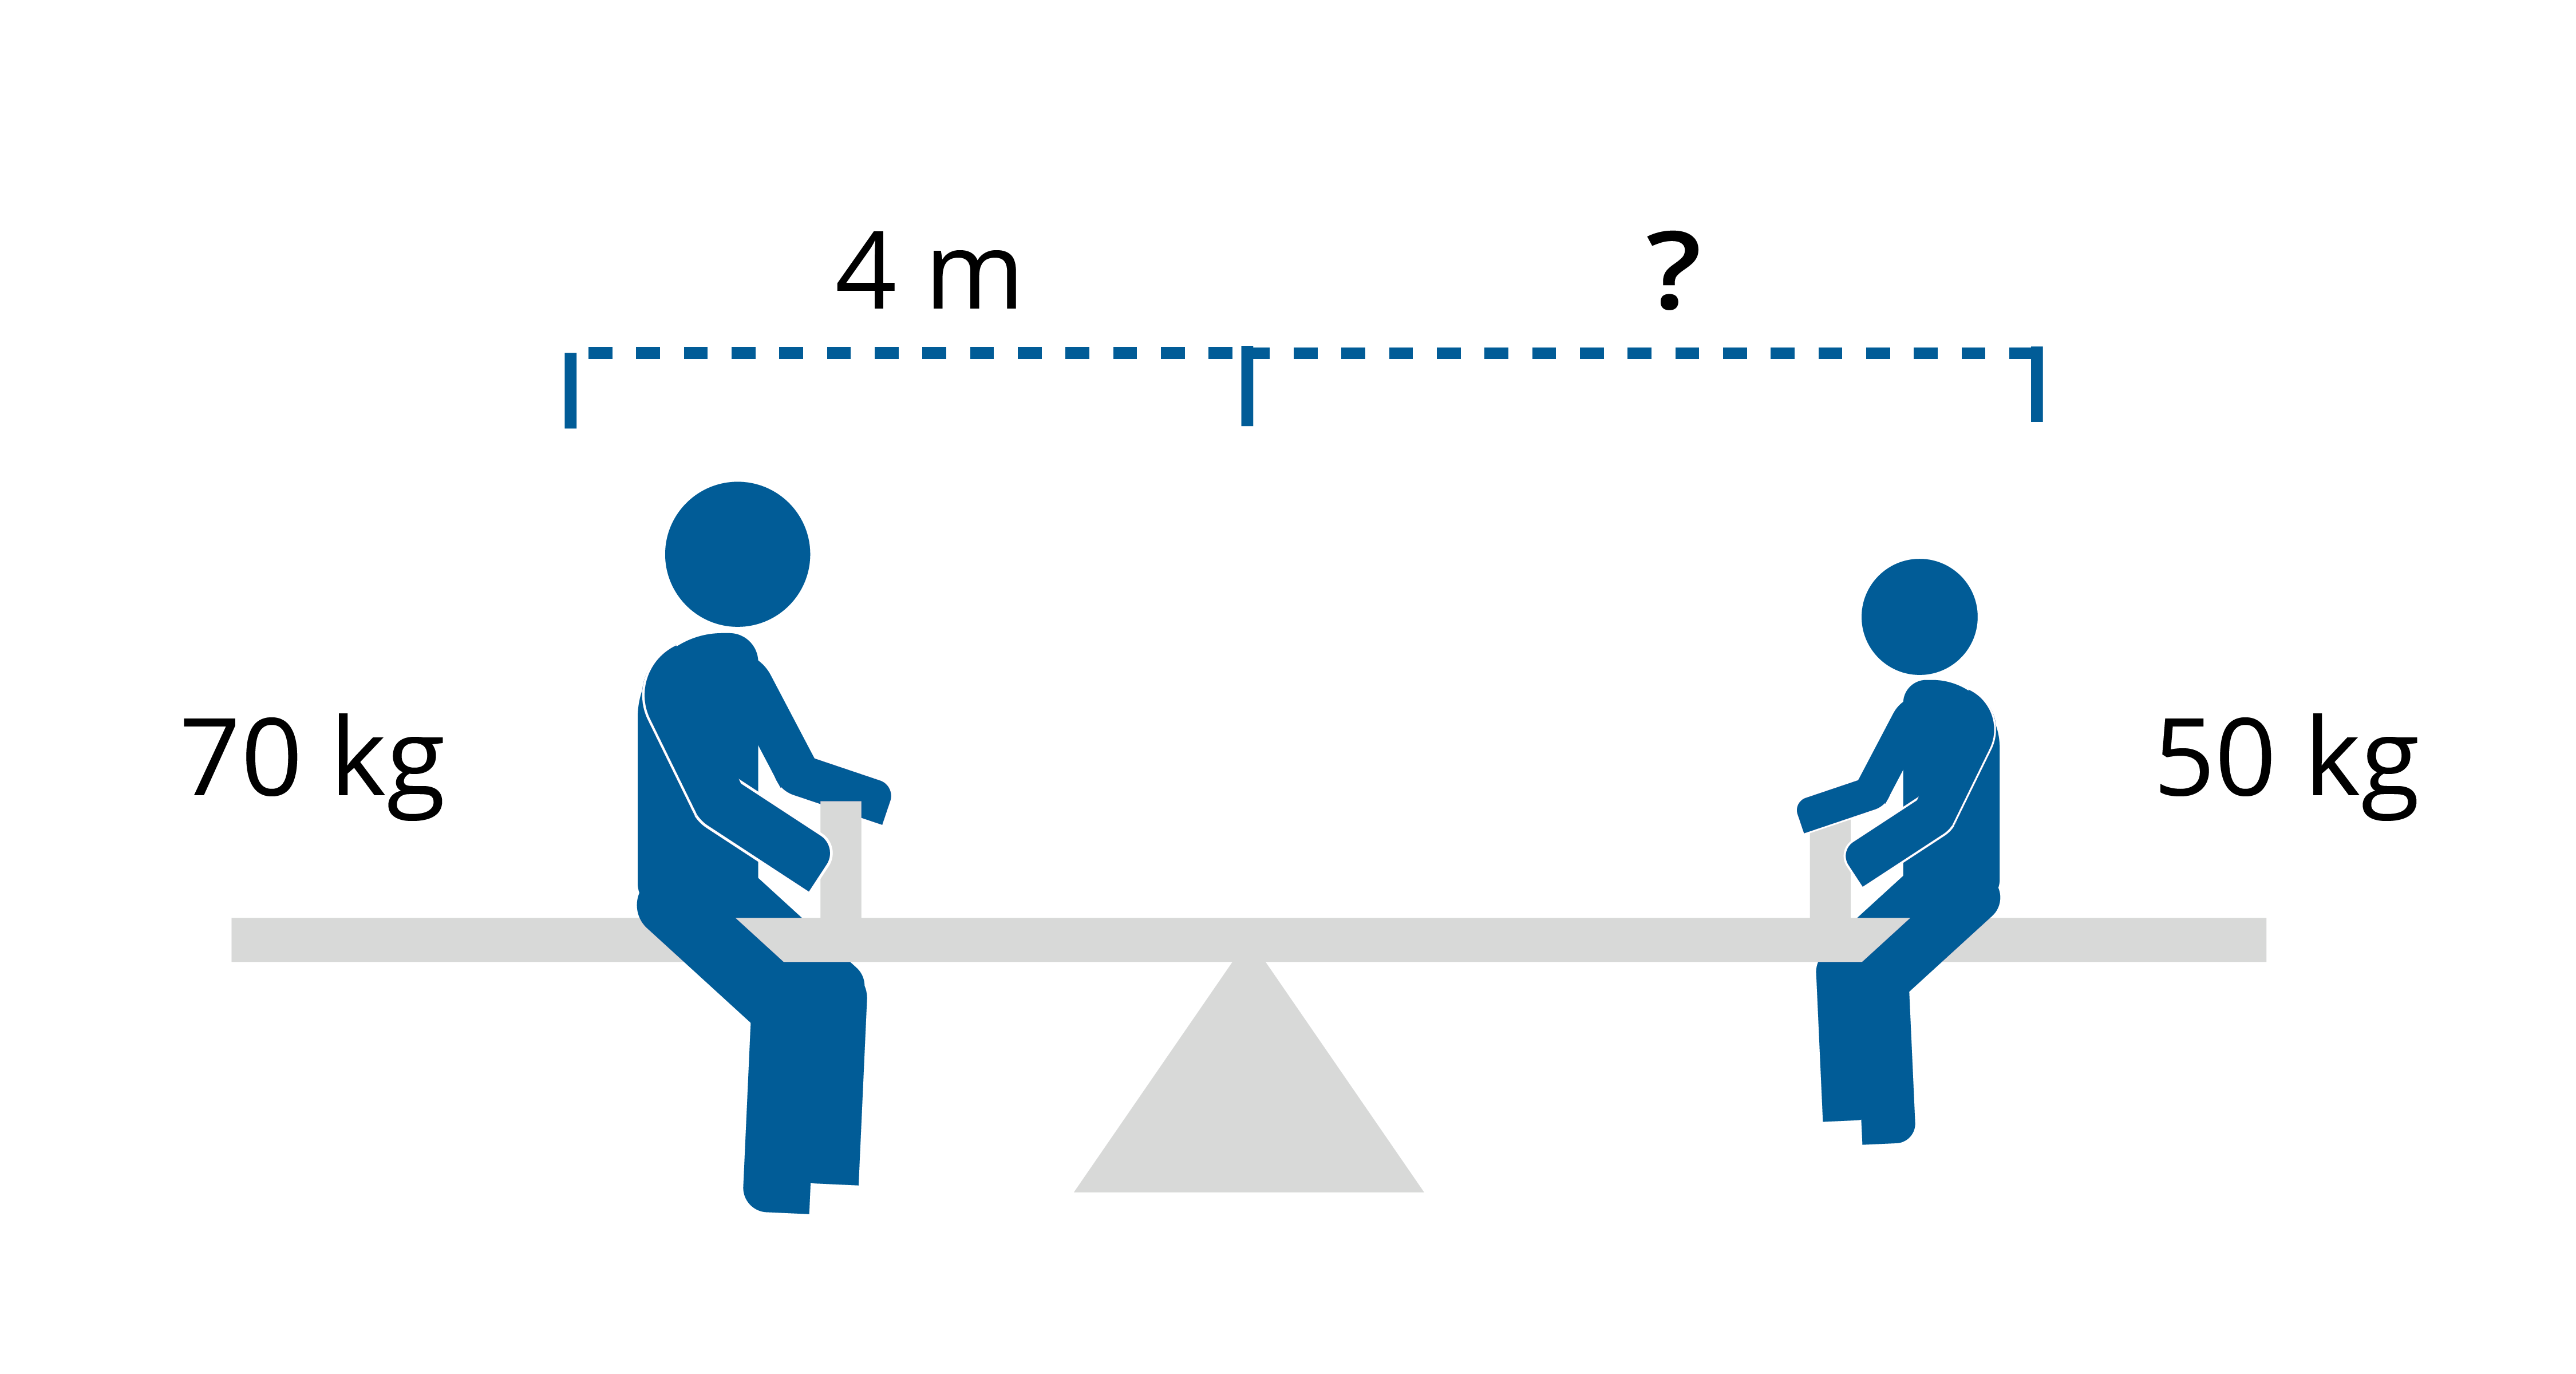
\includegraphics[width=0.6\textwidth]{seesaw.png}

\section{Inclined Planes}

Inclined planes, or ramps, allow you to roll or slide objects to a higher level. Steeper ramps require less mechanical advantage. For instance, it is much easier to roll a ball up a wheelchair ramp than a skateboard ramp.

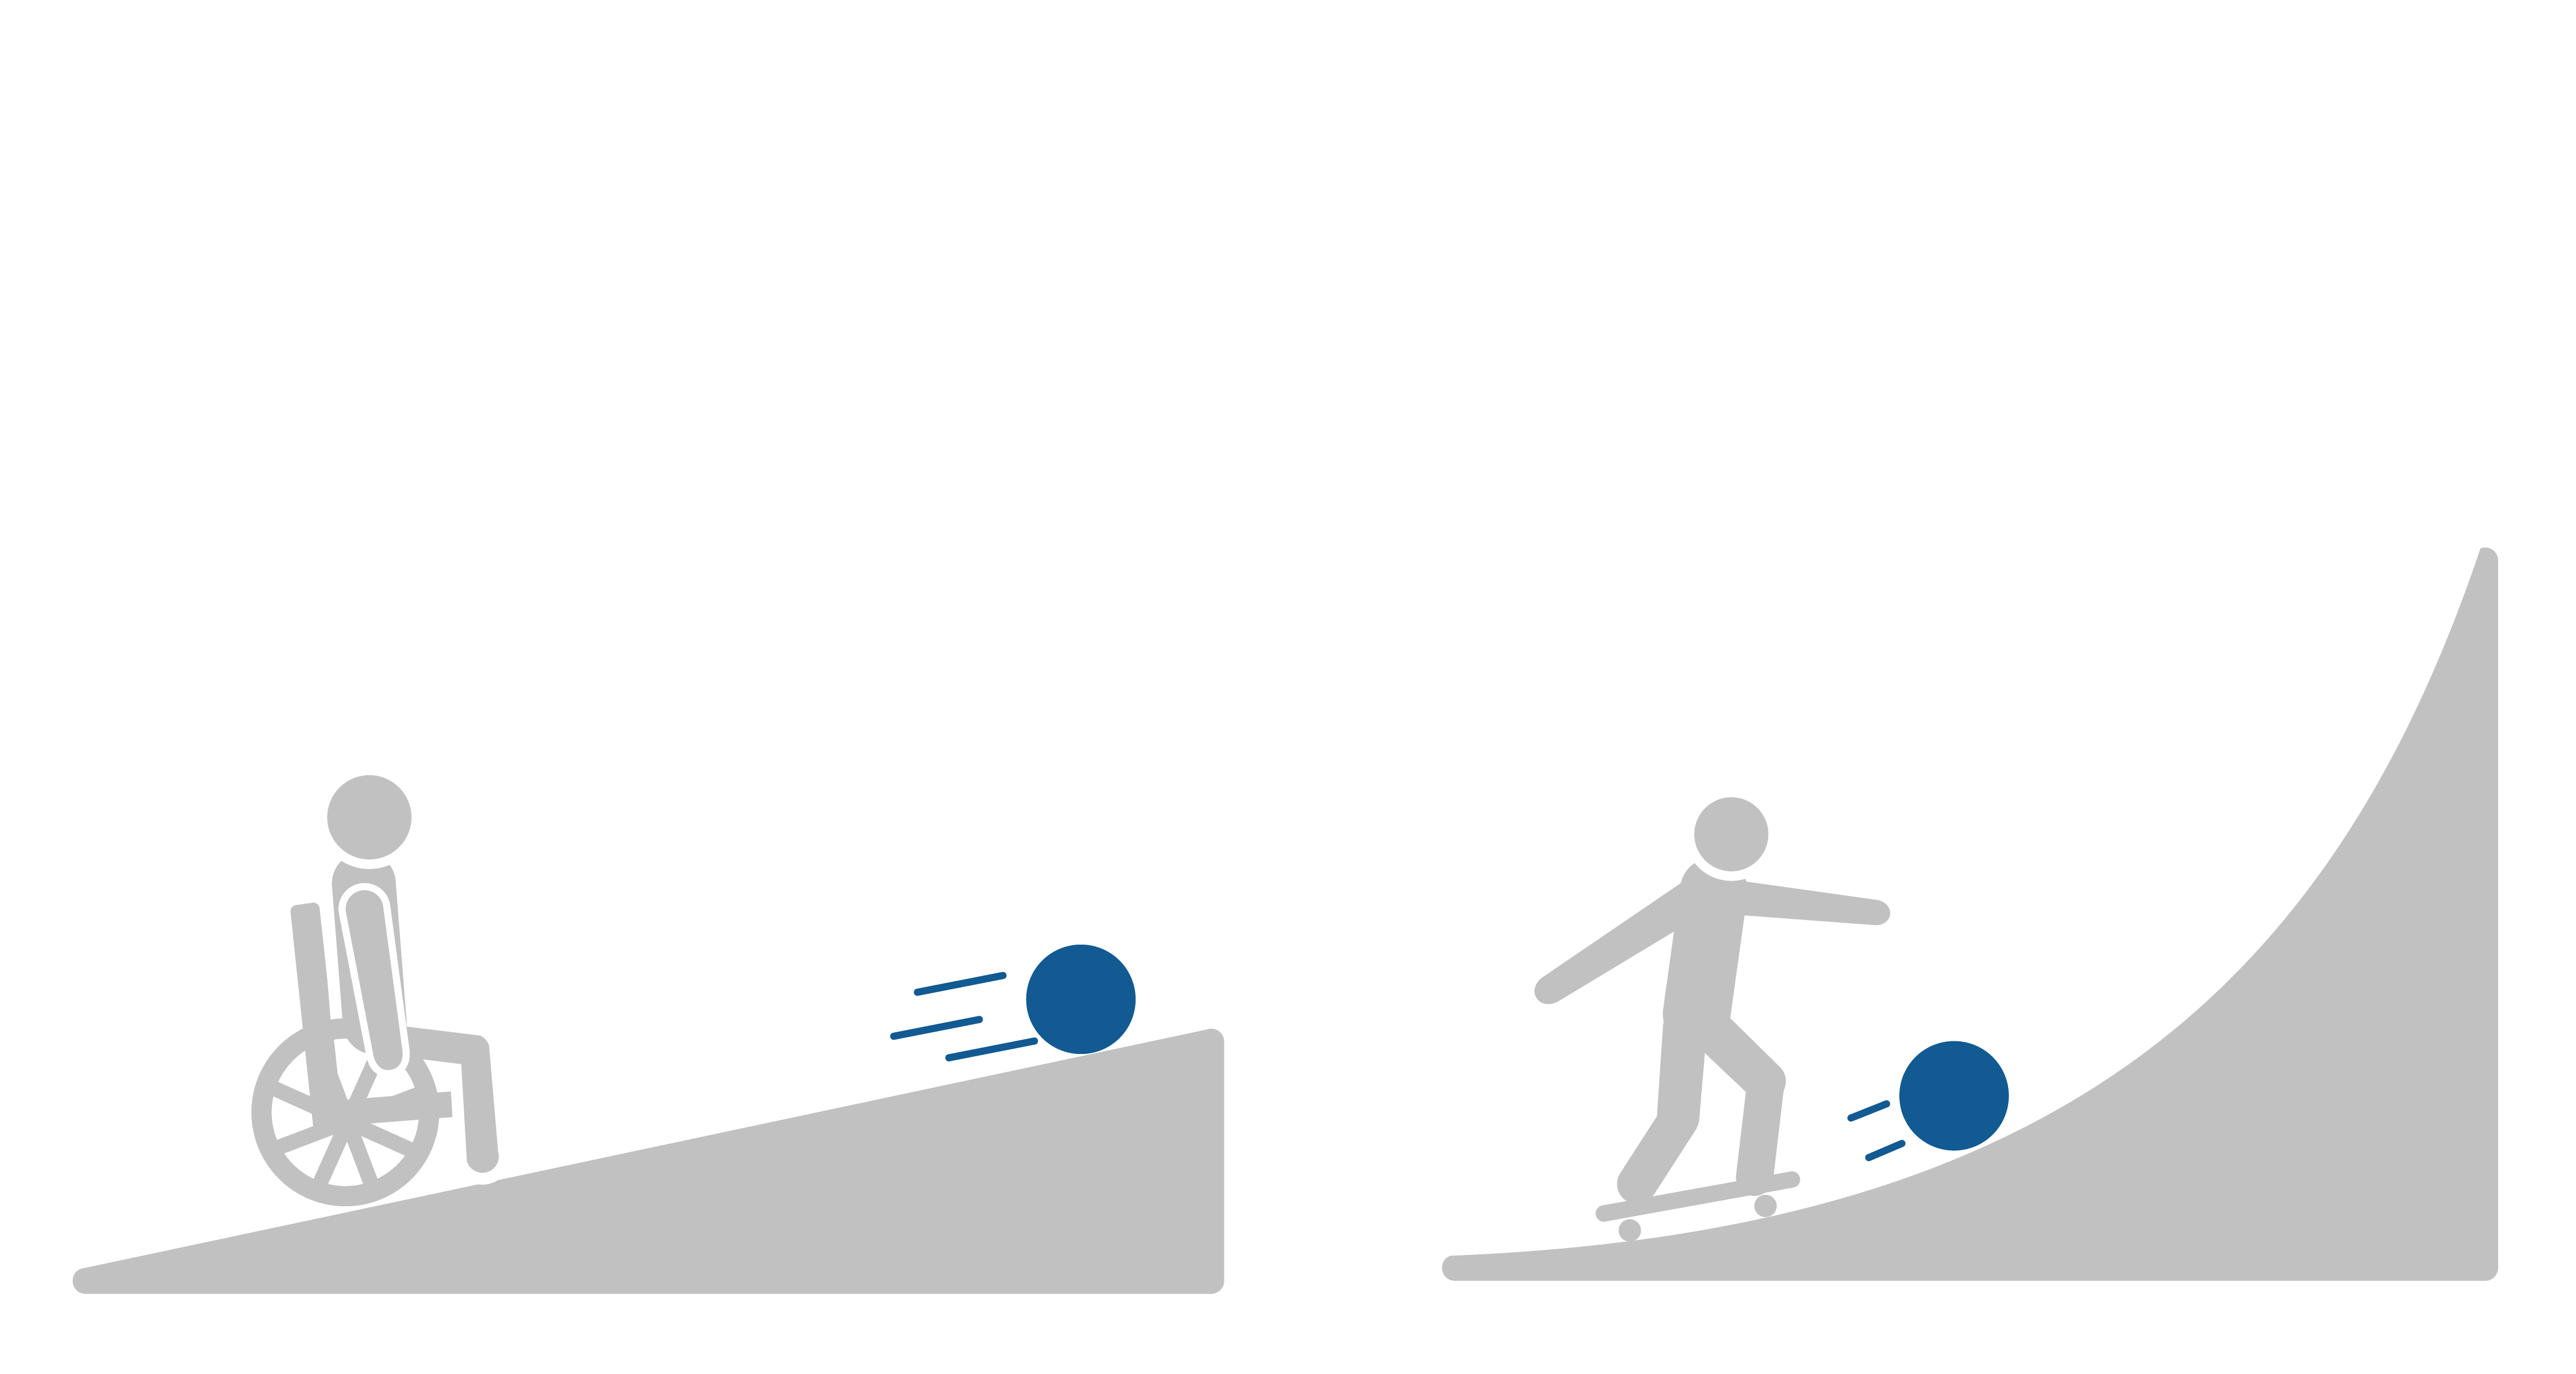
\includegraphics[width=\textwidth]{rampcomparison.png}

Assuming the incline has a constant steepness, the mechanical advantage is equal to the ratio of the length of the inclined plane to the height it rises.

If friction is neglected, the force required to push a weight up the inclined plane is given by:

\[
F_A = \frac{V}{L} F_G
\]

where \( F_A \) is the applied force, \( L \) is the length of the inclined plane, \( V \) is the vertical rise, and \( F_G \) is the gravitational force acting on the mass.

(We will discuss sine function later, but in case you're familiar with it, note that:

\[
\frac{V}{L} = \sin{\theta}
\]

where \( \theta \) is the angle between the inclined plane and the horizontal surface.)

\begin{Exercise}[title={Ramp}, label=ramp]
A barrel of oil weighs 136 kilograms. You can apply a force of up to 300 newtons. You need to get the barrel onto a platform that is 2 meters high. What is the shortest length of inclined plane you can use?
\end{Exercise}
\begin{Answer}[ref=ramp]
The weight of the barrel is \( 136 \times 9.8 = 1332.8 \) newtons.

Let \( L \) be the length of the inclined plane. The force needed to push the barrel up is related by:

\[
300 = \frac{2}{L} \times 1332.8
\]

Solving for \( L \), we find \( L = \frac{2 \times 1332.8}{300} \approx 8.885 \) meters.
\end{Answer}

\section{Gears}

Gears have teeth that mesh with each other. When you apply torque to one gear, it transfers torque to the other. The resulting torque is increased or decreased depending on the ratio of the number of teeth on the gears.

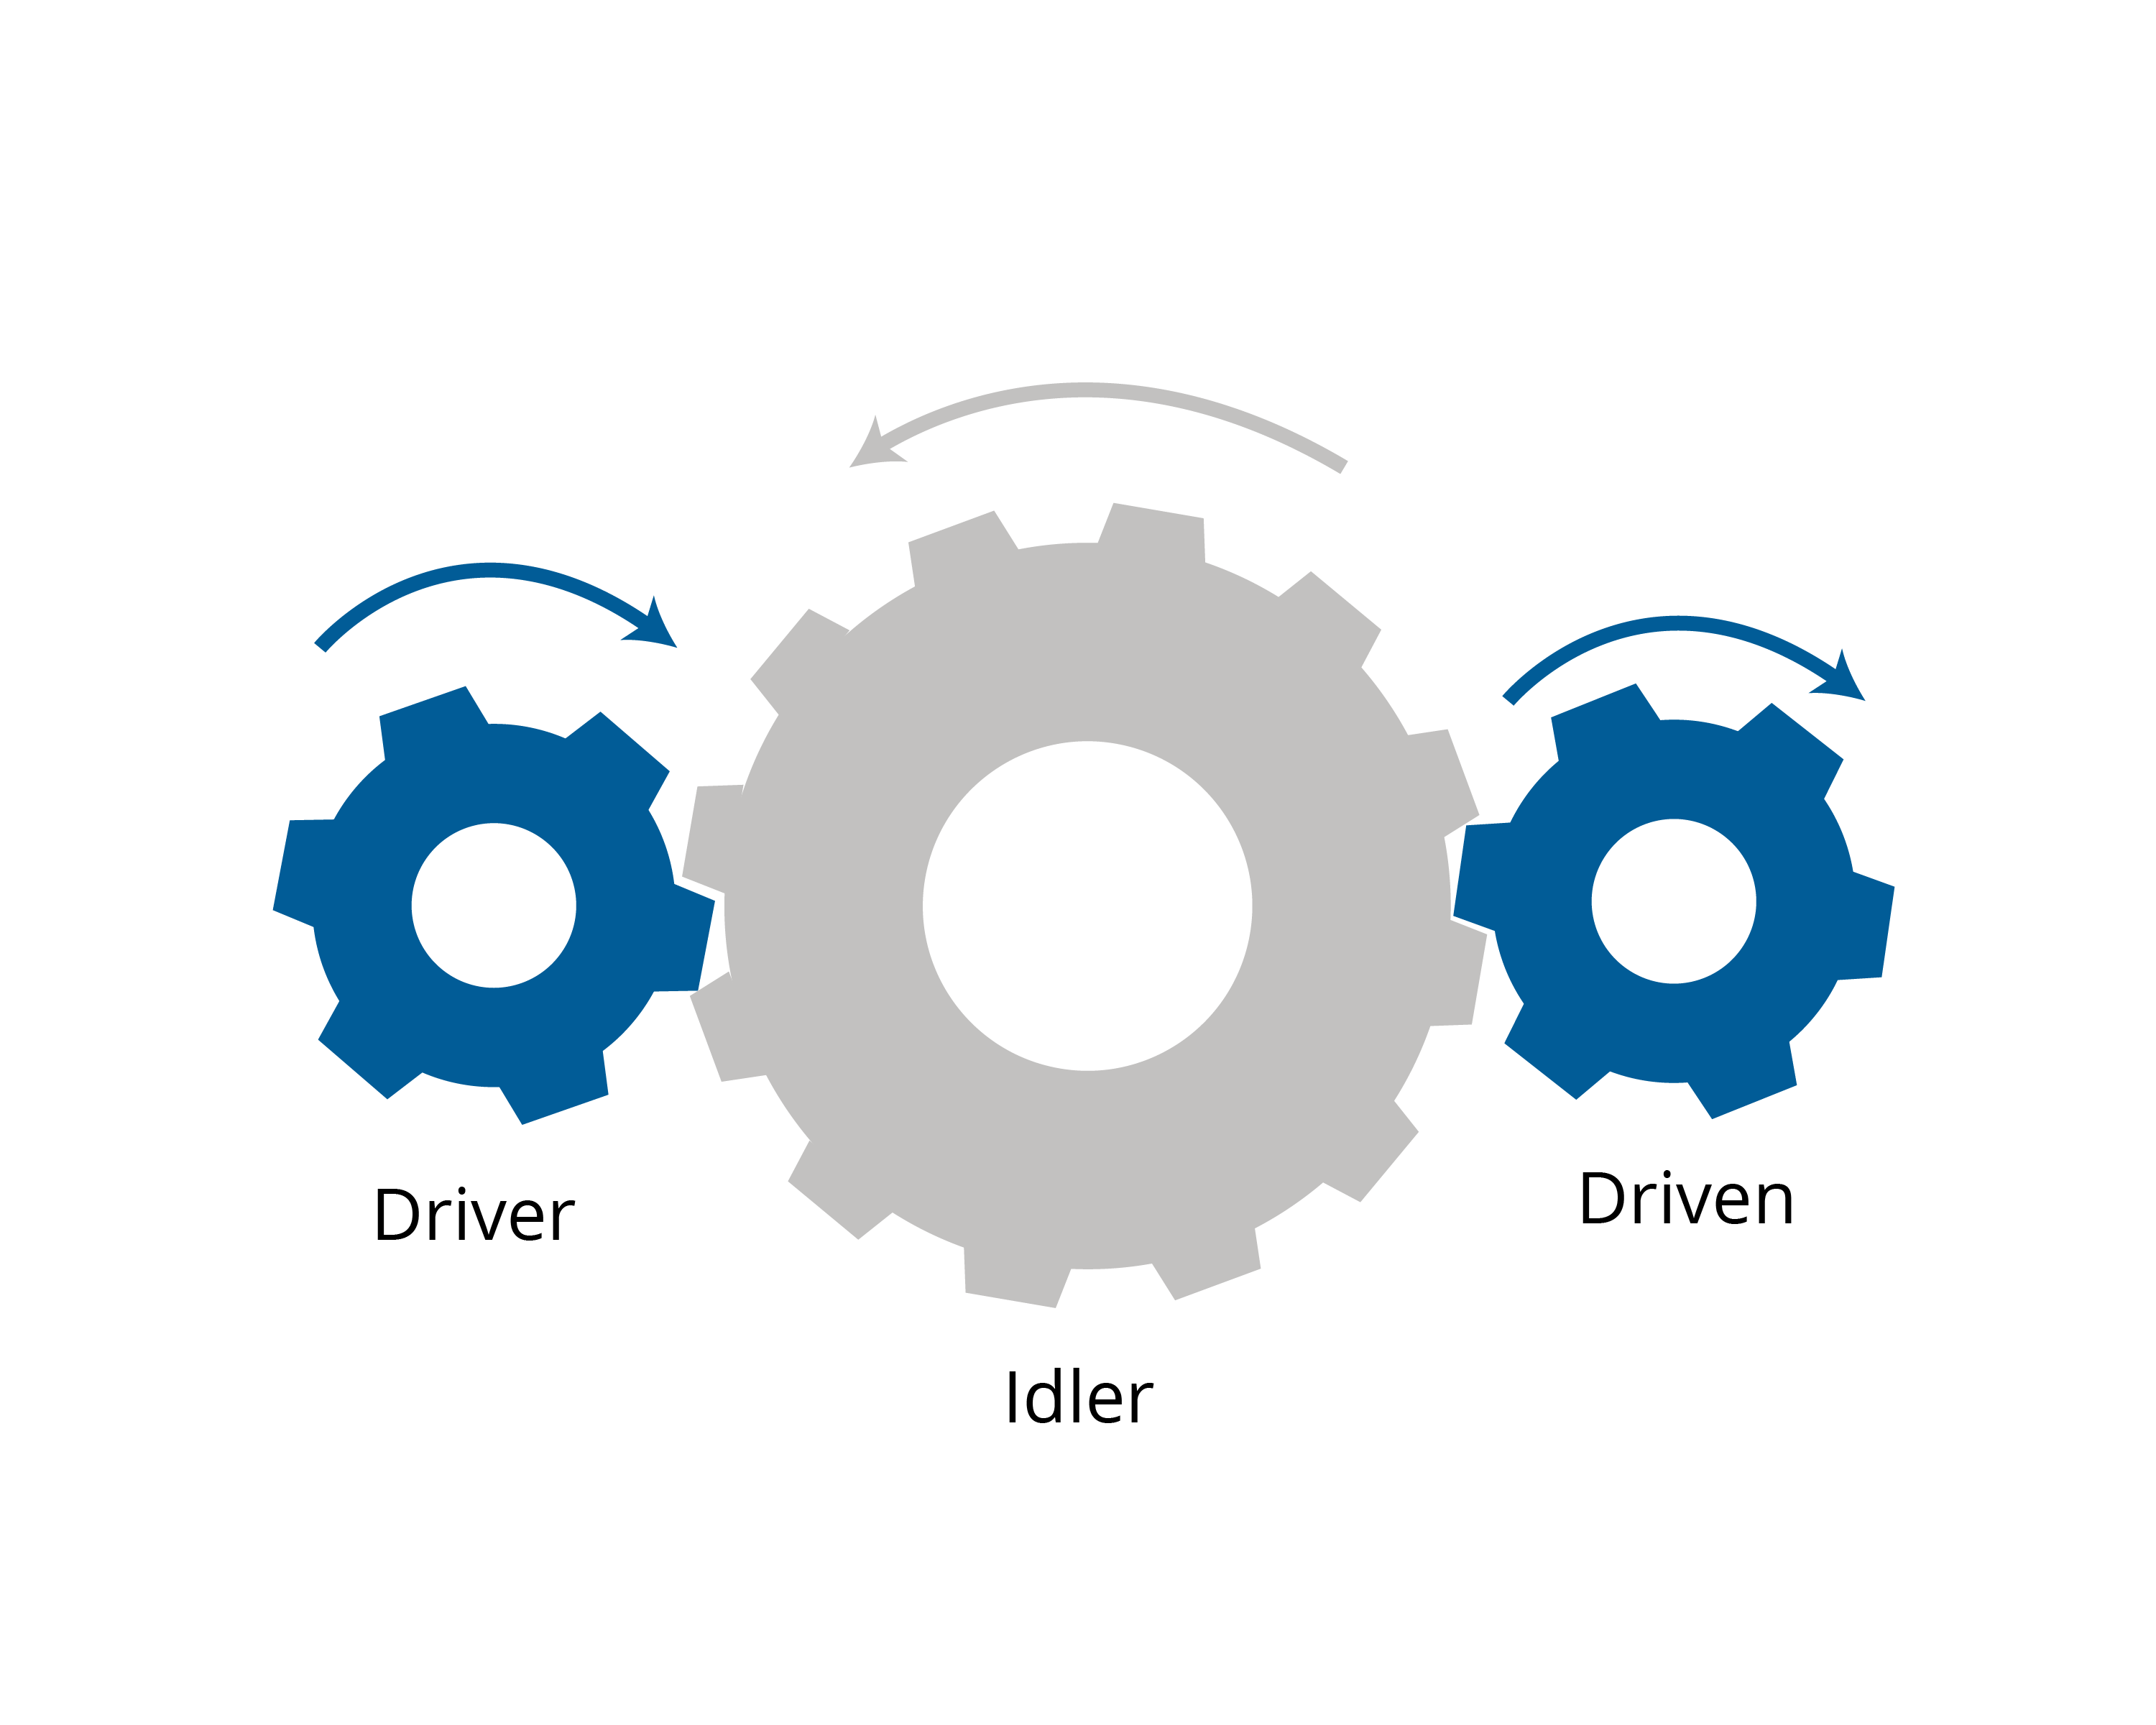
\includegraphics[width=0.7\textwidth]{gearsNew.png}

If \( N_A \) is the number of teeth on the gear you are turning with a torque of \( T_A \), and \( N_L \) is the number of teeth on the gear it is turning, the resulting torque is:

\[
T_L = \frac{N_A}{N_L} T_A
\]

\begin{Exercise}[title={Gears}, label=gear]
In a bicycle, the goal is not always to gain mechanical advantage, but to spin the pedals slower while applying more force.

You like to pedal your bike at 70 revolutions per minute. The chainring connected to your pedals has 53 teeth. The circumference of your tire is 2.2 meters. You want to ride at 583 meters per minute.

How many teeth should the rear sprocket have?
\end{Exercise}
\begin{Answer}[ref=gear]
The equation relating these quantities is:

\[
583 = 70 \times 2.2 \times \frac{53}{n}
\]

Solving for \( n \), we find \( n = 14 \) teeth.
\end{Answer}

\section{Hydraulics}

In a hydraulic system, such as a car's braking system, you exert force on a piston filled with fluid. The fluid transmits this pressure into another cylinder, where it pushes yet another piston that moves the load.

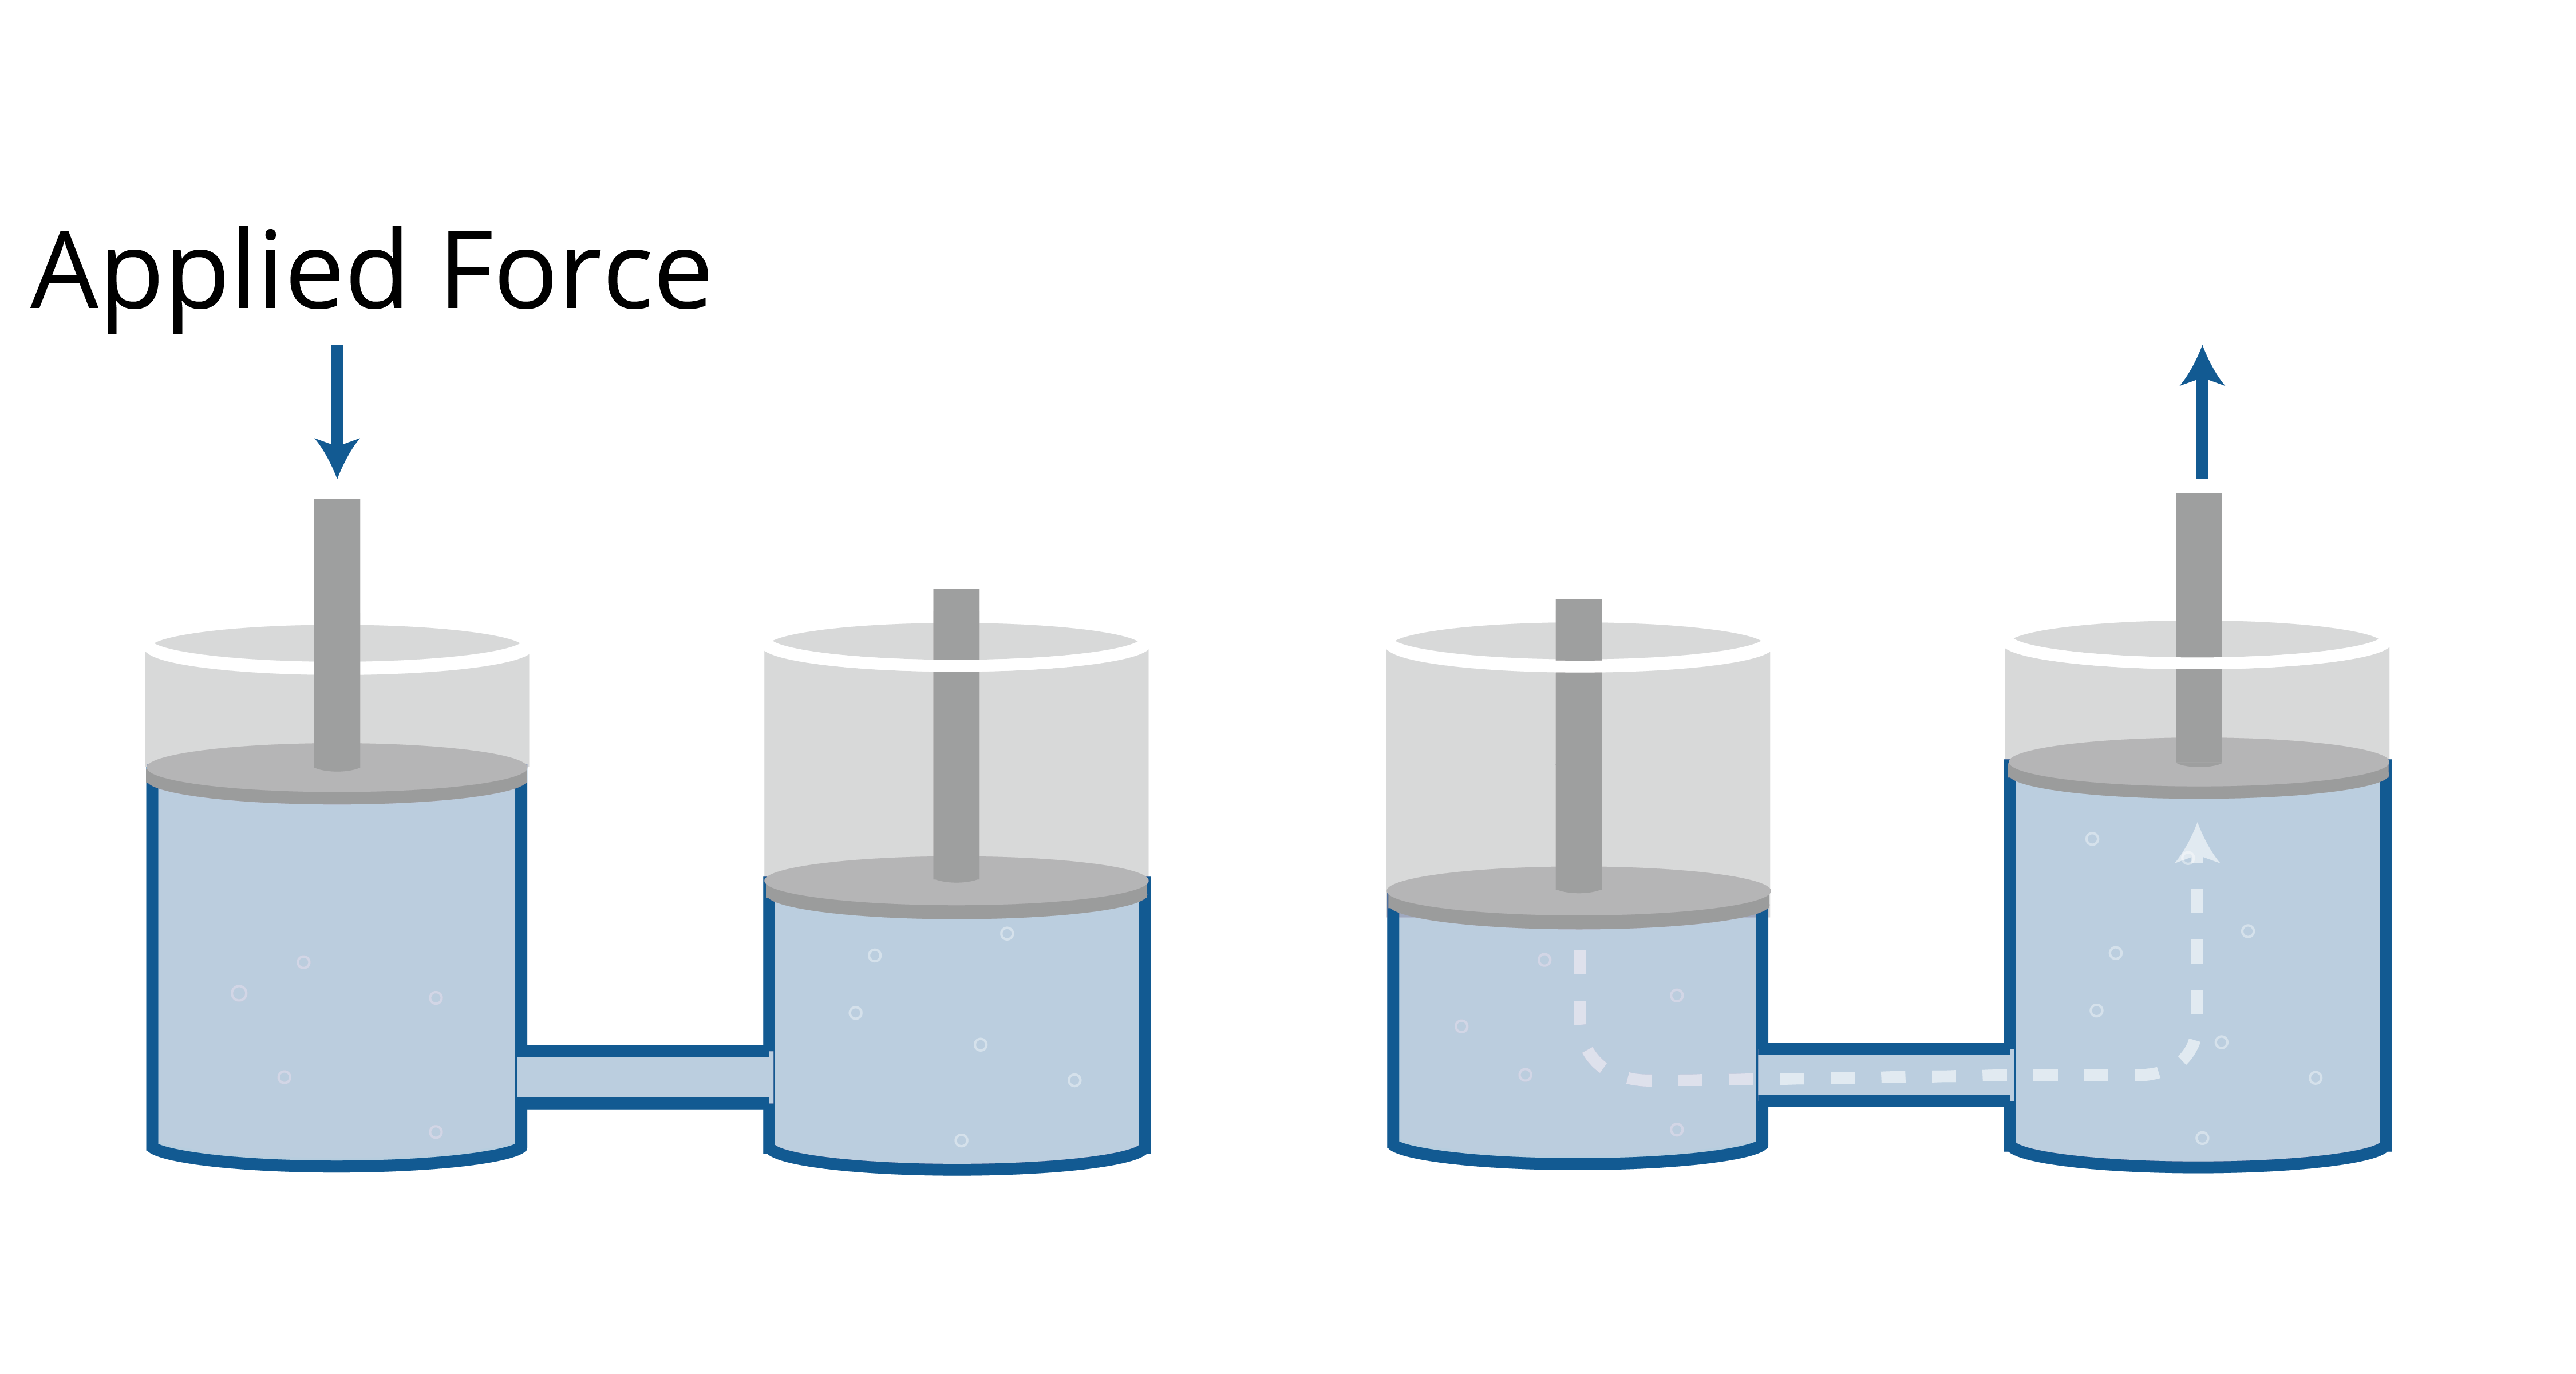
\includegraphics[width=\textwidth]{hydraulicsNew.png}

The pressure in the fluid is typically measured in pascals (Pa), which is equivalent to \(N / m^2\). We will use pascals for this calculation.

To calculate the pressure you create, divide the force applied by the area of the piston head. To determine the force on the other piston, multiply the pressure by the area of the second piston.

\begin{Exercise}[title={Hydraulics}, label=hydraulics]
Your car has disc brakes. When you apply 2,500,000 pascals of pressure to the brake fluid, the car stops quickly. As the car designer, you want this to require only 12 newtons of force from the driver's foot.

What should the radius of the master cylinder (the piston the driver pushes) be?
\end{Exercise}
\begin{Answer}[ref=hydraulics]
We are solving for the radius \( r \) of the piston. The area of the piston is \( \pi r^2 \), so the pressure is:

\[
\text{Pressure} = \frac{12}{\pi r^2}
\]

Setting the pressure equal to 2,500,000 pascals:

\[
2,500,000 = \frac{12}{\pi r^2}
\]

Solving for \( r \), we find:

\[
r = \sqrt{\frac{12}{\pi \times 2.5 \times 10^6}} \approx 0.00124 \text{ meters}.
\]
\end{Answer}

\graphicspath{{../../Chapters/buoyancy/en_US}}
\chapter{Buoyancy}

The word buoyancy probably brings to mind images of floating in water. Before we dive in, let's zoom out for a better understanding of everything buoyancy entails. You may be thinking: I want to be a computer programmer, why do I need to know about buoyancy? You might be surprised! This topic is much bigger than it seems at first glance. 

Buoyancy concerns the ways in which liquids and gasses interact with gravity. The concept of buoyancy is connected to fundamental concepts about how the universe works. The \newterm{buoyant force}, as it is known in engineering, is an important concept that has wide ranging applications. A big part of engineering is moving stuff around, and understanding buoyancy helps us solve problems where we need to move things in and through fluids. Even if you don't have plans to build a robotic submarine, these are incredibly useful ideas to be familiar with. We will start exploring the topic with familiar scenarios around boats and water.

When you put a boat into water, it will sink into the water until
the mass of the water it displaces is equal to the mass of the
boat. We think of this in terms of forces. Gravity pulls the mass of
the boat down; the \newterm{buoyant force} pushes the boat up. A boat
dropped into the water will bob up and down at first before reaching an
\newterm{equilibrium} where the two forces are equal.
% FIXME: Define displacement, and velocity. It is not defined in workbook one or this chapter (I think that would help) - Arjan
% ADD: Explain Action Reaction Pairs in previous chapter
% ADD: Archimedes principle

The buoyant force pushes things up, fighting against the force of
gravity. The force is equal to the weight of the fluid being
replaced. For example, a cubic meter of freshwater has a mass of
about 1000kg. If you submerge anything with a volume of one meter in
freshwater on earth, the buoyant force will be about 9800 newtons ($\text{mass} \times \ \text{gravity})$.

For some things, like a block of styrofoam, this buoyant force will be
sufficient to carry it to the surface. Once it reaches the surface, it
will continue to rise (displacing less water) until the mass of the
water it displaces is equal to its mass. And then we say ``It floats!''

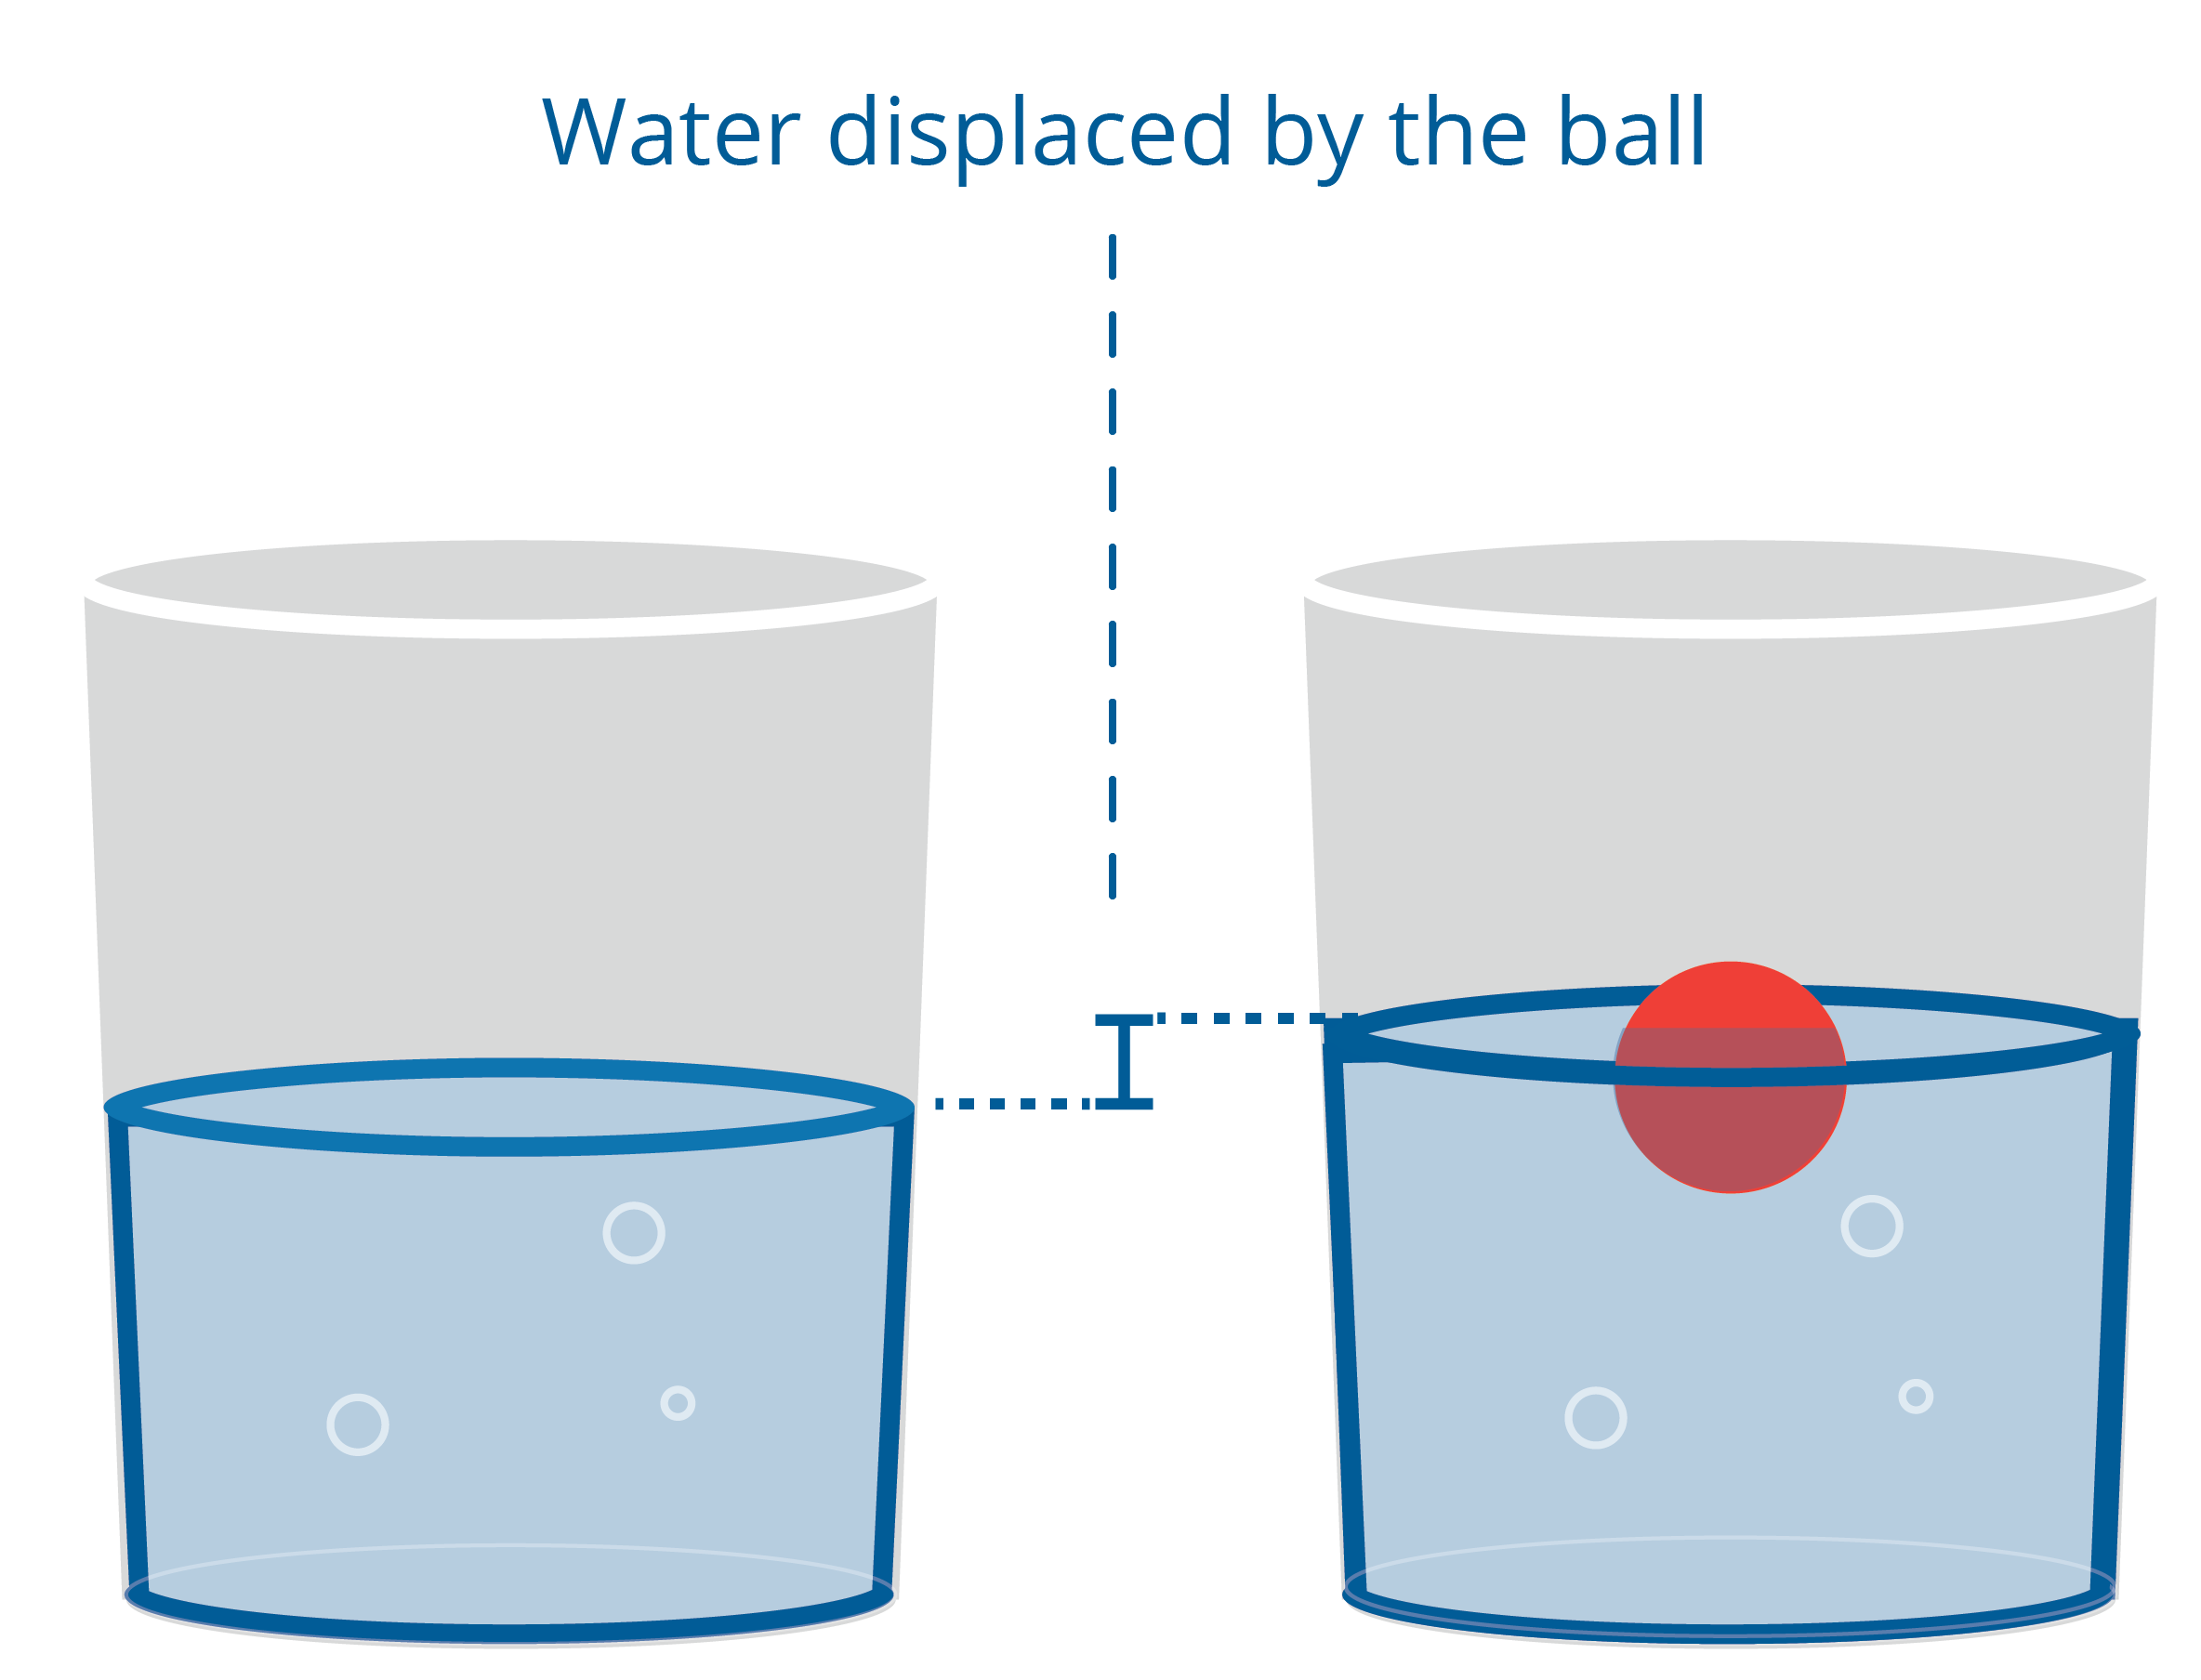
\includegraphics[width=.6\textwidth]{waterDisplacement.png}

For some things, like a block of lead, the buoyant force is not
 sufficient to lift it to the surface, and then we say ``It sinks!''

This is why a helium balloon floats through the air. The air
that it displaces weighs more than the balloon and the helium itself. (It is easy to forget that air has a mass, but it does.)

\begin{Exercise}[title={Buoyancy}, label=buoyancy]
  You have an aluminum box that has a heavy base, so it will always
  float upright. The box and its contents weigh 10 kg. Its base is 0.3 m x 0.4 m. It is 1m tall.

  When you drop it into freshwater ($1000 kg/m^3$), how far will it sink
  before it reaches equilibrium?\index{equilibrium}

\end{Exercise}
\begin{Answer}[ref=buoyancy]
  Equilibrium will be achieved when the box has displaced 10 kg of water. In other words, when it has displaced $0.01$ cubic meters.

  The area of the base of the box is 0.12 square meters. So if the
  box sinks $x$ meters into the water it will displace $0.12 x$ cubic
  meters.

  Thus at equilibrium $x = \frac{0.01}{0.12} \approx 0.083$ m. So
  the box will sink 8.3 cm into the water before reaching equilibrium.
\end{Answer}

\section{The Mechanism of Buoyancy: Pressure}

As you dive down in the ocean, you will experience greater and
greater pressure from the water. And if you take a balloon with you, you
will gradually see it get smaller as the water pressure compresses the
air in the balloon.

Let's say you are 3 meters below the surface of the water. What is the
pressure in Pascals (newtons per square meter)? You can think of the
water as a column of water crushing down upon you. The pressure over
a square meter is the weight of 3 cubic meters of water pressing down.

$$p = (3)(1000)(9.8) = 29,400 \text{ Pa }$$

This is called \newterm{hydrostatic pressure}. The general rule for
hydrostatic pressure in Pascals $p$ is

$p = d g h$

where $d$ is the density of the fluid
in kg per cubic meter, $g$ is the acceleration due to gravity in
$m/s^2$, and $h$ is the height of the column of fluid above you.

So where does buoyant force come from? Basically, the pressure pushing up on the
deepest part of the object is higher than the pressure pushing down on
the shallowest part of the object. That is where bouyancy comes from.

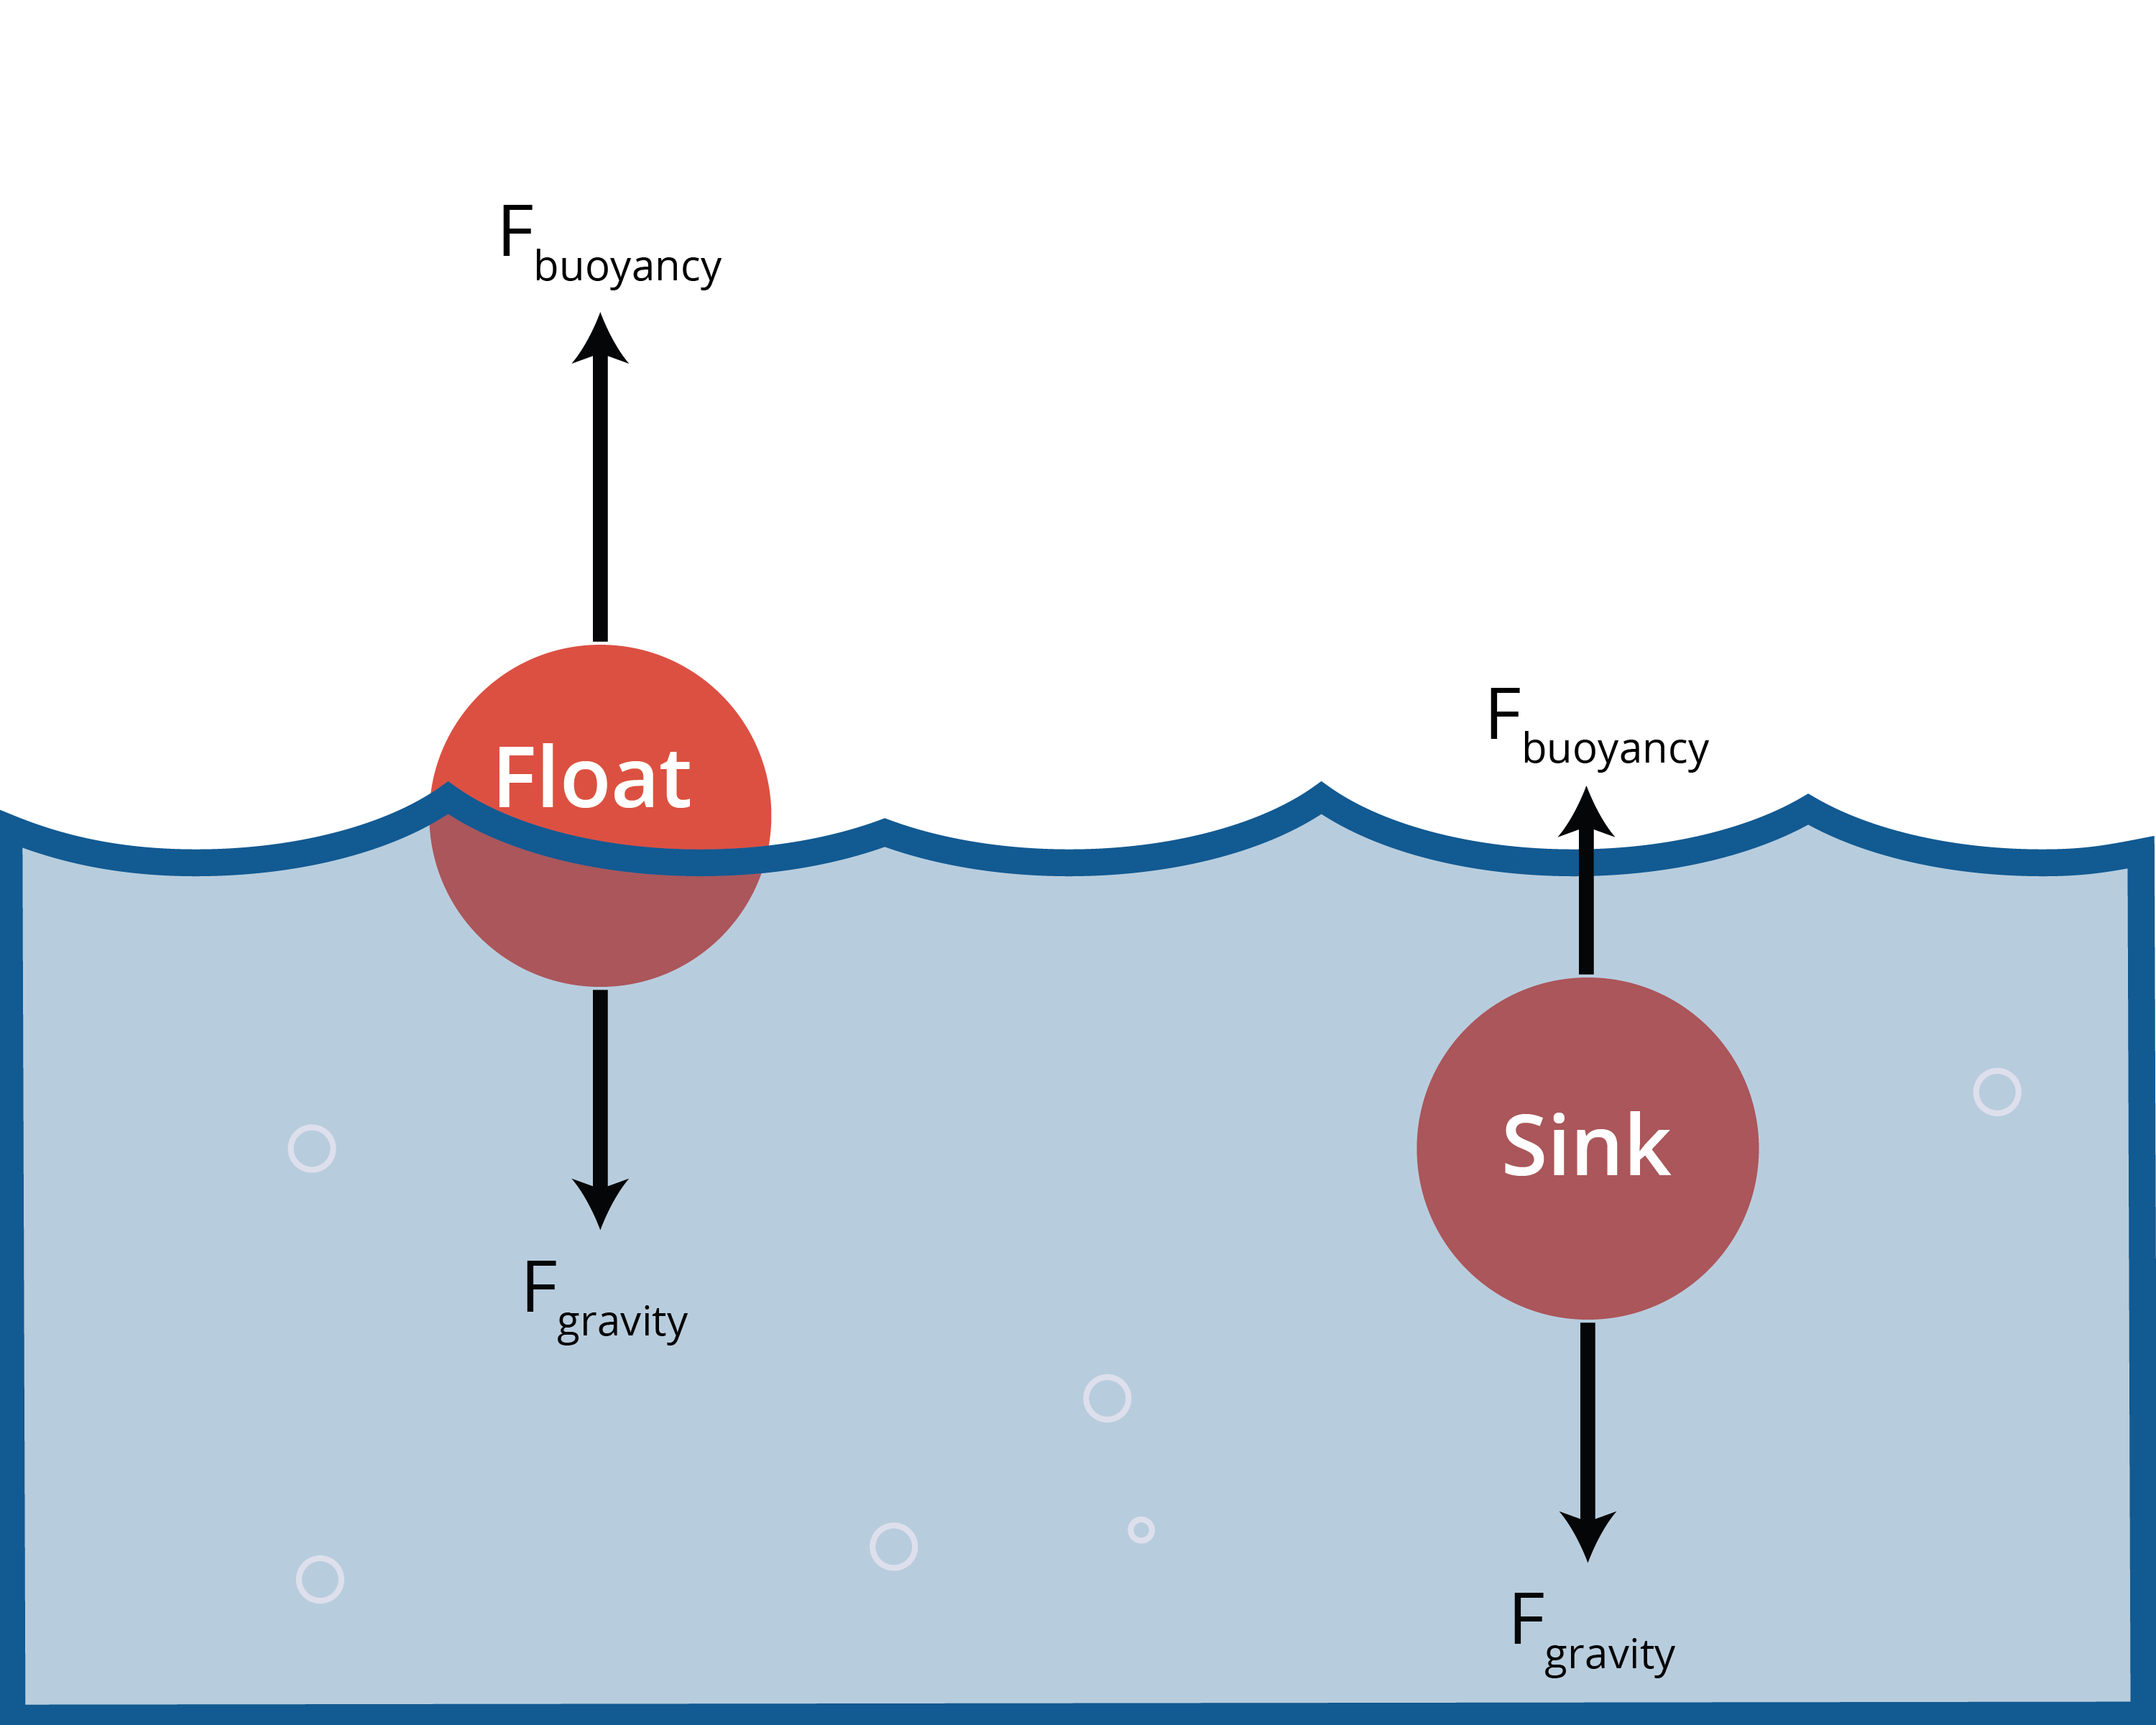
\includegraphics[width=.6\textwidth]{buoyancy.png}

\begin{Exercise}[title={Hydrostatic Pressure}, label=mars_pressure]

  You dive into a tank of olive oil on Mars. How much more
  hydrostatic pressure does your body experience at 5 meters deep than
  it did at the surface?

  The density of olive oil is about 900 kg per square meter. The
  acceleration due to gravity on Mars is 3.721 $m/s^2$.

\end{Exercise}
\begin{Answer}[ref=mars_pressure]
$$p = d g h = (900)(3.721)(5) = 16,744.5 \text{ Pa}$$
\end{Answer}

\section{The Mechanism of Buoyancy: Density}
Keep in mind that although the pressure is increasing as you go deeper, the
buoyant force will \emph{not increase}, because the buoyant force is always equal
to the weight of the fluid that is displaced, regardless whether that is 1
meter or 100 meters underwater.

Due to the added minerals, saltwater is denser than freshwater. This causes objects to float
better in the sea than they do in a river. Lipids, like fats and
oils, are less dense than water, allowing them to float on top of a glass of water.
When you're facing a grease fire, you're told not to put water on it. That's because
the water sinks below the grease, then boils, throwing burning grease everywhere.

\graphicspath{{../../Chapters/heat/en_US}}
\chapter{Heat}

All mass in the universe has heat, whether you're looking at a block of dry ice (frozen $CO_2$, $-78.5^\circ$ C)
or the surface of the sun ($5,600^\circ$ C). As long as the mass is above absolute zero --- the coldest possible
temperature in the universe --- there is some amount of heat in it.

\section{How Heat Works}

As you heat up an object, you are imparting energy into it. Where does this energy go? The atoms take this energy
and they begin to move, vibrating and bumping into each other, causing the heat to spread throughout. Everytime the
atoms collide and bounce off of each other, they emit a tiny amount of energy as light. In most cases, that light is
in the infrared spectrum, but in extreme cases can be visible, such as with molten lava or hot metal.

As objects interact, they either put heat into colder objects or take heat from warmer objects. That's what allows you to heat up
anything in the first place. The hot air from a stove or bunsen burner interacts with the pan or test tube you're heating,
passing the air's heat on. How could you model this?

\section{Specific Heat Capacity}

If you are heating something, the amount of energy you need to
transfer to it depends on three things: the mass of the thing you are
heating, the amount of temperature change you want, and the
\textit{specific heat capacity} of that substance.\index{specific heat capacity}

\begin{mdframed}[style=important, frametitle={Energy in Heat Transfer}]

  The energy moved in a heat transfer is given by

  $$E = m c \Delta_T$$

  where $m$ is the mass, $\Delta_T$ is the change in temperature, and
  $c$ is the specific heat capacity of the substance.
% ADD: q=mcat

  (Note that this
  assumes there isn't a phase change. For example, this formula works nicely on
  warming liquid water, but it gets more complicated if you warm the
  water past its boiling point.)

\end{mdframed}

Can we guess the specific heat capacity of a substance? It is very,
very difficult to guess the specific heat of a substance, so we determine
it by experimentation.

For example, it takes 0.9 joules to raise
the temperature of solid aluminum one degree Celsius. So we say ``The
specific heat capacity of aluminum is 0.9 J/g $^\circ$C.''

The specific heat capacity of liquid water is about 4.2 J/g $^\circ$C.

Let's say you put a 1 kg aluminum pan that is $80^\circ$ C into
3 liters of water that is $20^\circ$ C. Energy, in the form of heat,
will be transferred from the pan to the water until they are at the same
temperature. (We call this ``thermal equilibrium.'')\index{thermal equilibrium}

What will the temperature of the water be?

To answer this question, the amount of energy given off by the
pan must equal the amount of energy absorbed by the water. They also
need to be the same temperature at the end. Let $T$ be the final
temperature of both.

3 liters of water weighs 3,000 grams, so the
change in energy in the water will be:

$$E_W = m c \Delta_T = (3000)(4.2)(T - 20) = 12600T - 252000 \text{ joules}$$

The pan weighs 1000 grams, so the change in energy in the pan will be::

$$E_P = m c \Delta_T = (1000)(0.9)(T - 80) = 900T - 72000 \text{ joules}$$

The total energy stays the same, so $E_W + E_P = 0$. This means you need to solve

$$(12600T - 252000) + (900T - 72000) = 0$$

And find that the temperature at equilibrium will be

$$T = 24^\circ \text{C}$$

\begin{Exercise}[title={Thermal Equilibrium}, label=thermal_equilibrium]

Just as you put the aluminium pan in the water as described above,
someone also puts a 1.2 kg block of copper cooled to 10 $^\circ$ C.
The specific heat of solid copper is about 0.4 J/g $^\circ$C.

What is the new temperature at equilibrium?

\end{Exercise}
\begin{Answer}[ref=thermal_equilibrium]

  $$E_C = (1200)(0.4)(T - 10) = 480T - 4800$$

Total energy stays constant:

$$0 = (12600T - 252000) + (900T - 72000) + (480T - 4800)$$

Solving for $T$ gets you $T = 23.52^\circ$ C.

\end{Answer}

\section{Getting to Equilibrium}

When two objects with different temperatures are touching, the speed
at which they exchange heat is proportional to the differences in
their temperatures. As their temperatures get closer together,
the heat exchange slows down.
% ADD: explain which object, water or metal has a greater tempature change

In our example, the pan and the water will get close to equilibrium
quickly, but they may never actually reach equilibrium.

\begin{tikzpicture}
    \begin{axis}[
        xmin=0,xmax=4.25,
        ymin=15,ymax=85,
        axis x line=middle,
        axis y line=middle,
        axis line style=<->,
        xlabel={minutes},
        ylabel={degrees celsius},
        ]
        \addplot[no marks,sdkblue] expression[domain=0:4,samples=100]{24 + 56 * pow(2,-1.5 * x)} node[above, xshift=-1cm, yshift=0.1cm]{Pan};
        \addplot[no marks,sdkblue] expression[domain=0:4,samples=100]{24 - 4 * pow(2,-0.8 * x)} node[below, xshift=-2.5cm]{Water};
        \addplot[no marks,dashed,gray] coordinates {(0,24)(6,24)} node[above, xshift=-8cm]{equilibrium};
    \end{axis}
\end{tikzpicture}

\begin{Exercise}[title={Cooling Your Coffee}, label=cool_coffee]

  You have been given a ridiculously hot cup of coffee and a small pitcher of chilled milk.

  You need to start chugging your coffee in three minutes, and you want it as cool as possible at that time. When should you add the milk to the coffee?

\end{Exercise}
\begin{Answer}[ref=cool_coffee]

  During the 3 minutes, you want the coffee to give off as much of its
  heat as possible, so you want to maximize the difference between the
  temperature of the coffee and the temperature of the room around
  it.

  You wait until the last moment to put the milk in.

\end{Answer}

\section{Specific Heat Capacity Details}

For any given substance, the specific heat capacity often changes a
great deal when the substance changes state. For example, ice is 2.1 J/g
$^\circ$C, whereas liquid water is 4.2 J/g$^\circ$C.

Even within a given state, the specific heat capacity varies a bit
based on the temperature and pressure. If you are trying to do these
sorts of calculations with great accuracy, you will want to find the
specific heat capacity that matches your situation. For example, I
might look for the specific heat capacity for water at $22^\circ$C at
1 atmosphere of pressure (atm).

%%%%%%%%%%%%%%%%%%%%%%%%%%%%%%%%%
%% Bookfooter.tex by Aaron Hillegass
%% Nov 8, 2020

\appendix

\chapter{Answers to Exercises}
\shipoutAnswer

\bibliography{references}

\printindex

\end{document}